\documentclass[12pt,reqno]{nuthesis}	% The nuthesis class is based on amsbook.cls.

%\usepackage{mathptmx}
%\usepackage{times}
%\renewcommand{\familydefault}{\sfdefault}

% paragraph spacing
\setlength{\parindent}{0.5in} % indentation of paragraphs
\setlength{\parskip}{5pt} % gap between paragraphs

% figures
\usepackage[margin=1in,letterpaper,includehead]{geometry}
\usepackage{graphicx}
\graphicspath{ {./figures/} } % define graphics location

% figure setting
%\setlength{\textfloatsep}{0.25in} % space between last top float or first bottom float and the text.
%\setlength{\floatsep}{0.5in} % space left between floats.
%\setlength{\intextsep}{0.25in} % space left on top and bottom of an in-text float.  
\setlength{\textfloatsep}{15pt plus 3pt minus 2pt} % space between last top float or first bottom float and the text.
\setlength{\intextsep}{15pt plus 3pt minus 2pt} % space left on top and bottom of an in-text float.  
\setlength{\floatsep}{15pt plus 3pt minus 2pt} % space left between floats.
\setlength{\abovecaptionskip}{10pt plus 3pt minus 3pt} % space above caption
\setlength{\belowcaptionskip}{3pt plus 2pt minus 1pt} % space below caption

% captions
\usepackage{ccaption}
\usepackage[margin=0in,skip=5pt,font={footnotesize,bf},labelfont=bf]{caption}
\captionsetup[figure]{margin=20pt}
%\usepackage{subcaption}

% tables
\usepackage{array}
\usepackage{multirow}
\usepackage{booktabs}

% formulas and symbols
\usepackage{mathtools}
\usepackage{amsmath,amssymb}
\DeclareMathOperator*{\argmax}{\arg\!\max} % argmax formatter
\DeclareMathOperator*{\argmin}{\arg\!\min} % argmin formatter
\usepackage{siunitx} % scientific notation
\usepackage{extarrows} % arrows
\usepackage[euler]{textgreek} % greek characters
\usepackage{textcomp} % degrees C
\mathchardef\hyphy="2D % hyphen for mathmode

% links
\usepackage{hyperref}
\usepackage{enumitem}

% references formatting
\usepackage[numbers,sort&compress]{natbib}

% additional tools
%\usepackage{comment}
%\sloppy

\usepackage[activate={true,nocompatibility},final,tracking=true,kerning=true,spacing=true,factor=1050,stretch=10,shrink=10]{microtype}
\microtypecontext{spacing=nonfrench}
% activate={true,nocompatibility} - activate protrusion and expansion
% final - enable microtype; use "draft" to disable
% tracking=true, kerning=true, spacing=true - activate these techniques
% factor=1100 - add 10% to the protrusion amount (default is 1000)
% stretch=10, shrink=10 - reduce stretchability/shrinkability (default is 20/20)

%%%%%%%%%%%%%%%%%%%%%%%%%%%%%%%%%%%%%
% USER-DEFINED MACROS AND VARIABLES %
%%%%%%%%%%%%%%%%%%%%%%%%%%%%%%%%%%%%%

% vertically centered and horizontally centered column
\newcolumntype{C}[1]{>{\centering\arraybackslash}m{#1}}

% vertically centered and horizontally right-aligned column
\newcolumntype{R}[1]{>{\raggedleft\arraybackslash}m{#1}}

% vertically centered and horizontally left-aligned column
\newcolumntype{L}[1]{>{\raggedright\arraybackslash}m{#1}}

% Always capitalize "Chapter" when using \autoref
%\renewcommand{\chapterautorefname}{Chapter}

%%%%%%%%%%%%%%
% TITLE PAGE %
%%%%%%%%%%%%%%

\author{Sebastian Michal Bernasek}

\title{Quantitative analysis of cell fate decisions}

\degree{DOCTOR OF PHILOSOPHY}

\field{Chemical and Biological Engineering}           

\graduationmonth{June}         
                             
\graduationyear{2019}          

%%%%%%%%%%%%%%%%%%%%%%%%
% DISSERTATION CONTENT %
%%%%%%%%%%%%%%%%%%%%%%%%
		
\begin{document}
\frontmatter		
\maketitle		
\copyrightpage	

% abstract
\abstract       




Cell fate decision mechanisms are notoriously difficult to quantitatively characterize. Chapter \ref{ch:clones} introduces a computational framework for automated quantitative analysis of genetic mosaics; a class of experiments designed to probe gene expression \textit{in vivo}. The framework combines computer vision and statistics to measure protein levels in individual cells and predict their respective genotypes. It thereby facilitates systematic quantitative comparison of expression levels between cells subject to control and perturbation conditions. The accompanying software eliminates each of the labor-intensive steps of a quantitative workflow, and will hopefully lower the barrier to adoption of quantitative analysis strategies. 

Chapter \ref{ch:ratio} explores a novel cell fate decision mechanism underlying photoreceptor specification in the developing fruit fly eye. Computer vision and statistical modeling techniques are used to extract quantitative measurements of transcription factor dynamics from a wealth of confocal microscopy data. These data show that differentiation is driven by dynamic changes in the ratio between two transcription factors, and is agnostic to changes in their absolute concentrations as long as the ratio remains constant. A general model based on the statistical physics of transcription factor DNA binding shows that this phenomenon is a natural consequence of competition between the two transcription factors for common binding sites. The findings add a new dimension to our understanding of how transcription factors coordinate cell fate decisions, and showcase the importance of both quantitative and dynamic measurements for characterizing developmental systems. 

Chapter \ref{ch:metabolism} proposes a novel theory to explain why the regulatory networks that coordinate cell fate decisions often contain several repressors tasked with attenuating expression of a single target gene. The theory posits that auxiliary negative regulators enable development to proceed more quickly by mitigating erroneous cell fate decisions when cells are rapidly metabolizing. It is supported by a robust collection of qualitative experiments showing that a broad variety of repressor loss-of-function phenotypes are reversed when biosynthesis rates are artificially slowed. A quantitative modeling framework is used survey a hypothesized mechanistic origin of this effect. Namely, that auxiliary repressors help avert erroneous decisions by expanding cells capacity to buffer excess protein expression. Quantitative measurements of transcription factor activity serve to validate the predictions made by the modeling framework. As shorter developmental times confer a selective advantage upon organisms, these findings may represent a novel evolutionary driving force for increased robustness of cell fate decisions.

Beyond their insights into the mechanics of cell fate decisions, these efforts have spawned several computational tools that may prove valuable to the broader community (see \ref{appendix:software}). All such resources have been made freely available, and their continued development should help contribute toward the sustained prevalence of quantitative analysis of cell fate decisions.


% acknowledgements
\acknowledgements
I would like to thank the mentors, friends, family, and coffee growers whose support made this work possible.

% table of contents
\clearpage\phantomsection
\tableofcontents	

% list of figures
\clearpage\phantomsection
\listoffigures

% list of tables
\clearpage\phantomsection 
\listoftables	

% primary text
\mainmatter     
\chapter{Introduction}

The natural world presents a stunning variety of multicellular organisms. We tend to distinguish them by the physiological traits that define their stereotyped identities. For instance, we recognize penguins by their unusual stature, black and white fur, long beak, and impressive ability to wobble around on ice. These features are a culmination of many complex cellular processes collectively known as \emph{development}.

Development begins with a single cell, with subsequent growth and division events driving progression toward adulthood. Cells acquire increasingly specific roles and functions as growth proceeds, ultimately giving rise to stereotyped adult morphologies. This process, known as lineage restriction, demands that each cell decides to adopt the correct fate at the appropriate time and place.

Cell fate decisions are remarkably robust, yielding consistent phenotypes amidst the vast array of conditions encountered in natural environments. They are so reliable that we often take them for granted. For instance, it is difficult to imagine a scenario in which we might mistake another human for a penguin. However, they can and do exhibit minor variation that can have dire consequences for human health. Researchers therefore continue to study these complex processes in the hope that they might one day be able to control their behavior; either to exploit them in novel biotechnologies, or rectify the diseases that arise when they fail. Research efforts are predominantly motivated by two fundamental questions. First, how do cells make decisions? Second, how do they make them reliably? 

This dissertation addresses subtle aspects of both questions by combining chemical engineering, computer vision, and statistics to extract meaningful insight from experimental data. Chapter \ref{ch:clones} introduces a novel computational framework for automating the quantitative analysis of an existing class of experiments designed to probe cell fate decisions \textit{in vivo}. Chapter \ref{ch:ratio} elucidates a novel mechanism governing cell fate decisions in the developing fruit fly eye. Chapter \ref{ch:metabolism} explores a new evolutionary driving force for increased reliability of cell fate decisions. The remaining sections of this chapter serve to prime the reader with the context needed to situate the presented findings within the broader literature. 

\section{Molecular origins of cell fate decisions}

Early experiments in a variety of model organisms demonstrated that cell fate decisions are encoded in the genome. Genetics were therefore believed to provide a predefined road map for the tortuous journey from embryo to adulthood, inspiring researchers throughout the twentieth century to probe the roles of individual genes in coordinating adult phenotypes. Most of their efforts embraced a common philosophy; break something and see what happens. Nowhere is the legacy of this approach more pronounced than in the common fruit fly, \textit{Drosophila melanogaster}, whose genes are predominantly named after the phenotypes that emerge in their absence. Removing \textit{eyeless}, \textit{wingless}, or \textit{hairy} may now seem rudimentary, but these genetic perturbations, and others like them, were vital to the discovery of genetic components and architectures that dictate cell fate decisions in all organisms. They revealed that some genes confer pleiotropic functions across several stages of development, while others are limited to a single context. They also showed that some genes are only essential for proper development when others are absent, rendering them redundant under normal conditions. Moreover, \emph{Drosophila} continues to be a prominent model system for studying developmental processes today, owing to its conveniently short life cycle, wealth of prior knowledge, and deep library of available genetic machinery.

Among these tools, gene-specific reporters have augmented traditional genetic perturbations by providing localized readouts of transcript and protein abundance. Researchers can now break something and see what happens to specific components of the developmental program. Reporters led to the discovery of transcription factors; proteins that bind the promoter region of other genes in order to modulate their expression. Multiple transcription factors may interact with each other, allowing for the assembly of gene regulatory networks (GRN) that integrate upstream signaling cues to elicit specific changes in gene expression. 

GRNs thus arm cells with a chemical mechanism to orchestrate cell fate decisions in space and time. A prominent example occurs during the during the earliest stages of \textit{Drosophila} embryogenesis, where spatial morphogen gradients drive variegated expression of four Gap genes. The expressed proteins trigger subsequent developmental events in a concentration-dependent manner, inducing localized cascades of GRN activity that ultimately give rise to distinct organs. The early landscape of Gap gene expression thereby defines a template for later stages of patterning.

The spatial resolution of GRN activity is thought to be further refined over time. This assertion is in part based on experimental studies of retinal patterning in the \textit{Drosophila} eye, a setting that continues to garner attention because the temporal history of cell fate decisions is readily inferred from static images of the eye imaginal disc \cite{Pelaez2015}. During the third larval instar, a wave of differentiation steadily progresses across a disordered pool of multipotent cells \cite{Ready1976,Tomlinson1987}. Differentiating cells propagate this morphogenetic furrow (MF) by relaying extracellular cues downstream. Decades of experiments have steadily revealed how cells interpret the signals and commit to particular fates. Fate-specific reporters have shown that R8 photoreceptor neurons are recruited from pools of multipotent cells at the leading edge of the furrow \cite{Jarman1994,}. The first cell to differentiate uses paracrine signaling to inhibit differentiation among its neighbors, resulting in the repeated pattern of regularly-spaced R8 cells that gives rise to the crystalline lattice structure of the adult eye \cite{Frankfort2002}. The process dynamically transforms a disordered field of cells into an ordered template for subsequent stages of patterning, thus refining the spatial resolution of the developing eye field.

Experiments suggest the race to an R8 fate is non-deterministic. The R8 cell fate transition is driven by the expression of Atonal, a transcription factor initially induced in all cells along the leading edge of the furrow \cite{Jarman1994,Baker1997,Hsiung2002}. Stochastic differences in cells reception of signaling cues yields variation in Atonal levels and, consequently, cells propensity to adopt an R8 fate \cite{Baker1990,Gavish2016}. The eventual R8 cell therefore does not appear to be predetermined. Equivalent mechanisms control sensory bristle formation and the choice between epidermal and neural fates in the neuro-ectoderm \cite{Ghysen1993,Simpson1997}.

These three examples showcase another core feature of GRNs: their components are heterogeneous, even within the same developmental context. Variation may be attributed to both intrinsic and extrinsic sources of noise, each of which can manifest in the population-wide penetrance of adult phenotypes. Recent evidence further suggests that some systems may even leverage heterogeneity, using GRNs to amplify and reinforce stochastic fluctuations to limit signal responses to a random subset of cells. Pel'{a}ez et al proposed a similar mechanism to explain why subsequent R cell fate transitions coincide with rapid increases in transcription factor expression heterogeneity \cite{Pelaez2015}.

These experiments and others like them form our contemporary systems-level view of development, in which complex networks of regulatory interactions guide cells toward the appropriate fates by refining their stochastic behavior over time. However, it is unknown precisely how cell fates are resolved from the blueprints encoded in GRN activity. It is equally unclear how cells integrate stochastic inputs to execute reliable cell fate decisions. These ambiguities persist despite the wealth of experimental data generated throughout the past century. It is therefore clear that new approaches are needed to unravel the complexities of GRNs that govern cell fate decisions.

\section{The need for quantitative analysis}

While experimental perturbations continue to supply some of the most potent tools in the arsenal available to researchers, qualitative readouts of phenotypes and reporter levels have proven inadequate to explain the complex interactions that govern cell fate decisions. Moreover, attempts to rectify faulty decision mechanisms or engineer new ones, such as for cancer treatment or the generation of induced pluripotent stem cells, demand predictive models backed by quantitative data.

The focus has therefore gradually shifted from break something and \textit{see} what happens to break something and \textit{measure} what happens. The transition is supported by simultaneous advances in the resolution with which we can quantify GRN activity during development. The state of the art has progressed from aggregate measurements of transcript and protein content across entire tissues, to \emph{in vivo} measurements of individual cells, to \emph{in situ} quantification of single-cell expression dynamics. These advances bestow mathematical models with the quantitative insight required to generate testable predictions for further experimental validation.

Quantitative measurements and analysis have already begun to challenge canonical theory. Petkova et al recently used information theory to show that the Gap proteins provide sufficient spatial context to uniquely define the eventual fates of all cells \cite{Petkova2019}. They further argued that downstream GRNs likely decode these signals with near-optimal efficiency, implying that several cell fates may actually be determined during the earliest stages of embryogenesis. The study refutes the established notion that cell fates are spatially resolved as development proceeds, and illustrates the novel insight that may be derived from quantitative data.

Unfortunately, quantification has not been universally adopted by the research community, leading to the sustained prevalence of subjective analysis in the literature. One plausible explanation is that quantification often demands computational proficiency that falls beyond the scope of many experimental labs. Interdisciplinary collaborations are becoming more frequent and should help alleviate this challenge, but they do not provide a permanent solution. These studies could benefit from the introduction of open-source automated analysis software platforms analogous to those that have revolutionized other subdisciplines of biology. For example, without the support of automated sequence alignment software, RNA-seq would be inaccessible to all but a few researchers with extensive programming and statistical modeling experience. Similar tools are therefore needed to support quantitative measurements of gene expression during development, thus lowering the barrier to adoption of data-driven modeling of cell fate decisions.

\section{Mathematical modeling of cell fate decisions}

Mathematical models have reinvigorated the study of cell fate decisions in a broad variety of contexts. Most modeling efforts fall into one of two categories; those that use a data-driven approach to recapitulate molecular mechanism, and those that provide a sparse representation of systems-level behavior. 

The first class of models strive to parameterize specific biomolecular interactions by fitting a model directly to data. They typically describe the time-evolution of transcripts and proteins using systems of coupled ordinary differential equations (ODEs) reminiscent of those familiar to chemical engineers and ecologists. Despite the illusion of mechanistic detail, these models still deploy a healthy dose of abstraction. None of the commonly used rate represent true elementary reactions, instead opting for empirical representations such as linear degradation and cooperative binding kinetics. Nevertheless, many novel GRN behaviors and functions have been elegantly proposed and tested in this manner \cite{Yu2008,Paulsen2011}. 

The second class of models forego molecular detail in favor of a coarse-grained representation of a particular phenomenon. These approaches provide a powerful means to identify, characterize, and predict behaviors that span a broad variety of model systems and developmental contexts. Among the common modeling frameworks, control theory has proven particularly fertile for generating and testing hypotheses related to GRN dynamics. Bacterial chemotaxis offers a compelling example in which experimentally derived molecular models were supplanted by a simple integral control framework \cite{Barkai1997,Alon1999,Yi2000}. Analogous strategies have drawn inspiration from various disciplines to further our understanding of threshold response \cite{Melen2005,Graham2010}, signal transduction \cite{Benziger2018}, fold-change detection \cite{Adler2018}, and many other functions of GRNs.

Coarse-grained models have contributed a particularly unique perspective as to how cell fates are resolved from spatiotemporal signaling cues. These problems would otherwise be intractable due to the many complex transport processes that shuttle signaling molecules between neighboring cells. Lubensky et al used a comparatively simple reaction-diffusion approach to model pattern formation in the larval eye. They showed that inductive signaling cues could drive cell-autonomous positive feedback to account for the emergence of a hexagonal lattice of R8 cells, as well as the previously-unexplained striped pattern observed in some mutants \cite{Lubensky2011}. Gavish et al used an even simpler model to show that an additional inhibitory signal is necessary to stabilize retinal patterning against minor fluctuations in cells spatial arrangement \cite{Gavish2016}. The authors then used an experimental technique known as quantitative mosaic analysis to identify the unknown diffusible inhibitor.

Mathematical models have also shone light on the regulatory interactions that implement cell fate decisions within individual cells. One study explored how cells generate all-or-none responses to morphogen gradients in the \textit{Drosophila} ventral ectoderm \cite{Melen2005}. An ultrasensitive response mechanism was proposed to dictate the expression of Yan, a transcriptional repressor known to impede cell fate transitions \cite{Lai1992,Rogge1995,Rebay1995}. A later study proposed that Yan plays a different role in the larval eye, instead forming a bi-stable switch through reciprocal antagonism with a transcriptional activator named Pointed (Pnt) \cite{Graham2010}. The authors used a detailed model to demonstrate that the decision to adopt an R cell fate could be triggered by an irreversible transition between two stable states; one characterized by high Yan and low Pnt expression, and the other by low Yan and high Pnt expression. The authors proposed that the switch is flipped via sustained induction of Pnt expression. Both transcription factors are known to be subject to several seemingly redundant sources of negative feedback. The model rationalized the purpose of these inhibitors by postulating that they enforce separation of the two stable states. Shwartz et al extended the model to include autoregulatory interactions that help flip the switch by converting transient inductive signals into sustained Pnt expression \cite{Shwartz2013}. 

Curiously, a qualitative report later showed that Yan and Pnt are co-expressed in several developmental contexts \cite{BoisclairLachance2014}. Pel\'{a}ez et al then published quantitative measurements that show Yan exhibits apparently mono-stable expression dynamics in the larval eye \cite{Pelaez2015}. These two studies fundamentally contradict the existing model, prompting renewed interest in both Yan and Pnt. Namely, how do they cooperate to mediate cell fate decisions? How do they do so reliably? And why are they subject to so much negative feedback?

\section{Roles for negative feedback in GRNs}
 
Theory supports many potential uses for negative feedback in developmental GRNs \cite{Freeman2000}. Perhaps the most obvious application is the maintenance of cell states --- that is, rejecting exogenous disturbances and driving cells toward a desired set point \cite{Alon2007,Behar2007,Yi2000}. Negative feedback has also been shown to improve information transmission by linearizing input-output relationships and expanding dynamic range in several developmental signaling cascades \cite{Bhalla2002,Cheong2011,Paulsen2011,Yi2003,Yu2008}. Yi et al. used a FRET-based reporter of the G\textalpha-subunit to demonstrate dose-response alignment of G-protein signaling activity at the highest level of the yeast mating response pathway \cite{Yi2003}. Yu et al. later quantified pFus3 activity to show that negative feedback further increases signal fidelity throughout much of the downstream pathway \cite{Yu2008}. These functions mimic important uses of negative feedback in human-engineered systems \cite{Black,Seborg2000}.

Negative feedback is also vital to the reliable execution of cell fate decisions. Paulsen et al. showed that the fidelity of BMP4 signaling in the \textit{Xenopus} embryo is improved by concomitant expression of a repressor that suppresses transduction of extrinsic noise. Eliminating the repressor leads to increased variation of pathway outputs, as well as the cell fate decisions they control \cite{Paulsen2011}. The study provides direct experimental evidence that negative feedback can suppress phenotypic variation. Experiments in \textit{Drosophila} indicate that short non-coding transcripts, called microRNAs, confer a similar function by buffering developmental processes against both environmental and genetic variability \cite{Cassidy2016,Cassidy2013,Li2009}. Li et al. studied the effect of perturbing miR-7 activity during sensory organ development, and found that the microRNA stabilizes both gene expression and fate commitment decision against fluctuating environmental conditions \cite{Li2009}. Cassidy et al. used directional selection to quantify the heritability of bristle formation defects in miR-9a mutants, revealing that microRNAs can also suppress the influence of intrinsic genetic variation \cite{Cassidy2013}. The same group later showed that miR-9 suppresses the penetrance of genetic variants deleterious to viability at elevated temperatures \cite{Cassidy2016}. Negative feedback mediated by microRNAs has therefore been shown to directly affect the evolutionary fitness of adult organisms by promoting robustness against varying environmental conditions. Precisely how this effect is achieved remains unknown.

\section{Evolutionary drivers of robust cell fate decisions}

Studies of developmental robustness are often traced back to C.H. Waddington’s claim that “there is scarcely a mutant that is comparable in constancy with the wild type” \cite{Waddington1942}. His comment reflects the consistency of adult phenotypes amidst modest levels of genetic and environmental variation, which gives way to variation when severe perturbations are introduced \cite{Bateman1959,Rendel1959,Rendel1966,Scharloo1991}. Robustness has since been attributed to individual genes and their products \cite{Dun1958,Hogness1996,Rutherford1998}, as well as the systems-level architectures that they comprise \cite{Rutherford1998,Paulsen2011,Li2009,Eldar2002,Denby2012,Cassidy2013,Cassidy2016}. A handful of conserved regulatory motifs, and the strategies they implement, are now understood to pervade most developmental processes \cite{Freeman2000,Hartman2001,Alon2007,Marciano2014}. Robustness has thus come to be accepted as a fundamental organizational principle underlying the evolution of all biological systems \cite{Kitano2004}. That is, selection for genotypes that confer robustness is widely assumed to shape the evolution of gene regulatory network topologies. 

The specific evolutionary drivers for increased robustness of GRNs remain unclear \cite{Siegal2014}. Citing phenomenological examples, Waddington attributed robustness to evolutionary selection for optimal traits. More recently, Siegal et al. argued that developmental robustness can arise without stabilizing selection for any particular phenotype \cite{Siegal2002}. They used a gene interaction network model to demonstrate that robustness is an emergent property of complex networks subject only to selection on the basis of their own functional stability. The same authors used a an \textit{in silico} evolution approach to show that most genes in developmental networks buffer phenotypic variation, indicating that robustness may be an emergent byproduct of GRN architecture \cite{Bergman2003}. Computational studies have also questioned the notion that global GRN properties are a consequence of adaptive evolution. Rather, local properties of genetic circuits could drive the emergence of macroscopic features, such as those that ensure robust development \cite{Lynch2007,Wagner2003}.

When a gene or its products are absent or fail to perform their functions, the simplest contingency is to have others ready to compensate. It consequently seems intuitive that cells could incorporate functional redundancy to guarantee reliable cell fate decisions \cite{Hartman2001,McAdams1999}. One computational study showed that genetic redundancy is particularly evolutionarily stable in developmental systems. By simulating functionally overlapping pairs of genes, the authors demonstrated that increasing the probability with which each gene independently fails to carry out its function places increasing selection pressure upon the pair as a whole \cite{Nowak1997}. They reasoned that the resultant increase in evolutionary stability explains the prevalence of redundancy in developmental systems, where failure rates are high and erroneous cell fate decisions yield deleterious phenotypes. Their suggestion is consistent with extensive documentation of functional redundancy in developmental systems \cite{Kitano2004}. 

Redundancy could arise through gene duplication or convergent evolution. A. Wagner argued against the former by leveraging gene sequence and expression data in yeast to show that the phenotypic severity of loss-of-function mutations does not correlate with the availability of alternate functionally equivalent genes. He concluded that functional redundancy is not the primary source of robustness against genetic variation, instead favoring epistatic interactions between otherwise unrelated gene products \cite{Wagner2000}. Combined, these studies suggest the prevalence of functional redundancy in GRNs may be attributed to as-of-yet unknown mechanisms.


\graphicspath{ {./figures/clones/} }

%CONTRIBUTIONS
%%%%%%%%%%%%%%%%%%%%%%%%%%%%%%%%%%%

\chapter{Automated analysis of mosaic eye imaginal discs in \textit{Drosophila}}
\label{ch:clones}

A manuscript closely resembling this chapter was coauthored with Neda Bagheri and Lu\'{i}s Amaral, using experimental data collected by Nicol\'{a}s Pel\'{a}ez. These data were borrowed from a larger study discussed at length in Chapter \ref{ch:ratio}.

%MANUSCRIPT
%%%%%%%%%%%%%%%%%%%%%%%%%%%%%%%%%%%

\section{Background on quantitative mosaic analysis}

Quantification will be essential as biologists study increasingly complex facets of organismal development \cite{Oates2009}. Unfortunately, qualitative analysis remains common because it is often difficult to measure cellular processes in their native context. Modern fluorescent probes and microscopy techniques make such measurements possible \cite{Muzzey2009a,Stelzer2014,Truong2011}, but the ensuing image analysis demands specialized skills that fall beyond the expertise of most experimentalists. Automated analysis strategies have addressed similar challenges in cytometry \cite{Aghaeepour2013,Chen2015,Pyne2009}, genomics and transcriptomics \cite{Bernstein2008,Hellemans2007,Langmead2012,Trapnell2009}, and other subdisciplines of biology \cite{Costes2004,Kelley2015}. Image analysis has proven particularly amenable to automation, with several computer vision tools having gained traction among biologists \cite{Carpenter2006,Paintdakhi2016,Schindelin2012,Sommer2011}. These platforms are popular because they increase productivity, improve the consistency and sensitivity of measurements, and obviate the need for specialized computational proficiency \cite{Jug2014,Sbalzarini2016,Schindelin2015}. Designing similar tools to help biologists probe and measure developmental processes in vivo will further transform studies of embryogenesis and development into quantitative endeavors.

Developmental biologists study how the expression and function of individual genes coordinate the emergence of adult phenotypes. They often ask how cells respond when a specific gene is perturbed during a particular stage of development. Cell response may be characterized by changes in morphology, or by changes in the expression of other genes (Fig. \ref{fig:clones:fig1a}A). Experimental efforts to answer this question were historically stifled by the difficulty of isolating perturbations to a single developmental context, as the most interesting perturbation targets often confer pleiotropic function across several stages of development \cite{IanSimpson2002,Parody1993,Shilo1991}. 

Mosaic analysis addressed this challenge in \textit{Drosophila} by limiting perturbations to a subset of cells within the larval eye \cite{Xu1993,Xu2012}, a model system with enduring relevance \cite{Beira2016}. The technique yields a heterogeneous tissue comprised of genetically distinct patches of cells, or clones. Clone formation may be restricted to specific developmental contexts by using endogenously-activated promoters to drive trans-chromosomal recombination events \cite{Newsome2000,Theodosiou1998}. The timing of these events determines the number and size of the resultant clones \cite{Struhl1993}. Cells within each clone are genetically identical. Perturbations are applied by engineering the dosage of a target gene to differ across clones (Fig. \ref{fig:clones:fig1a}B), resulting in clones whose cells are either mutant (−/−), heterozygous (+/−), or homozygous (+/+) for the perturbed gene. Labeling these clones with fluorescent markers enables direct comparison of cells subject to control or perturbation conditions (Fig. \ref{fig:clones:fig1b}A). Additional reporters may be used to monitor differences in gene expression or morphology across clones (Fig. \ref{fig:clones:fig1b}B). Variants of this strategy led to seminal discoveries in neural patterning \cite{Halfar2001,Tomlinson2001,Yang2001} and morphogenesis \cite{Huang2005,Thompson2006}, and remain popular today \cite{Atkins2019,Enomoto2018,Germani2018}.

\begin{figure}[!h]
\centering
\includegraphics[width=0.95\columnwidth]{./figure_1a}
\caption[Perturbing gene expression via mitotic recombination.]{\textbf{Perturbing gene expression via mitotic recombination.} Experimental framework using mitotic clones to test whether or not regulatory interactions occur between a perturbation target and reporter of interest. Blue and green ovals represent the respective genes encoding the perturbation target and the reporter. (A) A perturbation-induced decrease in reporter levels would confirm that regulation occurs. (B) Mitotic recombination generates clonal subpopulations carrying zero, one, or two copies of the gene encoding a perturbation target. Black lines depict a genetic locus. Only genes downstream of the recombination site are subject to recombination. Red ovals represent a gene encoding a clonal marker used to identify the resultant clones.}
\label{fig:clones:fig1a}
\end{figure}

Quantitative microscopy techniques are well suited to measuring differences in cell behavior across clones. One reporter (a clonal marker) labels the clones, while others quantitatively report properties of their constituent cells, such as the expression level of a gene product of interest (Fig. \ref{fig:clones:fig1b}C). The former then defines the stratification under which the latter are compared. We call this strategy quantitative mosaic analysis because it replaces subjective visual comparison with a rigorous statistical alternative. Although many recent studies have deployed this approach \cite{Bernasek2018,Burrous2017,Ghiglione2018,Li2018}, qualitative visual comparison remains pervasive in the literature.

We suspect the adoption of quantitative mosaic analysis is hindered by an overwhelming demand for specialized computational skills or, in their stead, extensive manual labor. Researchers must first draw or detect boundaries around individual nuclei in a procedure commonly known as segmentation (Fig. \ref{fig:clones:fig1b}D). Averaging the pixel intensities within each boundary then yields a fluorescence intensity measurement for each reporter in each identified nucleus (Fig. \ref{fig:clones:fig1b}E). The measurements should then be corrected to account for any fluorescence bleedthrough between reporter channels (Fig. \ref{fig:clones:fig1b}F).Correction often requires single-reporter calibration experiments to quantify the crosstalk, followed by complex calculations to remedy the data \cite{Bacia2012,Elangovan2003}. Researchers must then label, or annotate, each identified nucleus as mutant, heterozygous, or homozygous for the clonal marker. Annotation is typically achieved through visual inspection (Fig. \ref{fig:clones:fig1b}G). Cells carrying zero, one, or two copies of the clonal marker should exhibit low, medium, or high average levels of fluorescence, respectively. However, both measurement and biological noise introduce the possibility that some cells’ measured fluorescence levels may not reliably reflect their genetic identity. Annotation must therefore also consider the spatial context surrounding each nucleus. For instance, a nucleus whose neighbors express high levels of the clonal marker is likely to be homozygous for the clonal marker, even if its individual fluorescence level is comparable to that of heterozygous cells (Fig. \ref{fig:clones:fig1b}G, white arrows). With many biological replicates containing thousands of cells each, annotation can quickly become insurmountably tedious. The corrected and labeled measurements are then curated for statistical comparison by excluding those on the border of each clone, and limiting their scope to particular regions of the image field (Fig. \ref{fig:clones:fig1b}H). Combined, all of these tasks ultimately burden researchers and raise the barrier for adoption of quantitative analysis strategies. 

\begin{figure}[!h]
\centering
\includegraphics[width=0.95\columnwidth]{./figure_1b}
\caption[Conventional versus quantitative mosaic analysis.]{\textbf{Conventional versus quantitative mosaic analysis.} (A,B) Conventional clonal analysis in the larval fruit fly eye. (A) Clones are identified by visual comparison of clonal marker fluorescence among nuclei. (B) Regions labeled mutant (−/−) or homozygous (+/+) for the clonal marker are compared with those labeled heterozygous (+/−) to assess whether reporter expression differs across clones. Fluorescence bleed-through is arbitrarily diagnosed. (C-H) Quantitative clonal analysis. Panels depict a magnified view of the region enclosed by red rectangles in panels A and B. (C) Raw confocal image of the nuclear stain, clonal marker, and reporter of interest. (D) Segmentation identifies distinct nuclei. (E) Reporter expression is quantified by averaging the pixel intensities within each segment. Numbers reflect measured values. (F) Measurements may be corrected to mitigate fluorescence bleedthrough. (G) Individual nuclei are labeled mutant, heterozygous, or homozygous for the clonal marker. White arrows mark nuclei with ambiguous fluorescence levels. (H) Reporter levels are compared across clones to determine whether the perturbation affects reporter expression. Yellow region marks excluded clone borders. Comparison may exclude clone borders (yellow regions) and focus on a particular region of the image field (black arrows). In the larval eye, comparison is often limited to a narrow window near the MF (orange arrow).}
\label{fig:clones:fig1b}
\end{figure}

Automation promises to alleviate this bottleneck, yet the literature bears surprisingly few computational resources designed to support quantitative mosaic analysis. The ClonalTools plugin for ImageJ deploys an image-based approach to measure macroscopic features of clone morphology, but is limited to binary classification of mutant versus non-mutant tissue and offers no functionality for comparing reporter expression across clones \cite{Mort2009}. Alternatively, the MosaicSuite plugin for ImageJ deploys an array of image processing, segmentation, and analysis capabilities to automatically detect spatial interactions between objects found in separate fluorescence channels \cite{Helmuth2010,Shivanandan2013}. While useful in many other settings, neither of these tools support automated labeling of individual cells or explicit comparison of clones with single-cell resolution. Most modern studies employing a quantitative mosaic analysis instead report using some form of ad hoc semi-automated pipeline built upon ImageJ \cite{Burrous2017,Ghiglione2018,Li2018}. We are therefore unaware of any platforms that offer comprehensive support for an automated quantitative mosaic analysis workflow.

We previously published a framework for automated segmentation of cell nuclei in the larval eye \cite{Pelaez2015a}, in addition to a collection of tools for analyzing reporter expression in the segmented nuclei \cite{Bernasek2018}. Here, we leverage this experience to create an open-source framework for automated quantitative mosaic analysis of eye imaginal discs. The framework supports segmentation, bleedthrough correction, and annotation of confocal microscopy data (Fig. \ref{fig:clones:fig1b}D-H). We demonstrate each of these functions by applying them to real confocal images of clones in the eye, and find that our automated approach yields results consistent with manual analysis by a human expert. We then generate and use synthetic data to survey the performance of our framework across a broad range of biologically plausible conditions.

\section{Experimental data}
\label{appendix:methods:clones:data}

We borrowed an experimental control dataset from a separate study of neuronal fate commitment during retinal patterning that is later discussed in Chapter \ref{ch:ratio}. The data consist of six eye imaginal discs dissected and fixed during the third larval instar of Drosophila development. Within each disc, \textit{ey$>$FLP} and \textit{FRT40A} were used to generate mitotic clones. The chromosome targeted for recombination was marked with a \textit{Ubi-mRFPnls} transgene (Fig. \ref{fig:clones:figS1}A), enabling automated detection of subpopulations marked by distinct levels of mRFP fluorescence (Fig. \ref{fig:clones:figS1}B). The discs also carried a \textit{pnt-GFP} transgene located on a different chromosome that was not subject to mitotic recombination. Discs were dissected, fixed, and co-stained with a DAPI nuclear marker prior to confocal imaging. Please refer to \ref{appendix:ratio:genetics} for additional details regarding genetics and experimental conditions.

As shown in Chapter \ref{ch:ratio}, the PntGFP reporter is predominantly expressed in two narrow stripes of progenitor cells during eye development. The first stripe occurs immediately posterior to a wave of developmental signaling that traverses the eye disc. Progenitor cells located in this region are suitable for comparison because they are of approximately equivalent developmental age. We applied our automated analysis framework to a total of nine images of these cells.

\begin{figure}[h!]
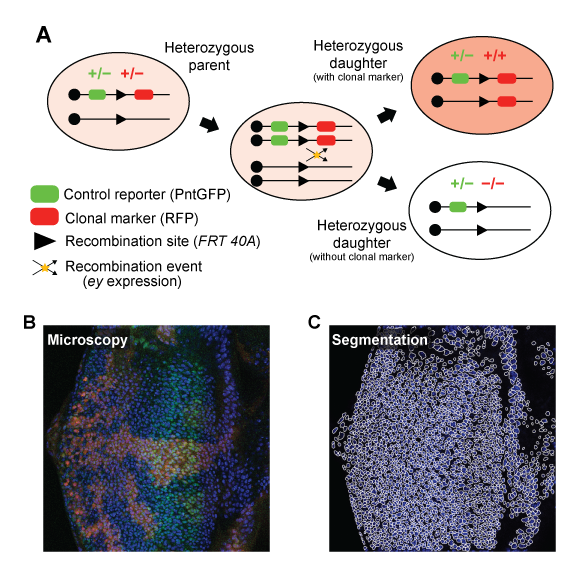
\includegraphics[width=0.95\columnwidth]{./figure_S1}
\caption[Example clones in the larval fly eye.]{\textbf{Example clones in the larval fly eye.} (A) Genetic schema for a bleedthrough control experiment. Red and green ovals represent genes encoding a RFP-tagged clonal marker and a GFP-tagged control reporter, respectively. Black lines depict a genomic locus. Recombination does not affect gene dosage of the control reporter, so GFP variation across clones is attributed to fluorescence bleedthrough. (B) Confocal image of an eye imaginal disc. Red, green, and blue reflect clonal marker, control reporter, and nuclear stain fluorescence, respectively. (C) Segmentation of the DAPI nuclear stain. White lines show individual segments.}
\label{fig:clones:figS1}
\end{figure}

\section{Image segmentation and quantification of nuclear fluorescence levels}
\label{ch:clones:segmentation}

We implemented a segmentation strategy based upon a standard watershed approach \cite{VanderWalt2014}. Briefly, we construct a foreground mask by Otsu thresholding the nuclear stain image following a series of smoothing and contrast-limited adaptive histogram equalization operations \cite{NobuyukiOtsu1979,VanderWalt2014}. We then apply a Euclidean distance transform to the foreground mask, identify the local maxima, and use them as seeds for watershed segmentation. When applied to the microscopy data, few visible spots in the nuclear stain were neglected, and the vast majority of segments outlined individual nuclei (Fig. \ref{fig:clones:figS1}C).

This approach is flexible and should perform adequately in many scenarios. However, we acknowledge that no individual strategy can address all microscopy data because segmentation is strongly context dependent. All subsequent stages of analysis were therefore designed to be compatible with any data that conform to our standardized file structure. This modular arrangement grants users the freedom to use one of the many other available segmentation platforms \cite{Bugarski2014}, including FlyEye Silhouette \cite{Pelaez2015a}, before applying the remaining functionalities of our framework. Regardless of how nuclear contours are identified, averaging the pixel intensities within them yields fluorescence intensity measurements for each reporter in each identified nucleus. We next sought to ensure that these measurements were suitable for comparison across clones.

\section{Bleedthrough correction}
\label{ch:clones:correction}

Despite efforts to select non-overlapping reporter bandwidths and excite them sequentially, it is not uncommon for reporters excited at one wavelength to emit some fluorescence in another channel (Fig. \ref{fig:clones:fig1b}B, yellow lines) \cite{Bacia2012,Zinchuk2007}. The end result is a positive correlation, or crosstalk, between the measured fluorescence intensities of two or more reporters. Exogenous correlations are problematic given that the purpose of the experiment is to detect changes in reporter levels with respect to the clonal marker.

In our microscopy data, individual clones were distinguished by their low, medium, or high expression levels of an RFP-tagged clonal marker (Fig. \ref{fig:clones:fig2}A). These images should not have shown any detectable difference in GFP levels across clones because all cells carried an equivalent dosage of the control reporter (Fig. \ref{fig:clones:figS1}A). However, the images visibly suffered from bleedthrough between the RFP and GFP channels (Fig. \ref{fig:clones:fig2}A,B). Bleedthrough was similarly evident when we compared measured GFP levels across labeled clones. Nuclei labeled mutant, heterozygous, or homozygous for the clonal marker had low, medium, and high expression levels of the control reporter, respectively (Fig. \ref{fig:clones:fig2}C, black boxes). The data were therefore ripe for systematic correction.

\begin{figure}[t]
\centering
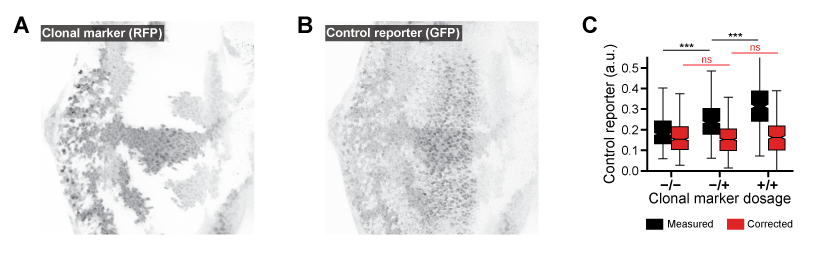
\includegraphics[scale=1.0]{./figure_2}
\caption[Automated correction of fluorescence bleedthrough in the larval eye.]{\textbf{Automated correction of fluorescence bleedthrough in the larval eye.} (A) Low, medium, and high expression levels of the RFP-tagged clonal marker. (B) GFP-tagged control reporter expression. RFP fluorescence bleedthrough is visually apparent upon comparison with A. (C) Comparison of control reporter expression between clones. Includes data aggregated across nine images taken from six separate eye discs. Data were limited to cells within the region of elevated GFP expression that were of approximately comparable developmental age (see Fig. \ref{fig:clones:figS2}E-G). Measurements are stratified by their assigned labels. Before correction, expression differs between clones (black boxes, $p<10^{-5}$). No difference is detected after correction (red boxes, $p>0.05$).}
\label{fig:clones:fig2}
\end{figure}

Spectral bleedthrough correction is common practice in other forms of cross-correlation and co-localization microscopy \cite{Bacia2012,Zinchuk2007}. These methods typically entail characterizing the extent of crosstalk between fluorophores globally \cite{Arsenovic2017,Kim2013}, on a pixel-by-pixel basis \cite{Elangovan2003}, or by experimental calibration \cite{Bacia2012}, then detrending all images or measurements prior to subsequent analysis. Our framework adopts the global approach, using the background pixels in each image to infer the extent of fluorescence bleedthrough across spectral channels.

\subsection{Statistical basis of bleedthrough correction}

Specifically, we assume the fluorescence intensity $F_{ij}$ for channel $i$ at pixel $j$ is a superposition of a background intensity $B_{ij}$ and some function of the expression level $E_{ij}$ that we seek to compare across cells \cite{McMullen2010}:
\begin{equation}
F_{ij} = B_{ij} + f(E_{ij})
\end{equation}
We further assume that the background intensity of a channel includes linear contributions from the fluorescence intensity of each of the other channels:
\begin{equation}
B_{ij} = \sum_{k \neq i}{\alpha_k F_{kj}} + \beta
\end{equation}
where $k$ is indexed over $K$ anticipated sources of bleedthrough. Given estimates for each $\{\alpha_1, \alpha_2, \ldots \alpha_K\}$ and $\beta$ we can then estimate the background intensity of each measurement:
\begin{equation} \label{eq:clones:bg_model}
\langle\ B_{ij}\ \rangle = \sum_{k \neq i}{\alpha_k \langle F_{kj} \rangle} + \beta
\end{equation}
where the braces denote the average across all pixels within a single nucleus. The corrected signal value is obtained by subtracting the background intensity from the measured fluorescence level:
\begin{equation} \label{eq:clones:correction}
\langle\ f(E_{ij}) \ \rangle = \langle\ F_{ij}\ \rangle - \langle\ B_{ij}\ \rangle
\end{equation}

Repeating this procedure for each nucleus facilitates comparison of relative expression levels across nuclei in the absence of bleedthrough effects. Bleedthrough correction performance is therefore strongly dependent upon accurate estimation of the bleedthrough contribution strengths, $\{\alpha_1, \alpha_2, \ldots \alpha_K\}$. 

\subsection{Characterization of fluorescence bleedthrough coefficients}
\label{ch:clones:model_fit}

We estimate these parameters by characterizing their impact on background pixels. For each image, we morphologically dilate the foreground until no features remain visible (Fig. \ref{fig:clones:figS2}A). We then extract the background pixels and resample them such that the distribution of pixel intensities is approximately uniform (Fig. \ref{fig:clones:figS2}B). Resampling helps mitigate the skewed distribution of pixel intensities found in the background. We then estimate values for each $\{\alpha_1, \alpha_2, \ldots \alpha_K\}$ and $\beta$ by fitting a generalized linear model to the fluorescence intensities of the resampled pixels (Fig. \ref{fig:clones:figS2}C). Each model is a variant of Equation \ref{eq:clones:bg_model} in which angled braces instead denote averages across all background pixels. We formulate these models with identity link functions under the assumption that residuals are gamma distributed. Their coefficients provide an estimate of the bleedthrough contribution strengths that may then be used to estimate the background fluorescence intensity of each nucleus in the corresponding image (Fig. \ref{fig:clones:figS2}D). The measurements may then be corrected through application of Equation \ref{eq:clones:correction}. 

We applied this procedure to the microscopy data, then compared measured control reporter expression across labeled clones. To mitigate edge effects, cells residing on the periphery of each clone were excluded from all comparisons (Fig. \ref{fig:clones:figS2}E). Border cells were identified by using a Delaunay triangulation to find all cells connected to a neighbor within a different clone. Our framework includes a simple graphical user interface that permits manual curation of which regions of the image field are included in subsequent analyses. We used this tool to limit our analysis to the region of elevated GFP expression near the morphogenetic furrow (Fig. \ref{fig:clones:figS2}F). Comparisons were further restricted to cells undergoing similar stages of development (Fig. \ref{fig:clones:figS2}G). These restrictions served to buffer against differences in developmental context and ensured that all compared cells were of similar developmental age. The remaining fluorescence measurements were then aggregated across all eye discs and compared between pairs of clones, confirming that bleedthrough correction successfully eliminated any detectable difference in GFP expression (Fig. \ref{fig:clones:fig2}C, red boxes, $p>0.05$ two-sided Mann-Whitney \textit{U} test).

\begin{figure}[h]
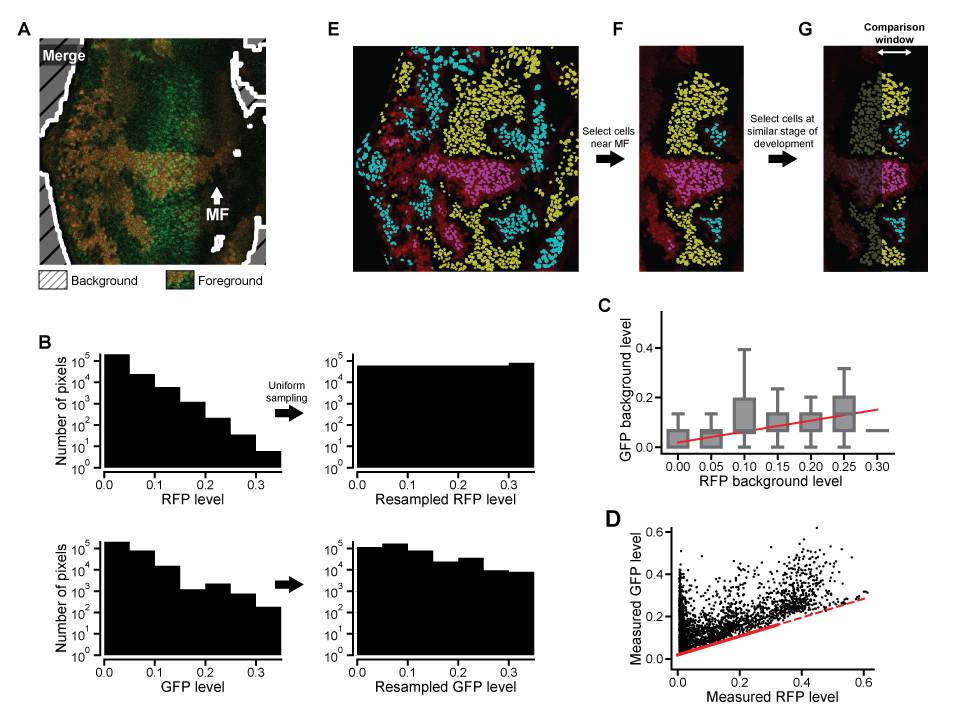
\includegraphics[scale=1.0]{./figure_S2}
\caption[Characterization of bleedthrough contribution strengths.]{\textbf{Using background pixels to characterize bleedthrough contributions in the foreground.} (A) Extraction of background pixels (striped region). Foreground includes the merged RFP and GFP images, surrounded by a white line. White arrow marks the morphogenetic furrow (MF). (B) Background pixel values are resampled such that RFP intensities are uniformly distributed. (C) A generalized linear model characterizes the contribution of RFP bleedthrough to GFP fluorescence. Boxes reflect windowed distributions of resampled background pixel intensities. Red line shows the model fit. (D) Measured GFP levels before bleedthrough correction. Markers represent individual nuclei. Red line shows the inferred contributions of RFP fluorescence bleedthrough. Dashed portion is extrapolated. (E-G) Data curation prior to statistical comparison of GFP levels. (E) Cells on the periphery of each clone are excluded. (F) The selection is limited to the region of elevated GFP expression near the MF. (G) It is further limited to cells of the same developmental age, defined by their relative positions along the x-axis.}
\label{fig:clones:figS2}
\end{figure}

\section{Automated annotation of clones}
\label{ch:clones:annotation}

Our annotation strategy seeks to label each identified cell as mutant, heterozygous, or homozygous for the clonal marker. Variation within each clone precludes accurate classification of a cell's genotype solely on the basis of its individual expression level. However, clonal lineages are unlikely to exist in isolation because recombination events are typically timed to generate large clones. Our strategy therefore integrates both clonal marker expression and spatial context to identify clusters of cells with locally homogeneous expression behavior, then maps each cluster to one of the possible labels. This unsupervised approach lends itself to automated annotation because the clusters are inferred directly from the data without any guidance from the user.

\subsection{Qualitative overview of clone annotation algorithm} 
\label{clones:methods:annotation}

We first train a statistical model to estimate the probability that a given measurement came from a cell carrying zero, one, or two copies of the clonal marker (Fig. \ref{fig:clones:figS3}A). This entails fitting a weighted mixture of three or more bivariate lognormal distributions (components) to a two dimensional set of observations (Fig. \ref{fig:clones:figS3}B,C). The first dimension corresponds to the clonal marker fluorescence level measured within each cell. The second dimension describes the local average expression level within the region surrounding each cell. We evaluate the latter by estimating a neighborhood radius from the decay of the radial correlation of the expression levels, then averaging the expression levels of all cells within that radius (Fig. \ref{fig:clones:figS3}D). The second dimension therefore measures the spatial context in which a cell resides. We balance model fidelity against overfitting by using the Bayesian information criterion to determine the optimal number of model components (Fig. \ref{fig:clones:figS3}E). We then cluster the components into three groups on the basis of their mean values (Fig. \ref{fig:clones:figS3}F), effectively mapping each component to one of the three possible gene dosages. The model may be trained using observations derived from a single image, or with a collection of observations derived from multiple images. Once trained, the model is able to predict the conditional probability that an individual observation belongs to one of the model's components, given its measured expression level.

\begin{figure}[h]
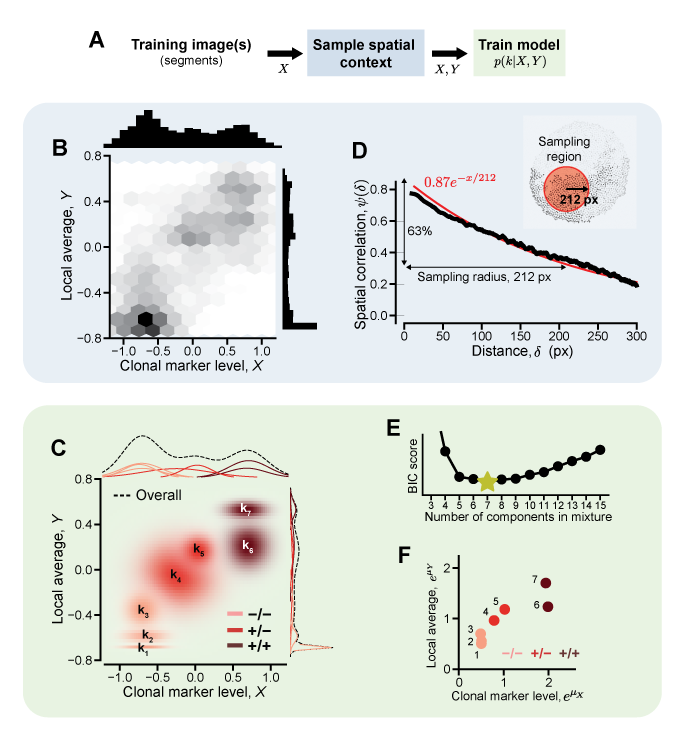
\includegraphics[scale=1.0]{./figure_S3}
\caption[Training a clone annotation model.]{\textbf{Training a clone annotation model.} (A) One or more images are segmented, yielding a set of fluorescence measurements $X$. These are used to sample the spatial context $Y$ of the neighborhood surrounding each cell. Both sets of values are used to train a mixture model. Subsequent panels demonstrate these procedures using the example shown in Figure \ref{fig:clones:figS3}C. (B) Expression levels are jointly distributed with the local average among neighboring cells. Center panel shows the joint distribution. Top and right bar plots show marginal distributions. (C) Mixture model identifies seven distinct components $k_i$. Center panel shows position and spread of each component. Top and right panels show marginal components scaled by their respective weights. Red shading denotes the label $m_i$ assigned to each component. The model predicts the posterior probabilities that a given sample $(X,Y)$ belongs to each component. (D) Neighborhood size is estimated by computing the decay constant of the spatial correlation function, $\psi(\delta)$. Black line shows the moving average of $\psi(\delta)$, red line shows an exponential fit. Inset shows the resultant sampling region. (E) The optimal number of mixture components is determined by minimizing BIC score. (F) Mixture components are labeled by k-means clustering their mean values. Markers reflect the component means, colors denote the assigned label.}
\label{fig:clones:figS3}
\end{figure}

We then use the learned conditional probabilities to detect entire clones, thus assigning a label to each cell. Rather than using the trained model to classify each observation, we compile a new set of observations by limiting each estimate of spatial context to spatially collocated communities with similar expression behavior (Fig. \ref{fig:clones:figS4}A). We identify these communities by applying a community detection algorithm to an undirected graph connecting adjacent cells (Fig. \ref{fig:clones:figS4}B). Edges in this graph are weighted by the similarity of clonal marker expression between neighbors, resulting in communities with similar expression levels (Fig. \ref{fig:clones:figS4}E, Steps I and II). The graph-based approach increases spatial resolution by limiting the information shared by dissimilar neighbors. Applying the mixture model yields an initial estimate of the probability that an observation belongs to one of the model's components (Fig. \ref{fig:clones:figS4}E, Step III). We further refine these estimates by allowing the probabilities estimated for each cell to diffuse throughout the graph (Fig. \ref{fig:clones:figS4}E, Step IV). The rate of diffusion between neighbors is determined by the weight of the edge that connects them, with more similar neighbors exerting stronger influence on each other. We then use the diffused probabilities to identify the most probable source component and label each observation (Fig. \ref{fig:clones:figS4}E, Step V). These probabilities also provide a measure of confidence in the assigned labels. We replace any low-confidence labels with alternate labels assigned using a marginal classifier that neglects spatial context (Fig. \ref{fig:clones:figS4}F,G), resulting in a fully labeled image (Fig. \ref{fig:clones:figS4}H).

\begin{figure}[t]
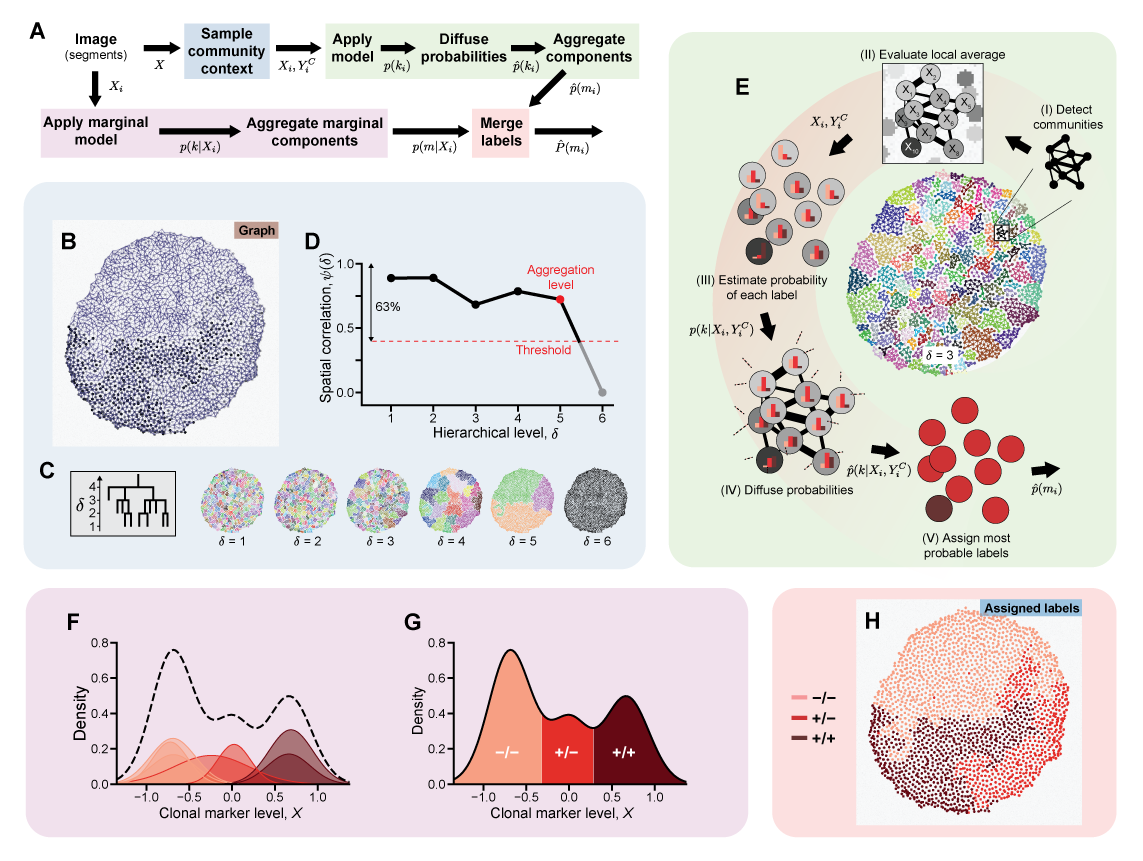
\includegraphics[width=1.0\columnwidth]{./figure_S4}
\caption[Label assignment using a trained clone annotation model.]{\textbf{Label assignment using a trained clone annotation model.}}
\label{fig:clones:figS4}
\end{figure}
\begin{figure}[h]
  \contcaption{(A) The measurements $X$ from a segmented image are used to sample the spatial context $Y^C$ of the community surrounding each cell before the mixture model is applied (blue and green path). They are simultaneously labeled using a marginal projection of the trained model (magenta path). The two sets of labels are then merged (red path). Subsequent panels demonstrate these procedures using the example shown in Figure \ref{fig:clones:figS3}C. (B-D) Spatial context sampling. (B) Weighted undirected graph connecting adjacent cells. Line thickness reflects the expression similarity between neighbors. (C) Community resolution is defined by aggregating clusters that fall below a cut level $\delta$ in the hierarchy. Images show potential levels of aggregation. Colors denote distinct communities. (D) Cut level is chosen by finding the maximum level (red dot) that remains lower than the decay constant of the spatial correlation function, $\psi(\delta)$ (black line). In this example, clusters are aggregated below the fifth level. Panel E instead depicts aggregation below the third level for ease of visualization. (E) Application of the mixture model. \emph{(I)} The graph connecting adjacent cells contains distinct communities of locally similar expression. \emph{(II)} Mean expression level within each community serves as the local average for each cell. \emph{(III)} Mixture model estimates the probability that each cell belongs to each of its component. Bar plots within each cell illustrate the cumulative probability of each label. \emph{(IV)} Posterior probabilities are diffused across the entire graph. \emph{(V)} Each cell is assigned its most probable label. (F,G) Application of a marginal mixture model that neglects spatial context. (F) Marginal mixture model components obtained by summing across the spatial context dimension of the full mixture model. Red shading denotes the label assigned to each component. Dashed black line is the overall marginal density. (G) Marginal classifier that labels cells strictly on the basis of their individual fluorescence level. Red shading denotes the most probable label for each expression level. (H) Annotated measurements. Red shading denotes the assigned label. Labels with low confidence $\hat{P}(m_i)<0.8$ are replaced by their marginal counterparts.}
\end{figure}

The algorithm leverages the collective wisdom of neighboring measurements to override spatially isolated fluctuations in clonal marker expression, and thereby enforces consistent annotation within contiguous regions of the image field. The size of these regions depends upon the granularity of estimates for the spatial context surrounding each cell. We used an unsupervised approach to choose an appropriate spatial resolution in a principled manner. In short, the resolution is matched to the approximate length scale over which expression levels remain correlated among cells. Both the training and application stages of our annotation algorithm use this automated approach (Figs. \ref{fig:clones:figS3}D and \ref{fig:clones:figS4}D), thus averting any need for user input.

\subsection{Statistical basis of clone annotation} 
\label{clones:methods:annotation_math}

We assume the measured fluorescence level $x_i$ for cell $i$ is sampled from an underlying distribution $p_m(x)$ for cells carrying $m$ copies of the gene encoding the clonal marker:
\begin{equation}
x_i \sim p_m(x)
\end{equation}
We further assume that $p_m(x)$ is comprised of a mixture of one or more lognormal distributions:
\begin{equation}
p_m(ln\ x) = \sum^{N}_{n=1}\lambda_n \mathcal{N}(ln\ x|\theta_{n})
\end{equation}
\begin{equation}
\sum^{N}_{n=1}\lambda_n=1
\end{equation}
where $0 \leq \lambda \leq 1$ are the mixing proportions, $\theta_n=(\mu_n,\sigma_n^2)$ are the mean and variance of the $n$th distribution. This assumption is supported by both empirical observations and theoretical insights \cite{Furusawa2005,Beal2017}. By superposition, the global distribution of measured fluorescence levels $p(ln x)$ for all values of $m$ are also sampled from a mixture of $K$ components:
\begin{equation}
p(ln\ x) =  \sum^{2}_{m=0} \alpha_m p_m(ln\ x) = \sum^{2}_{m=0} \alpha_m 
\sum^{N}_{n=1}\lambda_n \mathcal{N}(ln\ x|\theta_{n}) = \sum^{K}_{k=1}\lambda_k \mathcal{N}(ln\ x|\theta_{k})
\end{equation}
\begin{equation}
\sum^{K}_{k=1}\lambda_k=1
\end{equation}
where $\alpha_m$ denotes the overall fraction of cells with $m$ copies of the gene encoding the clonal marker. For brevity, we substitute $X = ln x$ yielding:
\begin{equation}
p(X) = \sum^{K}_{k=1}\lambda_k \mathcal{N}(X|\theta_{k})
\end{equation}

Given a collection of sampled fluorescence levels, $\{X_i\}_{i=1 \ldots N}$, we use expectation maximization to find values of $\theta_k$ and $\lambda_k$ for each of the model's $K$ components that maximize the log-likelihood of the observed sample. We repeat this procedure for a range of sequential values of $K$, resulting in multiple models of increasing size. We then balance model resolution against overfitting by selecting the model that yields the smallest value of the Bayesian Information Criterion (BIC):
\begin{equation}
BIC(K) = ln(N)q_K - 2 ln(\hat{L}_K)
\end{equation}
\begin{equation}
q_K = K-1 + 2^K
\end{equation}
where $N$ is the sample size, $ln(\hat{L})_K$ is the maximum value of the log-likelihood, the subscript $K$ denotes the number of mixture components in the model, and $q_K$ is the total number of parameters (i.e. $K-1$ values of $\lambda_k$ and $2^K$ values of $\mu_k$ and $\sigma_k^2$).

Applying Bayes' rule to the selected model infers the posterior probabilities that each sample $X_i$ belongs to the $k$th component:
\begin{equation}
p(k|X_i) = \frac{p(X_i | k) p(k)}{p(X_i)} = \frac{p(X_i | k) \lambda_k}{p(X_i)}
\end{equation}
where $p(X_i \mid k)$ is evaluated using the model's likelihood function and $p(X_i)$ is evaluated by marginalizing across each of the model's $K$ components. The end result is a mixture model that allows us to predict the probability that a given measurement of clonal marker expression belongs to a particular one of its component distributions.

We then define a many-to-one mapping, $f$, from each of the $K$ components of the mixture to each of the three possible values of $m$:
\begin{equation}
f: \{0,1,...K\} \to \{0,1,2\}
\end{equation}
We determine the mapping by k-means clustering the $K$ component distributions into three groups on the basis of their mean values, $e^{\mu_k}$. We may then assign a genotype label $m$ to each measurement $X_i$ by predicting the component $k$ from which it was sampled. The accuracy of these labels depends upon how closely the fitted mixture model reflects the true partitioning of gene copies among clones. While finite mixtures are always identifiable given a sufficiently large sample \cite{Teicher1963}, the algorithm used to fit the mixture tends toward local maxima of the likelihood function when the true components are similar (Wu, 1983). An approach based on a univariate mixture is thus inherently prone to failure when expression levels extensively overlap across clones, as variation within each clone precludes accurate classification of a cell's genotype solely on the basis of its individual expression level. However, clonal lineages are unlikely to exist in isolation because recombination events are usually timed to generate large clones. Our strategy therefore integrates both clonal marker expression and spatial context to identify clusters of cells with locally homogeneous expression behavior.

We incorporate spatial context by introducing a second jointly-distributed variable $Y_i$:
\begin{equation}
Y_i = \frac{1}{M_i} \sum^{M_i}_{j=0} X_j
\end{equation}
where the subscript $j$ indexes all $M_i$ neighbors of cell $i$. The new variable reflects the average expression level among the neighbors surrounding each cell. We define neighbors as pairs of cells located within a critical distance of each other. This distance, or sampling radius, is derived from the approximate length scale over which cells retain approximately similar clonal marker expression levels. Specifically, we determine the exponential decay constant of the spatial correlation function, $\psi (\delta)$:
\begin{equation}
\psi(\delta) = \frac {<( X_i -\mu_{X})( X_j -\mu_{X})>_{i,j \in \delta}} {\sigma_X^2}
\end{equation}
where $\mu_X$ and $\sigma_X^2$ are the global mean and standard deviation, and angled brackets denote the mean across all pairs of cells separated by distance $\delta$. We efficiently implement this procedure by fitting an exponential decay function to the down-sampled moving average of $\psi (\delta)$ as a function of increasing separation distance.

Following the introduction of spatial context, the mixture model becomes:
\begin{equation}
\label{eq:clones:bivariate_mixture}
p(X, Y) = \sum^{K}_{k=1}\lambda_k \mathcal{N}( X,Y |\theta_{k})
\end{equation}
where $\theta_{k} = (\vec{\mu}_{k},\vec{\sigma}_{k}^2)$ contains the mean and variance of each component given by vectors of length two. This formulation constrains each component's covariance matrix to be diagonal. The posterior is now:
\begin{equation}
p(k| X_i,Y_i) = \frac{p(X_i, Y_i | k) \lambda_k}{p(X_i, Y_i)}
\end{equation}
We can recover the univariate model by marginalizing the posterior over all values of $Y$:
\begin{equation}
p(k| X_i) = \sum_{j} p(k| X_i,Y_j)
\end{equation}
When neglecting spatial context, we use this expression to classify each sample by applying the mapping $f$ to the value of $k$ that maximizes $p(k \mid X_i)$:
\begin{equation}
f(\argmax_{k} p(k | X_i))
\end{equation}

In all other cases, we deploy a graph-based approach to refine the estimate of $p(k \mid X_i,Y_i)$. This first entails constructing an undirected graph connecting adjacent cells within each image. We obtain the graph's edges through Delaunay triangulation of the measured cell positions, then exclude distant neighbors by thresholding the edge lengths. Each edge is assigned a weight $w_{ij}$ reflecting the similarity of clonal marker expression between adjacent cells $i$ and $j$:
\begin{equation}
w_{ij} = exp \big( \frac{-E_{ij}}{\langle E \rangle} \big)
\end{equation}
\begin{equation}
E_{ij} = | X_i - X_j | 
\end{equation}
where $E_{ij}$ is the absolute log fold-change in measured expression level and angled brackets denote the mean across all edges. We chose an exponential formulation because it yields an approximately uniform distribution of edge weights. We then detect communities within the graph using the Infomap algorithm \cite{Rosvall2009}. The algorithm provides a hierarchical partitioning of nodes into non-overlapping clusters. We aggregate all clusters below a critical level that is again chosen by estimating the spatial correlation decay constant. We then enumerate $p(k \mid X_i,Y_i^c)$ where $Y_i^c$ is the spatial context obtained by averaging expression levels among all neighbors in the same community as cell $i$.

We further incorporate spatial context by allowing the posterior probabilities $p(k \mid X_i,Y_i^c)$ to diffuse among adjacent cells. We define the modified posterior probability $\hat{p}(k \mid X_i,Y_i^c)$ through a recursive relation analogous to the Katz centrality \cite{Katz1953}, initialized by $p(k \mid X_i,Y_i^c)$:
\begin{equation}
\hat{p}(k \mid X_i, Y^c_i) = \alpha \sum_{j}{w_{ij} \hat{p}(k \mid X_i, Y^c _i)} + \beta
\end{equation}
\begin{equation}
\beta = (1-\alpha) p(k| X_i,Y^c_i)
\end{equation}
where $\alpha$ is the attenuation factor and $w_{ij}$ are the edge weights. Expressed in matrix form, the solution for $\hat{p}(k \mid X,Y^c)$ is given by:
\begin{equation}
\hat{p}(k \mid X,Y^c) = ( I - \alpha W )^{-1} (1-\alpha)p(k \mid X, Y^c)
\end{equation}
where $I$ denotes the identity matrix and $W$ is the matrix of edge weights $w_{ij}$. We then assign a label to each measurement $X_i$ by applying $f$ to the value of $k$ that maximizes $\hat{p}(k \mid X_i,Y_i^c)$:
\begin{equation}
f(\argmax_{k} \hat{p}(k | X_i, Y^c_i))
\end{equation}

Finally, we assess the total posterior probability of each assigned label, $\hat{P}(m_i)$:
\begin{equation}
\hat{P}(m_i) = \sum_{ \mathclap{ \{ k | f(k)=m_i \}} } \hat{p}(k | X_i,Y^c_i)
\end{equation}
This measure reflects the overall confidence that $m_i$ is the appropriate label. Labels whose confidence falls below 80\% are replaced by their counterparts estimated using the marginal classifier. This substitution helps preserve classification accuracy in situations where spatial context is not informative, and is particularly useful when the annotated clones are relatively small.

\section{Manual assessment of annotation performance}

We sought to validate the performance of the annotation algorithm by assessing its ability to accurately label a dataset in which the true labels are known. While it is common practice to use human-labeled data as the gold standard, manually assigned labels do not represent a reliable and reproducible ground truth. Furthermore, we contend that validation with manually-labeled data entrains implicit human biases in the selection of performant algorithms. These biases are particularly pronounced in biological image data where intrinsic variation, measurement noise, and transient processes can make cell-type annotation a highly subjective, and thus irreproducible, task. 

Nevertheless, we begrudgingly labeled nuclei in each eye imaginal disc as mutant, heterozygous, or homozygous for the clonal marker, then automatically labeled the same cells (Fig. \ref{fig:clones:fig3}A). The two sets of labels showed strong overall agreement (Figs. \ref{fig:clones:fig3}B and \ref{fig:clones:figS5}A). Excluding cells on the border of each clone revealed greater than 97\% agreement in seven of the nine annotated images (Fig. \ref{fig:clones:figS5}B). Upon secondary inspection of the sole instance of substantial disagreement (Fig. \ref{fig:clones:figS5}C), we are unable to confidently discern which set of labels are more accurate.

\begin{figure}[t]
\centering
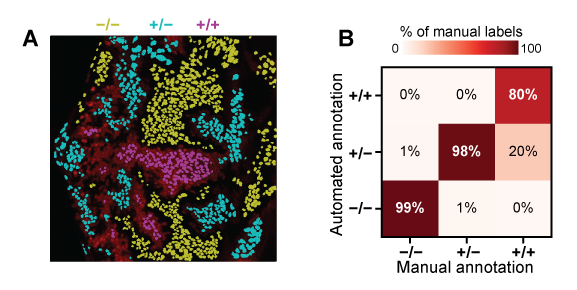
\includegraphics[scale=1.0]{./figure_3}
\caption[Automated unsupervised annotation of clones in the larval eye.]{\textbf{Automated unsupervised annotation of clones in the larval eye.} (A) Labels assigned by automated annotation. Yellow, cyan, and magenta denote the label assigned to each contour. Labels are overlayed on the RFP channel of the image shown in \ref{fig:clones:figS1}B. Cells on the periphery of each clone are excluded. (B) Comparison of automated annotation with manually-assigned labels. Confusion matrix includes data aggregated across nine images taken from six separate eye discs. Cells on the periphery of each clone are included. Columns sum to one.}
\label{fig:clones:fig3}
\end{figure}

\begin{figure}[h]
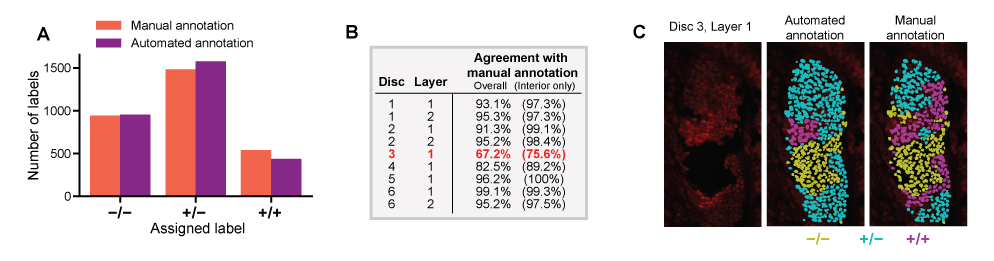
\includegraphics[scale=1.0]{./figure_S5}
\caption[Comparison of automated annotation with manually assigned labels.]{\textbf{Comparison of automated annotation with manually assigned labels.} (A) Distribution of labels among each possible value. (B) Agreement between automated and manual annotation. Values in parentheses exclude cells on the periphery of each clone. The sole instance of low agreement is marked in red. (C) Visual comparison of the instance in which automated and manual annotation differ. Image shows clonal marker fluorescence, overlayed colors denote the assigned label.}
\label{fig:clones:figS5}
\end{figure}

Synthetic benchmarking provides a powerful alternative to validation against manually labeled data. The idea is simple; measure how accurately an algorithm is able to label synthetic data for which the labels are known. The synthetic data generation procedure may be modeled after the process underlying formation of the real data, providing a means to assess the performance of an algorithm across the range of conditions that it is likely to encounter. The strategy therefore provides a means to survey the breadth of biologically plausible conditions under which the algorithm provides adequate performance. Synthetic benchmarking also facilitates unbiased comparison of competing algorithms, resulting in a reliable standard that may be called upon at any time. We therefore developed a platform to generate synthetic microscopy data that could be used to benchmark the performance of our annotation algorithm. 

\section{Generation of synthetic microscopy data}
\label{clones:data_generation}

Each synthetic dataset depicts a culture of cells distributed roughly uniformly in space. To generate each culture, we simulated the two dimensional growth of a population seeded with a single cell. Growth proceeds through sequential division of cells (Fig. \ref{fig:clones:figS6}A). Not all cells divide at each time-step because cell division is a stochastic process. Instead, each cell divides stochastically with a rate controlled by a global growth rate parameter.

Cells in this culture carry a gene encoding a clonal marker (Fig. \ref{fig:clones:figS6}B). During growth, the gene is subject to mitotic recombination (Fig. \ref{fig:clones:figS6}C). Each time a cell divides, its genes are duplicated and equally partitioned between the two daughter cells. However, in some instances a heterozygous parent may instead partition its two duplicate genes unequally, with one daughter receiving both and the other receiving none. These mitotic recombination events occur stochastically with a frequency defined by a global recombination rate parameter. 

After each round of cell division, all cells are repositioned in order to preserve approximately uniform spatial density (Fig. \ref{fig:clones:figS6}C). Repositioning is achieved by equilibrating a network of springs connecting each cell with its neighbors. This undirected network is constructed through Delaunay triangulation of all cells spatial positions. Edges on the periphery of the culture are systematically excluded by establishing a maximum polar angle between neighbors. This filtration removes spurious edges between distant pairs of cells. Edges connecting pairs of cells with the same clonal marker dosage are assigned a 10\% higher spring constant than edges that connect dissimilar cells. This modest bias ensures that cells tend to remain proximal to their clonal lineages. Cell positions are then updated using a force-directed graph drawing algorithm \cite{Kamada1989}. Alternating cell division and repositioning steps are then repeated until a predefined population size is reached. 

The timing and duration of recombination events affects the number and size of the resultant clones. In real experiments, recombination events are restricted to a particular stage of the developmental program through localized exogenous expression of the recombination machinery. We incorporated this feature into our cell growth simulations via two adjustable parameters. The first determines the minimum population size at which recombination may begin, while the second determines the number of generations over which recombination may continue to occur. These two parameters provide a means to tune the average number and size of clonal subpopulations in the synthetic data (Fig. \ref{fig:clones:figS6}D). Early recombination events generally entail larger clones, while shorter recombination periods limit the extent of clone formation (Fig. \ref{fig:clones:figS6}E).

\begin{figure}[h]
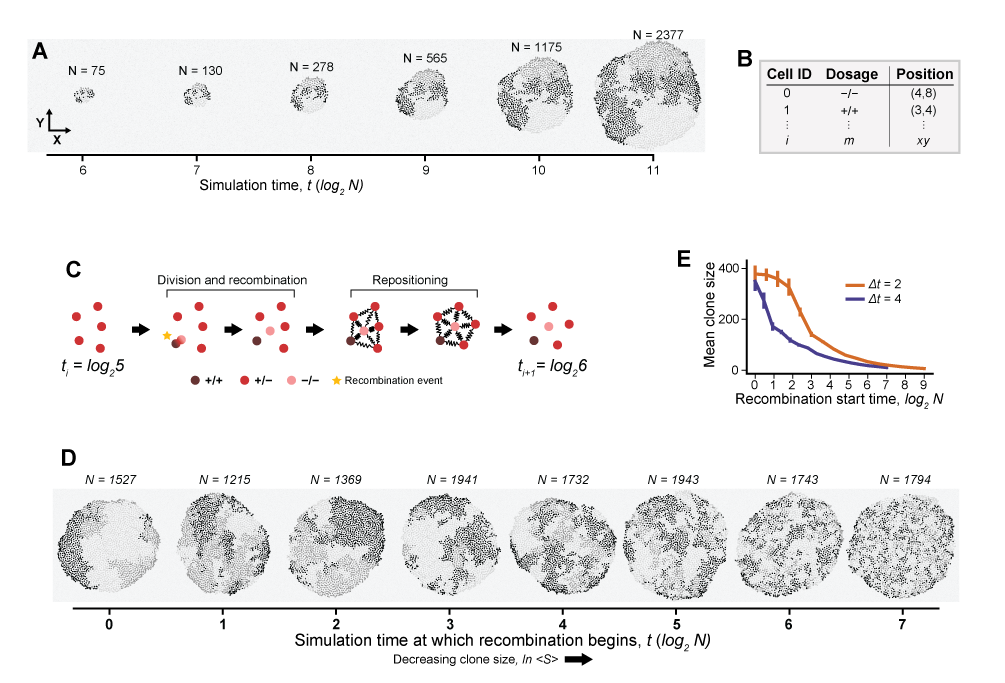
\includegraphics[width=1.0\columnwidth]{./figure_S6}
\caption[Simulated growth of a synthetic cell culture.]{\textbf{Simulated growth of a synthetic cell culture.} (A) Partial simulation time course. Each marker depicts a cell. Greyscale intensity reflects clonal marker gene dosage. Simulation time reflects the approximate number of cell divisions since the initial seed. (B) Simulations yield gene dosages and spatial coordinates for each cell. (C) Single iteration of an example simulation. Circles represent individual cells, red shading denotes clonal marker dosage. Cycles of cell division, recombination, and repositioning are repeated until the simulation reaches a specified end time ($t>11$ in panel A). (D) Cultures simulated with varying recombination start times. All cultures were subject to four generations of recombination ($\delta t=4$). Recombination start time increases from left to right. Later recombination events generally yield smaller clones. (E) Mean clone size (cells per clone) as a function of the recombination start time. Colors denote recombination period duration. Error bars reflect standard error of the mean across 50 replicates. Clone size generally decreases as recombination is limited to later times.}
\label{fig:clones:figS6}
\end{figure}

Each simulation yields a list of spatial coordinates and gene dosages for each nucleus (Fig. \ref{fig:clones:figS6}B). We generated a synthetic measurement for each nucleus by randomly sampling its fluorescence level in a dosage-depend manner. Specifically, the measured fluorescence levels $\{x_1, x_2, \ldots x_{i=N} \}$ were sampled from a lognormal distribution conditioned upon the corresponding gene dosage (Fig. \ref{fig:clones:figS7}A-C):
\begin{equation}
ln\ x \sim \mathcal{N}_n(\theta _n)
\end{equation}
where the subscript $n$ denotes the gene copy number and $\theta_n = (\mu_n,\sigma_{\alpha}^2)$ are the mean and variance of the corresponding distribution. We define $\mu_n$ such that the mean fluorescence level doubles for each additional copy of the gene:
\begin{equation}
\mu_{n } = ln(2^{n-1})
\end{equation}
We refer to $\sigma_{\alpha}$ as the \emph{fluorescence ambiguity} because it modulates the similarity of fluorescence levels across gene dosages. Increasing $\sigma_{\alpha}$ increases the overlap among $\mathcal{N}_0$, $\mathcal{N}_1$, and $\mathcal{N}_2$ (Fig. \ref{fig:clones:figS7}D,E), and consequently increases the difficulty of the annotation task (Fig. \ref{fig:clones:figS7}F).

\begin{figure}[h]
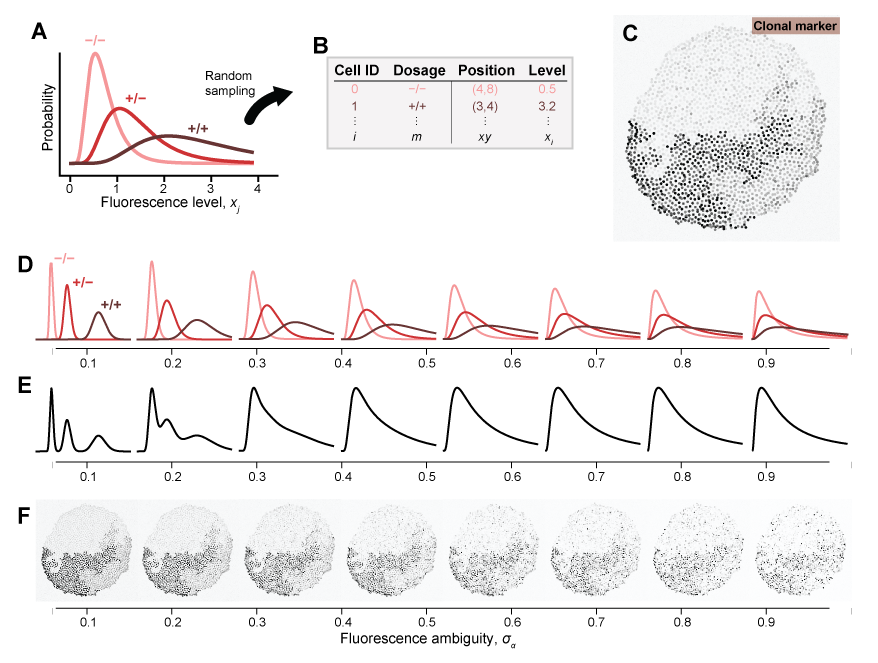
\includegraphics[width=1.0\columnwidth]{./figure_S7}
\caption[Tunable generation of synthetic microscopy data.]{\textbf{Tunable generation of synthetic microscopy data.} (A) Fluorescence levels are sampled from lognormal distributions conditioned upon gene dosage. (B) Synthetic data include a measured fluorescence level for each reporter in each cell. Text color reflects the generative distribution in A. (C) Synthetic image of clonal marker fluorescence when $\sigma_{\alpha}=0.25$. Each nucleus is shaded in accordance with its sampled fluorescence intensity. (D-F) Left to right, increasing the fluorescence ambiguity parameter broadens the overlap in fluorescence levels across gene dosages. (D) Distributions used to generate clonal marker fluorescence levels. Red shading denotes gene dosage. (E) Evenly weighted sum of the generative distributions. (F) Example images of clonal marker fluorescence.}
\label{fig:clones:figS7}
\end{figure}

\section{Synthetic benchmarking of annotation performance}
\label{ch:clones:benchmarking}

We generated a large synthetic dataset spanning a broad range of sixteen different clone sizes and fluorescence ambiguities (Figs. \ref{fig:clones:figS6}D and \ref{fig:clones:figS7}F, only half are shown for each). We performed 50 replicate simulations for each condition. All simulations were terminated when the total population exceeded 2048 cells. We assigned each cell a 20\% probability of division upon each iteration, and each cell division event was accompanied by a 20\% chance of mitotic recombination. Parent cells containing zero or two copies of the recombined genes were ineligible for recombination, effectively sealing the genetic fates of their respective lineages. 

We then annotated each set of measurements, and compared the assigned labels with their true values. The mixture model given by Equation \ref{eq:clones:bivariate_mixture} was independently trained and applied to each replicate. Training a single model on all replicates yields modestly stronger performance on average (not shown), but also yields more variable variable results across the parameter space because all labels are dependent upon the outcome of a single expectation maximization routine. We used the mean absolute error (MAE) as a comparison metric because it provides a stable measure of accuracy for multiclass classification problems in which the labels are intrinsically ordered \cite{Gaudette2009}. In other words, it penalizes egregious misclassifications more severely than mild ones.

We observed very strong annotation performance for all cases in which $\sigma_{\alpha} \leq 0.3$ (Fig. \ref{fig:clones:fig4}A). Unsurprisingly, performance suffers as the difficulty of the classification problem is increased. As cells on the periphery of each clone were not excluded from these analyses, the observed metrics provide a lower bound on the performance that may be anticipated in practice. The same trends are evident when performance is graded strictly on accuracy (Fig. \ref{fig:clones:fig4}B).

\begin{figure}[t]
\centering
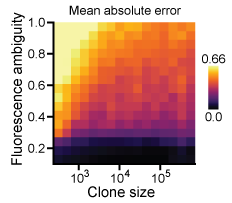
\includegraphics[scale=1.0]{./figure_4}
\captionsetup{width=.65\linewidth}
\caption[Synthetic benchmarking of automated annotation performance.]{\textbf{Synthetic benchmarking of automated annotation performance.} (A) MAE and (B) accuracy of the assigned labels. Each pixel reflects the average across 50 replicates. Clone size reflects the mean number of cells per clone. Accuracy denotes the fraction of cells that were correctly labeled. Performance improves with increasing clone size and worsens with increasing fluorescence ambiguity.}
\label{fig:clones:fig4}
\end{figure}

Performance improved with increasing clone size. We suspected this was caused by larger clones offering additional spatial context to inform the identify of each cell. We verified our assertion by re-evaluating performance relative to a variant of our annotation algorithm that neglects spatial context (Fig. \ref{fig:clones:figS4}G). As expected, the variant's performance exhibited no dependence on clone size (Fig. \ref{fig:clones:figS8}A). Comparing the two strategies confirmed that spatial context confers the most benefit when clones are large (Fig. \ref{fig:clones:figS8}B). Inclusion of spatial context also becomes increasingly advantageous as the fluorescence ambiguity is increased, even for smaller clones. Thus, spatial context adds progressively more value as the classification task becomes more difficult.

This observation may be rationalized from a statistical perspective. Each cell is classified by maximizing the probability that the assigned label is correct. We compute these probabilities using the estimated expression level of each cell. Neglecting spatial context, this estimate is limited to a single sample and is therefore highly sensitive to both measurement and biological noise. Incorporating spatial context expands the sample size and thereby reduces the standard error of the estimated fluorescence level. The strategy is thus generally well suited to scenarios in which fluorescence intensities correlate across large clones, and closely parallels computer vision methods that exploit spatial contiguity to segment image features with ill-defined borders \cite{Nguyen2012}. Because increased measurement precision comes at the expense of spatial resolution, we expect strong performance when measurements are aggregated across relatively large clones, but failure to detect small, heterogeneous clones. These expectations are consistent with the observed results. They are also conveniently aligned with the anticipated properties of real data, as experiments typically attempt to mitigate edge effects by driving early recombination events to generate large clones.

\begin{figure}[h]
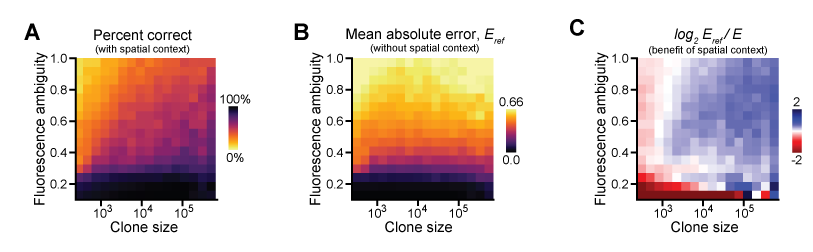
\includegraphics[scale=1]{./figure_S8}
\captionsetup{width=.65\linewidth}
\caption[Spatial context is most informative for large and ambiguous clones.]{\textbf{Spatial context is most informative for large clones with ambiguous fluorescence.}
(A) MAE of labels assigned using a marginal classifier that neglects spatial context. Performance worsens with increasing fluorescence ambiguity but does not depend upon clone size. (B) Annotation performance relative to the marginal classifier. Color scale reflects the $log_2$ fold-change in MAE when spatial context is neglected. Blue indicates that spatial context improves performance.}
\label{fig:clones:figS8}
\end{figure}

\section{Potential applications and continued development}

We used synthetic data to survey the performance of our annotation strategy across a much broader range of conditions than would have otherwise been possible with manually labeled data. This included conditions well beyond those of practical use. In particular, experiments designed to compare gene expression levels across clones would likely seek to avoid generating small clones with ambiguous clonal marker expression. Synthetic data provided a means to survey these edge cases and establish a lower bound on annotation performance. The strong performance observed across the remaining conditions bolsters our confidence that our annotation strategy is well suited to the images it is likely to encounter.

In each of our examples, clones were distinguished by ternary segregation of clonal marker fluorescence levels. Modern mosaic analysis techniques continue to deploy ternary labeling \cite{Gambis2011,Dourlen2013}, but also frequently opt for binary labeling of mutant versus non-mutant clones \cite{Fisher2017,Wu2007,Zhou2016} and dichromic labeling of twin-spots \cite{Heffern2009,Yu2010}. Our annotation scheme readily adapts to each of these scenarios provided that the number of anticipated labels is adjusted accordingly. In the case of dichromic labeling, binary classification would be performed separately for each color channel before merging the assigned labels. Extending the same logic to combinatorial pairs of colors suggests that our framework may also be compatible with multicolor labeling schemes used to simultaneously trace many clonal lineages over time \cite{Denes2013,Hadjieconomou2011,Hampel2011}. Our framework is thus well suited to many different mosaic analysis platforms deployed in the larval eye.

In principle, the framework described here should also be applicable to a wide variety of other tissues \cite{Neufeld1998,Tworoger1999} and model organisms \cite{Collins2010,Munoz-Jimenez2017,Wang2007} in which mosaics are studied. In practice, application to alternate contexts would require modifying some stages of the analysis. Most notably, image segmentation is strongly context dependent and any attempts to develop a universally successful strategy are likely to prove futile \cite{Meijering2012}. For this reason, we implemented a modular design in which each stage of analysis may be applied separately. For example, a user could perform their own segmentation before using our bleedthrough correction and clone annotation tools. By offering modular functionalities we hope to extend the utility of our software to the wider community of developmental biologists. Furthermore, the open-source nature of our framework supports continued development of more advanced features as various demands arise. Our synthetic benchmarking platform could then be used to objectively confirm the benefit conferred by any future developments.


\graphicspath{ {figures/ratio/} }

%CONTRIBUTIONS
%%%%%%%%%%%%%%%%%%%%%%%%%%%%%%%%%%%

\chapter{Ratiometric control of a transit to differentiation}
\label{ch:ratio}

A manuscript closely resembling this chapter was coauthored with Jean-Francois Boisclair Lachance, Nicol\'{a}s Pel\'{a}ez, Rachael Bakker, Heliodoro Navarro, Lu\'{i}s Amaral, Neda Bagheri, Ilaria Rebay, and Richard Carthew. A preprint is publicly available at \url{https://doi.org/10.1101/430744}.

Please note that all of the experiments detailed in this chapter were conceived, designed, and executed entirely by my colleagues. My personal contributions primarily include all of the computational analysis and modeling. I also produced all of the figures and wrote the majority of the text under the tutelage of Professor Richard Carthew.

%RATIO
%%%%%%%%%%%%%%%%%%%%%%%%%%%%%%%%%%%

\section{Transcription factors coordinate cell fate decisions}

Organismal development proceeds through a sequence of transitions that yield increasingly specific cellular states. Developmental programs employ a variety of strategies to coordinate transitions, ultimately ensuring that cells adopt the correct state in space and time. Elucidating these decision mechanisms is crucial to understanding the processes that guide development, as well as the diseases that arise when they fail.

How cells dynamically integrate the activities of one or more transcription factors to reliably execute state transitions is a long-standing question. Transcription factors initiate and enforce transitions by differentially regulating the expression of specific target genes \cite{Zheng1997,Ducy1997,McGhee2009}. Coordination among transcription factors can thus broaden the spectrum of possible cell responses to developmental cues \cite{ORiordan1999,Evans2003}. Positive and negative feedback can create bi-stable patterns of mutually exclusive transcription factor expression or activity that render state transitions irreversible \cite{Melen2005,Kueh2013,Yao2008,Park2012}. Cells can also regulate state transitions by differentially partitioning transcription factors between daughter cells \cite{Wolff2018}. In all of these models, mRNA and protein expression are believed to depend upon the absolute concentrations of the transcription factors involved \cite{Tontonoz1994,Laslo2006,Raj2010,Niwa2000}.

Studies of intercellular signaling suggest cells are capable of sensing relative levels of signaling molecules. For example, the TGF-$\beta$ pathway elicits a cell response following changes in input signaling relative to the preceding background \cite{Frick2017}. Fold-change, rather than absolute levels of $\beta$-catenin, dictate Wnt signal transduction in eukaryotic cells \cite{Goentoro2009a}. Likewise, aggregation of the social amoeba \textit{Dyctiostellium} depends on fold-change detection of extracellular cAMP concentrations \cite{Kamino2017}. Relative measurements can also involve multiple molecular components. In the BMP pathway, cells interpret multi-ligand inputs based on the relative levels of each ligand pair, with additive, differential, and ratiometric response types arising directly from the relative competition between different ligand-receptor pairs \cite{Antebi2017}. In yeast, pheromone response is insensitive to the absolute abundance of the G‐protein‐coupled receptor Ste2. Instead, cells respond to the fractional occupancy of the signal receptor by forming a ratiometric sensor between Ste2 and its regulatory inhibitor Sst2 \cite{Bush2016}. Topological features of molecular interaction networks, such as feed-forward loops, can also sense relative changes in molecule abundance \cite{Goentoro2009,Adler2018}. Combining such circuits with precise coordination of signaling inputs would yield a molecular decision mechanism that is robust to fluctuations in the abundance of participating molecules. Notably, while relevant transcription factors are precisely controlled during development \cite{Doe2017,Erclik2017}, it remains unknown whether cells sense the relative concentrations or activities of different transcription factors when executing cell state transitions.

Two ETS-domain transcription factors, the activator Pointed (Pnt) and the repressor Yan (also known as Anterior open, Aop), are essential regulators of cell fate transitions at numerous stages of \textit{Drosophila} development \cite{Gabay1996,Halfon2000,Morimoto1996,Xu2000,Flores2000}. Consistent with their opposing regulatory effects, genetic studies have shown that Pnt and Yan can act antagonistically in guiding numerous cell fate transitions \cite{Brunner1994,ONeill1994a,Gabay1996,Halfon2000}. The \textit{pnt} locus encodes two protein isoforms, PntP1 and PntP2, that differ in their N-terminal transactivation domains but share the same DNA-binding domain (Fig. \ref{fig:ratio:fig1}A) \cite{Klambt1993,Scholz1993}. Specifically, PntP1 is constitutively active whereas PntP2 requires phosphorylation via the RTK signaling pathway to become a potent activator \cite{ONeill1994a,Brunner1994}. Because both Pnt isoforms and Yan bind to a common ETS-binding DNA sequence motif GGA(A/T) \cite{Wei2010}, competition for occupancy and regulation of common target genes must be precisely orchestrated \cite{ONeill1994a,Halfon2000,Flores2000,Xu2000,Webber2013,Webber2013a,BoisclairLachance2018,Webber2018}.

Pnt and Yan display mutually exclusive expression patterns in several developing tissues \cite{BoisclairLachance2014}. The embryonic ventral ectoderm provides a classic example in which cells unambiguously reside in one of two stable states \cite{Gabay1996,Melen2005}. These and similar observations inspired a bistable switch model of cell fate specification in which the multipotent state is defined by high absolute Yan levels and the differentiated state is defined by high absolute Pnt levels \cite{Graham2010}. The model posits that RTK signaling triggers a transition from target gene repression to activation by degrading Yan and activating PntP2 \cite{Brunner1994,Rebay1995}. A positive feedback loop in which transient phosphorylation of PntP2 activates expression of \textit{pntP1} is thought to stabilize the transition by enabling prolonged signaling-independent stimulation of target genes \cite{Shwartz2013}. Sustained PntP1 expression in cells devoid of Yan thereby recapitulates a complementary expression pattern under the control of RTK signaling \cite{BoisclairLachance2014}. However, Pnt and Yan are also co-expressed during cell fate commitment in several developmental contexts \cite{BoisclairLachance2014}. For example, the two proteins are co-expressed in posterior follicle cells of the early egg chamber and throughout the embryonic mesoderm \cite{BoisclairLachance2014}, where they are required for specification of cell fates \cite{Morimoto1996,Halfon2000}. Co-expression also occurs in the larval eye \cite{BoisclairLachance2014}, despite the repeated use of RTK signaling to designate cell fates \cite{Freeman1996}. Eye development thus prompts exploration of how state transitions are resolved from concurrent Pnt and Yan expression in response to signaling cues.

Eye development is divided into two distinct phases, growth and differentiation. In the first phase, multipotent progenitor cells in the eye-field asynchronously proliferate from the earliest larval stage until the third instar stage of larval life \cite{Wolff1993}. The differentiation phase of eye development begins in the early third instar larva, when cells situated at the posterior margin of the eye disc start to differentiate into photoreceptor (R) cells, followed by progressively more anterior cells (Fig. \ref{fig:ratio:fig1}B). This wave of differentiation is initiated and coordinated by a morphogenetic furrow (MF), which traverses the eye disc from posterior to anterior for the remainder of the third instar stage up to the early pupal stage \cite{Voas2004}. Progenitor cells located immediately anterior to the MF arrest in G1 of the cell cycle and express a transcription factor called Atonal. Refinement of Atonal expression within this field establishes the differentiation program by specifying individual R8-type photoreceptors in a periodic pattern immediately posterior and parallel to the MF \cite{Jarman1994,Zhang2006}. Each R8 cell then locally secretes an RTK ligand that induces R8's multipotent neighbors to differentiate into other photoreceptor types (Fig. \ref{fig:ratio:fig1}C) \cite{Freeman1996,Voas2004}. Transitions sequentially occur approximately every two hours to form R2/R5, R3/R4, R1/R6, and R7 photoreceptors \cite{Wolff1993}. Many cells remain as multipotent progenitors even after all R cell fates have been adopted. These cells will adopt other fates at later stages of eye development, with any surplus eliminated by apoptosis \cite{Wolff1991}.

R cell fate specification violates three central tenets of the bistable switch model. First, Pnt and Yan do not exhibit a mutually exclusive expression pattern during eye development. The two proteins are extensively co-expressed in both progenitor and differentiating cells within and posterior to the MF \cite{BoisclairLachance2014}. Second, transitioning cells do not originate in a stable high Yan state. We recently quantified Yan protein dynamics during larval and early pupal eye development \cite{Pelaez2015a}. In progenitor cells, Yan displays pulsatile dynamics in which protein levels rapidly increase as the MF passes and then gradually decay back to low initial values. Third, transitioning cells do not adopt a stable high Pnt state. Visual inspection of eye discs carrying a fluorescent reporter for Pnt expression suggest that Pnt levels decay on a timescale comparable to Yan in transitioning cells \cite{BoisclairLachance2014}. Despite their similar expression patterns, the two proteins still exhibit antagonistic effects on R cell fate determination. Pnt stimulates progenitor cells to transit to an R cell fate while Yan inhibits these transitions \cite{ONeill1994a,Rebay1995}.

Here, we explore this apparent paradox to understand how two coexpressed transcription factors with comparable DNA binding specificity but opposing transcriptional functions elicit precisely controlled cell state transitions in the developing eye. We find that cell states are regulated by the relative abundance of these two proteins, rather than by their absolute concentrations. Progenitor cells dynamically maintain an approximately constant ratio of Pnt-to-Yan protein despite their absolute concentrations varying over time. Cells that transition to R cell fates rapidly increase their Pnt-to-Yan ratio, which remains elevated over time. We show that a ratio control strategy buffers this ratio against variable abundance of either protein. We also find that the signaling inputs of the Yan-Pnt network regulate the dynamics of the transcription factor ratio. Although Notch and Ras signals can both promote and inhibit differentiation in the developing eye \cite{Fortini1993,Freeman1996}, we find that Notch signaling predominantly decreases the Pnt-to-Yan ratio in progenitor cells while Ras signaling mainly increases the ratio. Notch and Ras signals thus inhibit and promote cell state transitions in the eye by dynamically tuning the ratio of the two transcription factors. We conclude that progenitor cells interpret an increase in the abundance of Pnt relative to Yan as a cue to differentiate.

\section{PntGFP expression dynamics in the developing eye }

Although Pnt expression has been qualitatively studied in the eye \cite{BoisclairLachance2014}, its dynamics have not been quantified. Therefore, we took advantage of a fully functional genomic transgene in which both \textit{pntP1} and \textit{pntP2} are C-terminally tagged with GFP. As previously reported \cite{BoisclairLachance2014}, \textit{pnt-gfp} rescues \textit{pnt} null mutants to viable, fertile adults with wild type external morphology (Fig. \ref{fig:ratio:figS1}A,B). Qualitative examination of Pnt-GFP expression in 100h eye-antennal imaginal discs revealed a region of very low expression in cells anterior to the MF, followed by strong expression in two parallel stripes of cells immediately posterior to the MF (Fig. \ref{fig:ratio:fig1}D, regions 1 and 2).

\begin{figure}[h!]
\centering
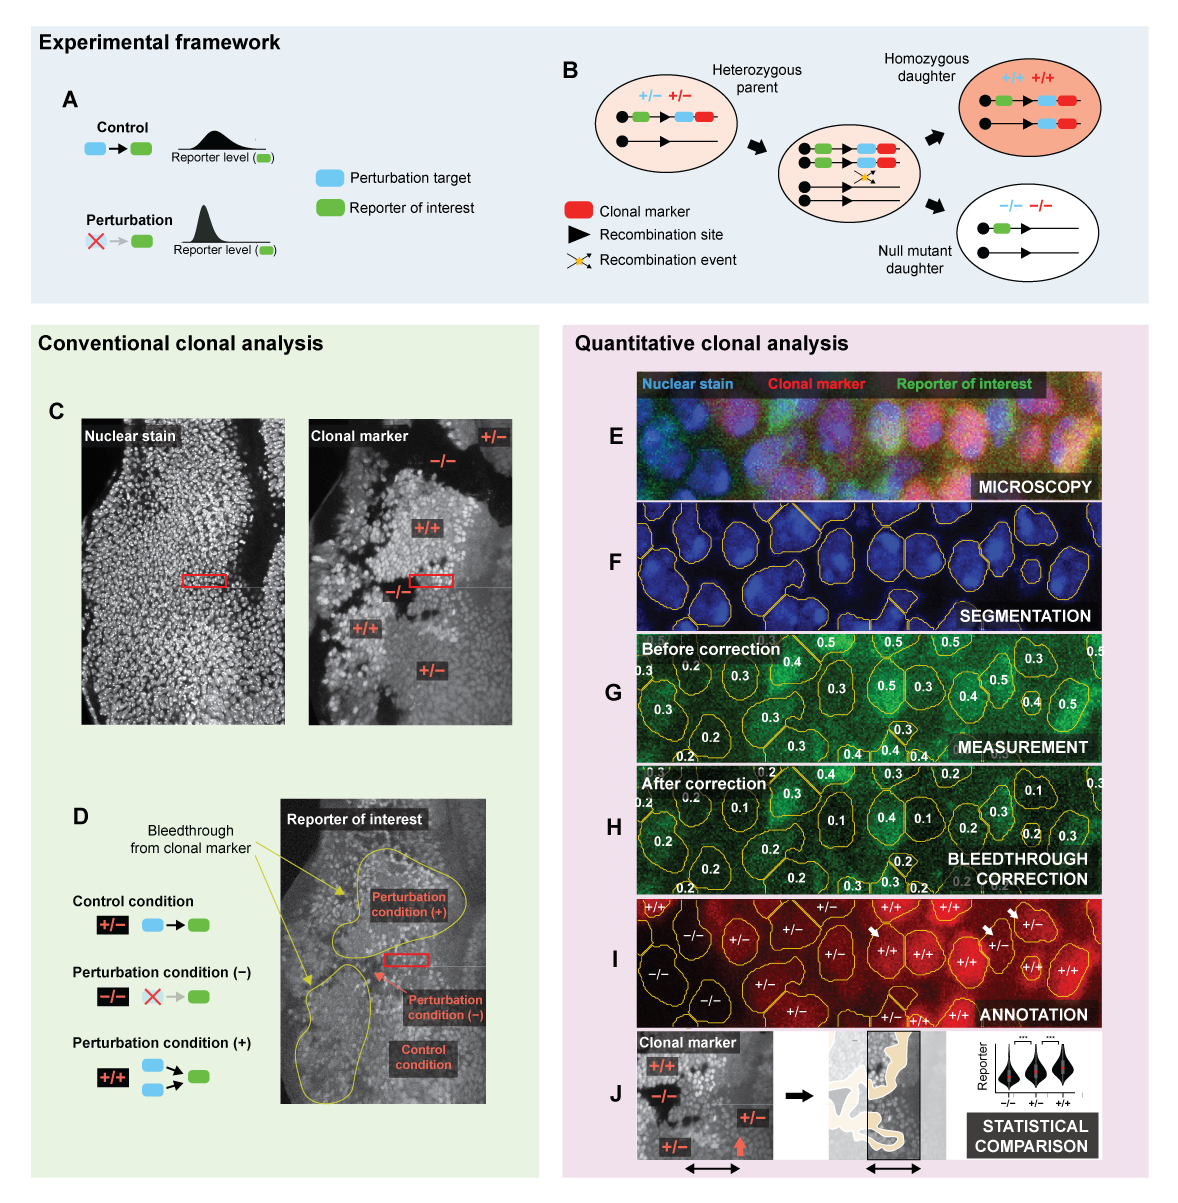
\includegraphics[width=1.0\columnwidth]{./figure_1}
\caption[Dynamics of Pnt and Yan expression during eye development.]{ (Continued on the next page.) }
\label{fig:ratio:fig1}
\end{figure}
\begin{figure}[h!]
\contcaption{\textbf{Dynamics of Pnt and Yan expression during eye development.} (A) Diagram of the \textit{pnt} locus encoding the Pnt-P1 and Pnt-P2 protein isoforms. The isoforms share an ETS DNA-binding domain (red) but are distinguished by the presence of a SAM domain (blue) within Pnt-P2. Green arrows at the C-termini depict insertion sites of GFP in the \textit{pnt-gfp} allele, black arrows at the N-termini depict insertion sites of the $pnt^{HS20}$ and $pnt^{1277}$ enhancer-trap alleles. Adapted from Shwartz et al. (2013). (B) Differentiation is initiated in the developing eye by the MF, which moves across the eye epithelium from posterior to anterior (white arrow). On the furrow's posterior side, G1-arrested progenitor cells differentiate (light blue). Formation of regularly spaced R8 photoreceptors (red dots) precedes recruitment of additional R cell types (yellow dots). On the anterior side, progenitor cells are still proliferating (dark blue). Axis refers to time elapsed since fertilization. Adapted from Pel\'{a}ez et al. (2015). (C) Top, cartoon of an apical view of the sequential differentiation of eight R cell types from multipotent progenitor cells (grey) and their relative positions within a single ommatidium. Arrows denote signals transmitted from the R8 to nearby cells. Bottom, a cross-section view through an eye disc, showing the epithelial constriction that marks the MF (boxed region) and then the relative nuclear positions of progenitors (grey) and specified R cells (various colors). Together, the stereotyped features depicted in this schematic enable unambiguous identification of each cell type as ommatidial assembly proceeds. Adapted from Pel\'{a}ez et al. (2015). (D) Maximum intensity projection of Pnt-GFP fluorescence in an imaginal disc fixed $\sim$ 100 h after fertilization. Right panel corresponds to the region enclosed by dashed white lines in the left panel. Morphogenetic furrow (orange arrow) precedes the first and second stripes of strong Pnt-GFP expression (black lines, labeled 1 and 2). (E) Pnt-GFP expression in progenitor cells. Grey points are individual cells, solid line is the smoothed moving average. Orange shading indicates the first and second stripes of Pnt-GFP expression. (F, G) R cell recruitment from the (F) first and (G) second pulses of Pnt-GFP expression. Solid lines and shaded regions denote moving averages and their 95\% confidence intervals. (H, I) Confocal images of (H) Pnt-P1 and (I) Pnt-P2 enhancer-trap co-expression with Pnt-GFP. Orientation is consistent with panel D. Morphogenetic furrow (orange arrow) precedes first and second stripes of Pnt-GFP induction (black lines, labeled 1 and 2). In merged images, Pnt-GFP is green and enhancer-trap expression is magenta. (J, K) Measured (J) Yan expression and (K) $log_2$-transformed Pnt-GFP to Yan ratios in progenitor cells. Grey points are individual cells, solid line is a smoothed moving average.}
\end{figure}

\section{The Pnt-to-Yan ratio varies between cells in different states }

We used Histone-RFP fluorescence from a His2Av-mRFP transgene to label all eye cell nuclei for automated segmentation following direct fluorescence microscopy of fixed specimens \cite{Pelaez2015a,Pelaez2016}. Average Pnt-GFP fluorescence levels and exact 3D positions were then calculated for all nuclei in each developing eye disc. Pnt-GFP fluorescence levels were normalized to Histone-RFP, which provided some control over measurement noise and nuclear constriction that occurs at the MF \cite{Pelaez2015a,Pelaez2016}. We mapped each cell's position along the anterior-posterior coordinate of the eye disc to a point in developmental time. This linear approximation is sufficiently accurate because the MF moves across the eye field with approximately constant velocity, forming one column of R8 cells every two hours \cite{Basler1989,Campos-Ortega1977}. The distance between a cell and the MF is therefore proportional to the time elapsed since the MF passed. We also manually assigned a state value to each cell. Cell state classification is possible because nuclei can be unambiguously identified without cell-specific markers by their morphology, apical-basal position, and relative distance to the furrow \cite{Ready1976a,Tomlinson1985,Tomlinson1987a,Wolff1993,Pelaez2015a,Pelaez2016}. Combined, these data allowed us to infer a macroscopic view of cell state transition dynamics from the spatial arrangement of cells relative to each other and the MF. Although our approach cannot measure the developmental progression of an individual cell, it provides a dynamic view of thousands of cells across a developing eye. From this information, average cell behaviors can be reconstructed and modeled.

Progenitor cells anterior to the MF expressed a basal level of Pnt-GFP, but expression dramatically increased in cells immediately anterior to the MF (Fig. \ref{fig:ratio:fig1}E). This was followed by two successive pulses of Pnt-GFP expression, marked by peaks where protein expression reached maximal amplitude. The pulses matched the visual stripes seen in regions 1 and 2 (Fig. \ref{fig:ratio:fig1}D). Thereafter, Pnt-GFP decayed to a low basal level. The two pulses of Pnt-GFP in progenitor cells coincided with the two periods of transition to R cell states (Figs. \ref{fig:ratio:fig1}F,G and \ref{fig:ratio:figS1}C). Transitions to R8, R2/R5, and R3/R4 states occurred during the first pulse, while transitions to R1/R6, and R7 states occurred during the second pulse.

Based on prior description of the distinct temporal expression patterns of isoform-specific \textit{pnt} transcriptional reporters \cite{Shwartz2013}, we suspected that each pulse of Pnt-GFP corresponded to the induction of either PntP1 or PntP2. Using flies that carried the \textit{pnt-gfp} transgene and either a \textit{pntP1-} or \textit{pntP2}-specific reporter, we found that region 1 overlapped with the domain of strongest \textit{pntP1} reporter expression, and region 2 corresponded to the domain of strongest \textit{pntP2} reporter expression (Fig. \ref{fig:ratio:fig1}H,I). Low levels of \textit{pntP2} reporter expression were detected in region 1 and low levels of \textit{pntP1} reporter were detected in region 2. Therefore, Pnt expression appears as a PntP1-PntP2 pulse sequence. The two groups of differentiating R cells predominantly expressed PntP1 or PntP2 respectively (data not shown, see \cite{Pelaez2016}), suggesting that specific Pnt isoforms are used to specify distinct cell fates.

All cell state transitions coincided with a rapid increase in Pnt-GFP (Fig. \ref{fig:ratio:fig1}F,G). The earliest identified R cells had, on average, 25-50\% higher levels of Pnt-GFP than progenitor cells at comparable times. Pnt-GFP then rapidly decayed in all differentiating R cells, with all but the R7 cell type exhibiting faster decay kinetics than progenitor cells. Thus, transitioning R cells did not adopt stable high Pnt levels as predicted by a bi-stable model of R cell fate specification. Rather, the measured Pnt-GFP expression dynamics were similar to those previously reported for Yan \cite{Pelaez2015a}. Average levels of both proteins increased as the MF passed, then decayed during cell state transitions. These similar population-wide dynamics led us to ask how cell states are resolved from the co-expression of two transcription factors with opposing transcriptional functions at the single cell level.

We explored this question by simultaneously measuring Pnt-GFP and Yan in each nucleus using an anti-Yan monoclonal antibody. Previously, we had shown that Yan dynamics measured with the antibody were almost identical to those measured by a YFP tagged version of Yan \cite{Pelaez2015a}, validating our approach. Pnt-GFP and Yan were induced at the same time in progenitor cells (Figs. \ref{fig:ratio:fig1}E,J and \ref{fig:ratio:figS1}D). Yan levels reached a maximum amplitude between the two pulses of Pnt-GFP. Yan then decayed back to a basal steady-state level, interrupted by a transient plateau during the second pulse of Pnt-GFP. Despite their alternating maxima, the overall induction and decay of Pnt-GFP and Yan were concurrent in progenitor cells.

The similar dynamics prompted us to consider whether relative levels of Pnt and Yan dictate cell state transitions in the eye. To explore this possibility, we measured the ratio of Pnt-to-Yan in each progenitor cell. Strikingly, the average Pnt-to-Yan ratio remained dynamically stable about a constant value over time (Fig. \ref{fig:ratio:fig1}K). However, from 0 to 15 h, there was considerable cell-to-cell heterogeneity in the ratio. Some cells had above-average ratios when they were expressing peak levels of Pnt-GFP, and many cells had below-average ratios when they were between the Pnt-GFP pulses. After the second pulse of Pnt-GFP expression, cells acquired a slight bias towards Yan. These are the progenitor cells that remain multipotent and are used to differentiate into other cell types later in development \cite{Wolff1991}. As the two positive spikes in the ratio coincided with the two periods of cell state transition, we reasoned that dynamic changes in the ratio might control the state of cells and regulate their transit to differentiation.

As a first test of this idea, we quantified the levels of Pnt-GFP and Yan in cells that had undergone R cell state transitions. We focused on R2/R5 and R1/R6 cells, since they are representative of transitions of cells derived from groups 1 and 2, respectively. As previously noted, Pnt-GFP levels were elevated in both sets of ``young'' R cells as soon as we could confidently identify them (Fig. \ref{fig:ratio:fig2}A,B). In contrast, Yan levels were lower in these young R cells than in progenitor cells of comparable age (Fig. \ref{fig:ratio:fig2}C,D). This meant that the average ratio of Pnt-to-Yan was elevated 1.5- to 2-fold in young R cells (Fig. \ref{fig:ratio:fig2}E,F). The ratio elevation was more modest in young R2/R5 cells than in young R1/R6 cells, but all increases were significant (KS test, $p<0.001$). The elevated ratio persisted for all times thereafter as differentiation proceeded. Analogous ratio trends were evident with the other R cell types as well (Figs. \ref{fig:ratio:fig2}G and \ref{fig:ratio:figS2}), suggesting that different state transitions share a common requirement for sustained change in the Pnt-to-Yan ratio relative to progenitor cells (Fig. \ref{fig:ratio:figS2}C-G).

\begin{figure}[h!]
\centering
\vspace{0pt}
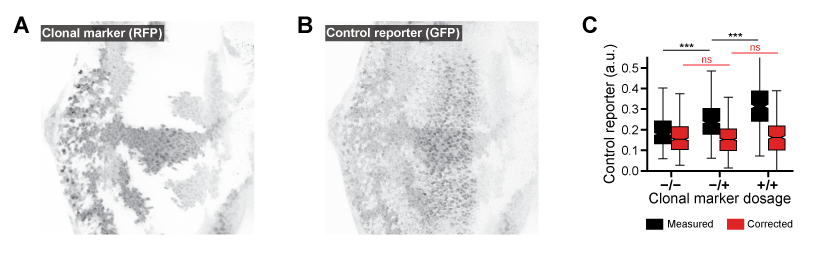
\includegraphics[width=1\columnwidth]{./figure_2}
\caption[Pnt-to-Yan ratios differ between cellular states.]{\textbf{Pnt-to-Yan ratios differ between cellular states.} (A-F) Measured (A, B) Pnt-GFP expression, (C, D) Yan expression, and (E, F) Pnt-GFP to Yan ratio dynamics in R2/R5 (blue) and R1/R6 (red) cells. Progenitors are grey. Solid lines are smoothed moving averages across 250 and 50 samples for progenitor and R cells, respectively. Yellow shading indicates time spanned by young R cells. (G) Comparison of Pnt-to-Yan ratio levels between young R cells (color filled boxes) and their concurrent progenitors (grey filled boxes). Colors denote R cell types. For each R cell type, the ten earliest identifiable R cells in each disc were designated as young R cells. Progenitor cells that fall within the time window spanned by these young R cells were designated as concurrent progenitors. Asterisks denote significance (KS 2-sample test, $p<0.001$). (H, I) Joint distributions of Pnt-GFP and Yan protein levels for young (H) R2/R5 and (I) R1/R6 cells. Progenitor cells concurrent with the corresponding young R cells are shown in grey. Black line denotes the median Pnt-to-Yan ratio among the progenitor cells shown.}
\label{fig:ratio:fig2}
\end{figure}

We next asked whether elevated Pnt-to-Yan ratios precede the onset of R cell state transitions. If R cells are recruited from a subpopulation of progenitors with relatively high ratios, some progenitors should exhibit ratios comparable to those of early R cells. We compared the distribution of Pnt-to-Yan ratios in young R cells versus concurrent progenitor cells (Fig. \ref{fig:ratio:fig2}H,I). The extensive overlap between the two populations implies that some cells we morphologically classified as progenitors were actually transitioning to R cell fates. Additionally, ratios may have increased among a subset of progenitors that did not ultimately transition to an R cell state. Many progenitors also adopted low Pnt-to-Yan ratios during this time period that did not overlap with the early R cell population. We reasoned that these cells were not viable candidates for recruitment, suggesting that the extent of variation in the ratio among progenitors constrains their competence for differentiation.

We then asked whether variation in the Pnt-to-Yan ratio strictly coincides with R cell fate transitions. We anticipated that variability should arise within the pool of progenitors from which R cells are recruited, then subside as fates are resolved. We previously reported methods to quantify the dynamic cell-to-cell heterogeneity of Yan concentration \cite{Pelaez2015a}. We applied similar analysis to simultaneously quantify the heterogeneity of Pnt, Yan, and the Pnt-to-Yan ratio among both progenitors and early R cells (Fig. \ref{fig:ratio:figS3}). A broad increase in variation of the ratio among progenitors coincided with the time periods in which state transitions occurred. Ratio variation was predominantly attributed to Yan and Pnt variability during the first and second groups of R cell state transitions, respectively. Heterogeneity among progenitors then decreased back to basal levels after all R cell fate transitions were complete. Similar trends were evident among transitioning R cells, but with a more rapid approach toward a consensus ratio following fate specification.

\begin{figure}[h]
\centering
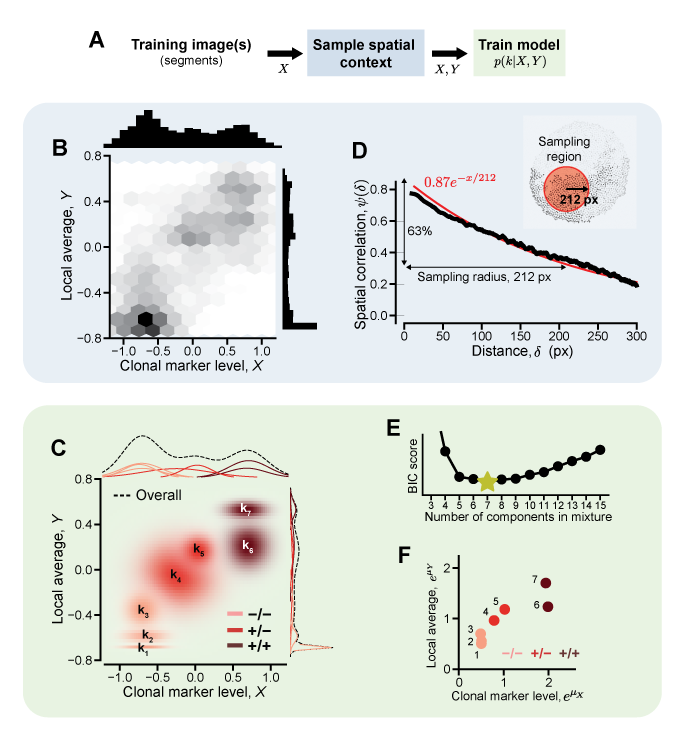
\includegraphics[width=1.0\columnwidth]{./figure_S3}
\caption[Dynamics of expression variability in progenitors and R cells.]{\textbf{Dynamics of expression variability in progenitor and R8, R2/R5 and R1/R6 cells.} Heterogeneities of (A) Pnt expression, (B) Yan expression, and (C) the $log_2$-transformed ratio are estimated by de-trending fluctuations about a moving average of 250 sequential cells. Lines are moving averages of 250 sequential fluctuations, shaded regions are bootstrapped 95\% confidence intervals for the moving average. Colors denote cell type.}
\label{fig:ratio:figS3}
\end{figure}

\section{Cooperative DNA-binding sensitizes promoters to changes in Pnt-to-Yan ratio}

How could cells reprogram transcription in response to a change in the Pnt-to-Yan ratio across a wide range of absolute protein concentrations? Since both transcription factors have overlapping sequence specificity for DNA binding \cite{Xu2000,Halfon2000,Flores2000,Wei2010,Webber2013,Webber2013a,Nitta2015}, the underlying mechanism may be a natural consequence of competition for binding sites in target genes. To further explore this idea, we composed a simple equilibrium model in which two species, Yan ($Y$) and Pnt ($P$), competing for a finite pool of shared binding sites, $S$:
\begin{equation}
\begin{aligned}
Y + S &\xrightleftharpoons{\,K_{D,Yan}\,} SY \\
P + S &\xrightleftharpoons{\,K_{D,Pnt}\,} SP \\
\end{aligned}
\end{equation}
where $K_{D,Yan}$ and $K_{D,Pnt}$ are equilibrium association constants and $SY$ and $SP$ denote the bound species. Applying a mass balance to the total protein and binding site ($S_0$) abundances:
\begin{equation}
\begin{aligned}
Y_0 &= Y + SY \\
P_0 &= P + SP \\
S_0 &= S + SY + SP \\
\end{aligned}
\end{equation}
yields an analytically tractable system of nonlinear equations \cite{Wang1995}. Given a pair of absolute protein abundances $(Y_0,P_0)$, the Pnt binding site occupancy is simply $SP/S_0$. The phase diagram offered by this simple model suggests that if the sites are saturated, equilibrium occupancy by either factor is more sensitive to the relative concentration of the two factors than to the absolute concentration of both species (Fig. \ref{fig:ratio:figS4}A,B).

\begin{figure}[h]
\centering
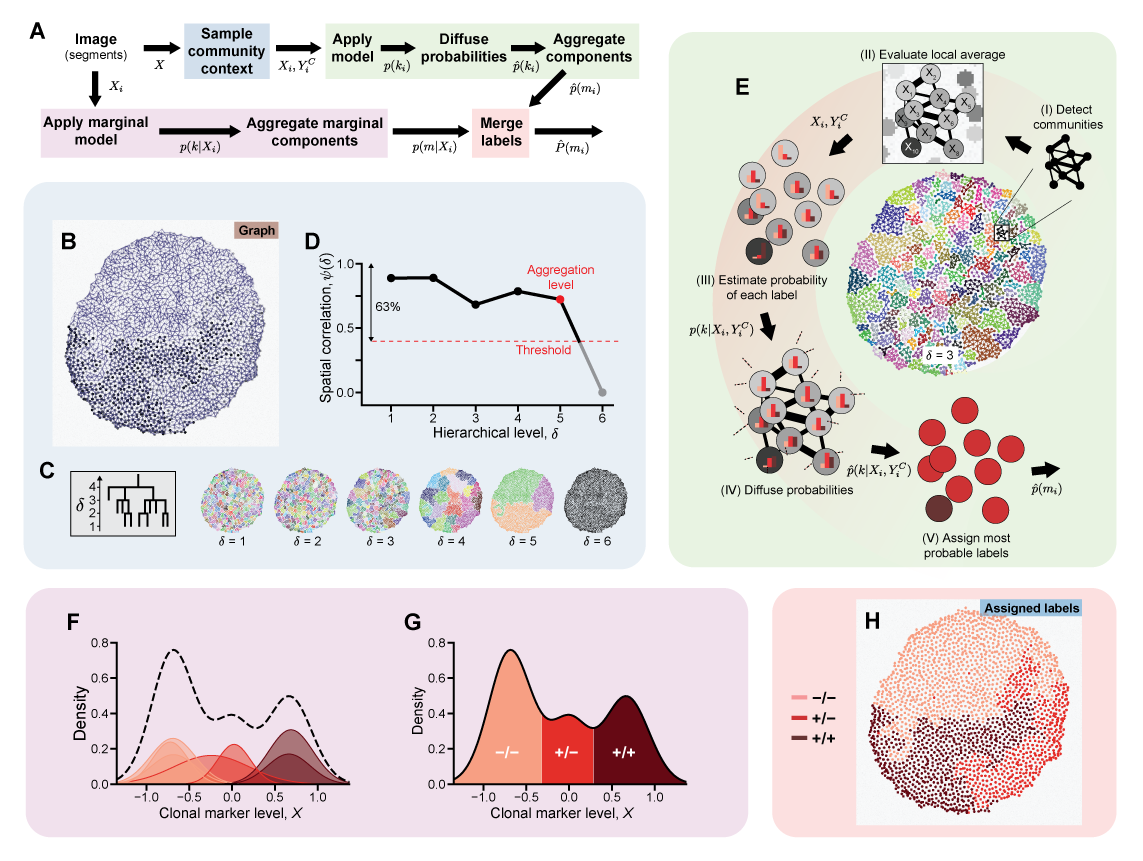
\includegraphics[scale=1.0]{./figure_S4}
\caption[Simple two-species competitive binding model]{\textbf{A simple two-species competitive binding model} (A) Model schematic. (B) Theoretical Pnt site occupancy as a function of transcription factor abundance. Equivalent binding affinities are used for illustrative purposes. Simultaneous proportional increases in absolute abundance of both species have minimal impact on Pnt occupancy, while varying ratio confers maximal change.}
\label{fig:ratio:figS4}
\end{figure}

However, the situation is more complex for Pnt and Yan. While there are several well-documented target genes that contain common binding sites for Pnt and Yan \cite{Halfon2000,Xu2000,Flores2000,BoisclairLachance2018}, Yan binds these enhancers with higher affinity than Pnt \cite{Xu2000}. Moreover, recent experiments suggest a scenario in which Pnt and Yan differentially interpret the structural syntax of \textit{cis}-regulatory modules \cite{BoisclairLachance2018}. This complex phenomenon is a consequence of cooperative recruitment between adjacent chromatin-bound Yan molecules. Yan monomers are able to polymerize via their sterile alpha motif (SAM) binding domains, enabling tightly-bound Yan monomers at strong ETS sites to stabilize the recruitment of additional Yan monomers to adjacent, weaker ETS sites or non-ETS sites \cite{Qiao2004,BoisclairLachance2018}. These cooperative effects could conceivably bias the competition between Pnt and Yan, which led us to consider a more complex model.

Hope, Rebay, and Reinitz recently introduced a modeling framework in order to probe the effects of \textit{cis}-regulatory syntax on Yan binding site occupancy \cite{Hope2017}. The model considers an ensemble of microstates, each defined by a unique configuration of vacant or Yan-bound sites. Each microstate is assigned a thermodynamic potential based on the cumulative influence of strong ETS-binding, weak non-ETS binding, and polymerization. We augmented this model by incorporating Pnt as a second transcription factor that competes for occupancy of the same binding sites (Fig. \ref{fig:ratio:figS5}A). 

Our formulation of the model is based on a single \textit{cis}-regulatory element consisting of $n$ adjacent binding sites, each of which may be designated as ETS or non-ETS. Each binding site may only exist in one of three binding states; bound by a single copy of Yan, bound by a single copy of Pnt, or unbound. Thermodynamic potentials are assigned to each binding state using two parameters for each transcription factor. The parameter $\alpha_X$ defines the free energy of transcription factor $X$ binding to an ETS site, while $\beta_X$ defines the free energy of binding to a non-ETS site (Fig. \ref{fig:ratio:figS5}A). A unique configuration of binding states for all $n$ binding sites constitutes a single microstate, $k$. The thermodynamic potential of each microstate is given by the superposition of thermodynamic potentials for each of its constituent binding sites. For each microstate, the stabilizing effect of polymerization is incorporated via a third parameter, $\gamma_X$, that defines the free energy of SAM-SAM binding between a pair of similar transcription factors bound to adjacent sites. The net result is a total thermodynamic potential, $\Delta G_k$, for each microstate. An example enumeration of all possible microstates for an element consisting of one ETS site preceding two non-ETS sites is provided in Figure \ref{fig:ratio:figS5}B. The statistical frequencies of each microstate are obtained via the canonical ensemble:
\begin{equation}
p_k = \frac{\displaystyle exp( \frac{-\Delta G_k}{RT} ) [P]^{a_P(k)}[Y]^{a_Y(k)} } {\displaystyle \sum_{k} {exp(\frac{-\Delta G_k}{RT})[P]^{a_P(k)}[Y]^{a_Y(k)}}}
\end{equation}
in which $p_k$ is the frequency of microstate $k$, $[P]$ and $[Y]$ are the Pnt and Yan concentrations, $a_P(k)$ and $a_Y(k)$ are functions representing the number of bound molecules of $P$ and $Y$ within microstate $k$, $T$ is a fixed temperature set to 300 K, and $R$ is the gas constant. Fractional occupancies for each binding site correspond to the cumulative frequency of all microstates in which the site is occupied by a given transcription factor. Overall fractional occupancies may then be computed by summing across all sites within the element.

\begin{figure}[h]
\centering
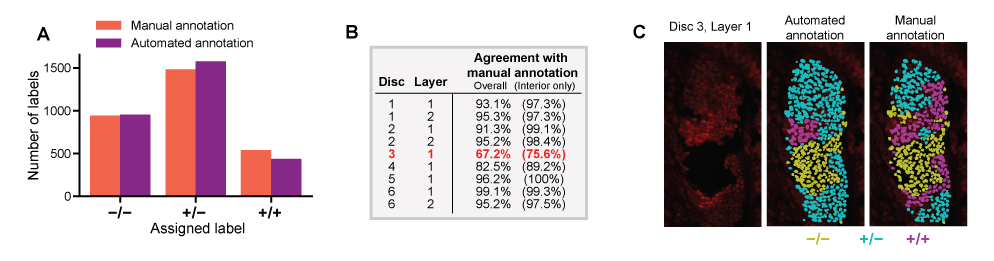
\includegraphics[width=0.9\columnwidth]{./figure_S5}
\caption[Thermodynamic model of transcription factor DNA binding.]{\textbf{Thermodynamic model of transcription factor DNA binding.} (A) Summary of thermodynamic interactions within one microstate of a cis-regulatory element containing one ETS site and two non-ETS sites. Solid black lines represent individual binding sites. Green and magenta rectangles denote Pnt and Yan molecules. Example thermodynamic potentials of strong ETS-binding, weak non-ETS binding, and polymerization interactions are denoted by $\alpha_{Pnt}$, $\beta_{Yan}$, and $\gamma_{Yan}$, respectively. For this microstate, $a_P(k)=1$ and $a_Y(k)=2$. (B) Enumeration of all possible microstates for a cis-regulatory element of length 3 in which only the first site carries the ETS designation. Solid black lines denote binding sites, green and magenta rectangles denote bound Pnt and Yan molecules. The cumulative thermodynamic potentials of each microstate, $\Delta G_k$, are listed beside each graphical depiction. Visual representation is adapted from \cite{Hope2017}. (C) Relative thermodynamic contributions of binding site affinity versus polymerization to microstate statistical frequencies as a function of Pnt and Yan concentration. For each point in the plane, influence of site affinity was calculated by weighting the sum of all ETS and non-ETS thermodynamic potentials for each microstate by the statistical frequency of the corresponding microstate. The influence of polymerization was analogously determined. The shown color scale reflects the relative magnitude of these two summations, normalized by limits of zero and complete polymerization.}
\label{fig:ratio:figS5}
\end{figure}

Using this model, we sought to characterize the sensitivity of Pnt binding site occupancy to changes in the Pnt-to-Yan ratio without neglecting cooperativity derived from \textit{cis}-regulatory syntax. We first considered a scenario in which Yan and Pnt did not exhibit cooperativity (Fig. \ref{fig:ratio:fig3}A). In the absence of stabilizing SAM-SAM interactions, the landscape of overall binding site occupancy is identical to that obtained with the simple binding model described above (Figs. \ref{fig:ratio:fig3}B and \ref{fig:ratio:figS4}B). Increasing the Pnt-to-Yan ratio revealed a gradual increase in Pnt occupancy for all individual binding sites (Fig. \ref{fig:ratio:fig3}C). This titration contour closely resembles a Langmuir isotherm or Michaelis-Menten saturation curve \cite{Fogler1987}.

We then introduced a stabilizing SAM-interaction for Yan (Fig. \ref{fig:ratio:fig3}D). The resultant landscape of overall Pnt binding site occupancy is clearly distinguished from the simple binding model by a sharpening of the transition from Yan to Pnt dominance in occupancy (Fig. \ref{fig:ratio:fig3}E). Weighting the energetic contributions of binding strength and polymerization by the statistical frequency of each microstate revealed that the transition is driven by an abrupt change in the dominant binding mechanism. Polymerization effects dominate binding site occupancy when the Pnt-to-Yan ratio is low, while binding strength dominates when the ratio is high (Fig. \ref{fig:ratio:figS5}C).

Increasing the Pnt-to-Yan ratio revealed nonlinear transitions from low to high Pnt occupancy for each individual binding site (Fig. \ref{fig:ratio:fig3}F). These transitions resemble Hill functional forms \cite{Fogler1987}, indicating the emergence of sharp thresholds that delimit distinct regimes of transcriptional output. At low Pnt-to-Yan ratios, Yan is able to polymerize and occupies all binding sites. At some critical Pnt-to-Yan ratio, Pnt-bound sites intersperse Yan-bound sites such that Yan is no longer able to polymerize. Pnt then out-competes Yan as the ratio increases further. These results recapitulate the long-standing notion that cooperative DNA-binding sensitizes transcriptional output to changes in transcription factor activity.

Assuming binding sites are saturated, then relative occupancy by Pnt and Yan is agnostic to changes in the absolute abundance of either factor, as long as the Pnt-to-Yan ratio remains constant. This mechanism, coupled with cooperativity, would enable modest changes in the Pnt-to-Yan ratio to elicit large changes in DNA binding site occupancy by either factor, and presumably large changes in mRNA synthesis given the opposing transcriptional effects of Yan and Pnt.

\begin{figure}[h!]
\centering
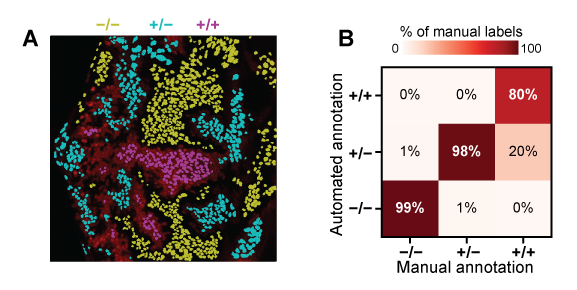
\includegraphics[width=1.0\columnwidth]{./figure_3}
\caption[Cooperative DNA-binding sensitizes promoters to the Pnt-to-Yan ratio.]{\textbf{Cooperative DNA-binding sensitizes transcriptional output to the Pnt-to-Yan ratio.} (A) Cartoon of competition between Pnt and Yan for occupancy of mutual binding sites in the absence of Yan polymerization. (B) Overall binding site occupancy as a function of transcription factor abundance in the absence of Yan polymerization. Color scale reflects overall Pnt site occupancy. A diverging scale was used because all sites are fully saturated at total transcription factor concentrations above 1 nM. Under the range of conditions shown, this implies that Yan occupies all sites left vacant by Pnt. Simultaneous proportional increases in absolute abundance of both species have minimal impact on Pnt occupancy (dashed arrow), while varying ratio confers gradual change (solid arrow). (C) Pnt occupancy of individual binding sites as a function of Pnt-to-Yan ratio in the absence of Yan polymerization. Contours correspond to a vertical path traversed across panel B at a fixed Yan concentration of 50 nM. All binding sites behave similarly. (D) Cartoon of competition between Pnt and Yan for occupancy of mutual binding sites when Yan polymerizes via its SAM domain. (E) Overall binding site occupancy as a function of transcription factor abundance when Yan polymerizes via its SAM domain. Color scale and arrows retain their meaning from panel B. (F) Pnt occupancy of individual binding sites as a function of Pnt-to-Yan ratio when Yan polymerizes via its SAM domain. Contours correspond to a vertical path traversed across panel E at a fixed Yan concentration of 50 nM. Line colors reflect binding site positions within the \textit{cis}-regulatory element. Sites at intermediate distances from the strong ETS site (green lines) transition at higher ratios than those nearest and furthest from the strong ETS site (blue and yellow lines).}
\label{fig:ratio:fig3}
\end{figure}

\section{Regulation stabilizes the ratio against varying Pnt and Yan concentrations}

Equilibrium modeling suggests cell state transitions can proceed normally amidst individual or cell-to-cell fluctuations in the absolute concentrations of Pnt and Yan. We tested this idea by varying the genetic dosage of the \textit{pnt} gene from one to two copies. Protein output in \textit{Drosophila} is approximately proportional to the number of copies of any given gene \cite{Lucchesi1973}, validating our strategy. We found that the eyes of adult flies were morphologically indistinguishable across this \textit{pnt} dosage range (Fig. \ref{fig:ratio:figS1}A,B). A similar lack of dosage sensitivity had been previously observed with the \textit{yan} gene \cite{Pelaez2015a}. Because both sets of genetic manipulations should in theory change the Pnt-to-Yan ratio, the absence of overt phenotypes suggested that either cell state transitions are not sensitive to this ratio or that there are active feedback mechanisms that drive cells back to the ideal ratio.

To distinguish between these possibilities we asked whether the ratio of Pnt-GFP to Yan protein is sensitive to the abundance of Pnt-GFP protein. We quantified Pnt-GFP levels in eye cells containing either one or two copies of the \textit{pnt-gfp} transgene in a \textit{pnt} mutant background. As expected, Pnt-GFP protein concentration varied proportionally to \textit{pnt-gfp} gene copy number (Fig. \ref{fig:ratio:fig4}A,B). Interestingly, average Yan protein concentration also scaled with \textit{pnt-gfp} gene copy number (Fig. \ref{fig:ratio:fig4}C,D) resulting in an essentially identical Pnt-to-Yan protein ratio (Fig. \ref{fig:ratio:fig4}E). The dependence of Yan protein output on \textit{pnt-gfp} gene copy number parallels our previous finding that \textit{pnt} mutant cells had lower Yan protein concentrations \cite{Pelaez2015a}. We conclude that the network regulating Yan protein output compensates for variation in the abundance of Pnt to maintain a constant Pnt-to-Yan ratio.

Effective control of the Pnt-to-Yan ratio would require a similar dependence of Pnt protein output on the concentration of Yan. We assessed this prediction by quantifying Pnt-GFP protein in cells with different copy numbers of the \textit{yan} gene. Due to the embryonic lethality of \textit{yan}-null mutations, we conducted this experiment by inducing \textit{yan}-null clones in the developing eye, and using an Ubi-mRFPnls marker to identify genotypes of cells in the clones. Cells with different \textit{yan} gene dosages exhibited different Pnt-GFP protein concentration (Figs. \ref{fig:ratio:fig4}F,G and \ref{fig:ratio:figS6}A,B). Notably, Pnt-GFP levels were correlated with \textit{yan} gene dosage in progenitor cells immediately posterior to the MF. We quantified this effect by measuring Pnt-GFP protein concentration in cells with or without a copy of the wildtype \textit{yan} gene (Figs. \ref{fig:ratio:fig4}H). Pnt-GFP expression was higher in cells with one or more copies of \textit{yan} than in cells with zero copies (Mann-Whitney \textit{U} test, $p<0.001$), suggesting that Pnt protein output is dependent on the abundance of Yan protein. Overall, these data suggest cells compensate for fluctuations in Pnt or Yan protein abundance by adjusting the level of the opposing protein. 

Yan expression was not quantified in this experiment due to limiting availability of fluorescence reporters with non-overlapping emission spectra. We were therefore unable to determine whether the Pnt-to-Yan ratio is robust to changes in \textit{yan} dosage. However, the data suggest that cells respond to an increase in \textit{yan} gene dosage by increasing their Pnt protein levels. Our wildtype data indicate that the Pnt-to-Yan ratio remains constant over time (Fig. \ref{fig:ratio:fig1}K). It is therefore possible that mutual compensation between Pnt and Yan help preserve the ratio by buffering fluctuations in the abundance of either protein. If this mutual compensation occurs on a sufficiently fast timescale, it could account for the constant Pnt-to-Yan ratio we observed in progenitor cells, despite large changes in Pnt and Yan concentration over time (Fig. \ref{fig:ratio:fig1}E,J).

\begin{figure}[p!]
\centering
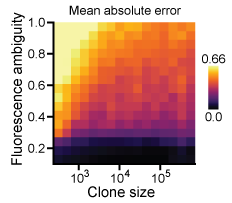
\includegraphics[width=0.9\columnwidth]{./figure_4}
\caption[P:Y ratio is stabilized against varying Pnt and Yan concentrations.]{\textbf{The Pnt-to-Yan ratio is stabilized against varying Pnt and Yan concentrations in progenitor cells.} (A-D) Moving averages of (A, B) Pnt-GFP and (C, D) Yan levels in progenitor and differentiating cells with one (A, C) versus two (B, D) copies of the \textit{pnt-gfp} gene. Measurements used DAPI to mark nuclei. Colors denote cell type. Shaded regions are bootstrapped 95\% confidence intervals for the moving average. (E) Comparison of Pnt-to-Yan ratios between progenitor cells with one versus two copies of \textit{pnt-gfp} during cell fate transitions. Colors denote cell fate transition periods for each R cell type. These time periods are defined in each disc by the times spanned by the first ten identifiable R cells. The concurrent progenitor cell populations are selected from these time windows. Light grey filled boxes denote 1x \textit{pnt-gfp}, dark grey filled boxes denote 2x \textit{pnt-gfp}. Pnt-to-Yan ratios in progenitor cells are indistinguishable between gene dosages during R8, R2/R5, and R1/R6 cell fate transitions (KS 2-sample test, $p<0.001$). (F-G) Confocal image slice of progenitor nuclei in a disc containing loss-of-function \textit{yan} clones. RFP fluorescence marks wildtype \textit{yan}. (H) Quantitative comparison of Pnt-GFP expression between \textit{yan} genotypes. Progenitor cells were assigned \textit{yan} genotypes based on measured RFP level, and Pnt-GFP levels were corrected to account for fluorescence bleed-through (see \ref{ch:clones:correction}). Pnt-GFP levels decrease when no gene copies of \textit{yan} are present (Mann-Whitney \textit{U} tests). Red dots denote the median of each distribution, thick grey lines denote the interquartile range.}
\label{fig:ratio:fig4}
\end{figure}

\section{Notch signaling lowers the Pnt-to-Yan ratio in progenitor cells}

Progenitor cells are dynamically stable about a constant Pnt-to-Yan ratio, but this fixed ratio changes as cells transition to an R cell state. We next asked how the ratio is set in individual cells targeted for differentiation. Notch and RTK signaling provide both transcriptional and post-transcriptional inputs to the Yan-Pnt network \cite{Graham2010}, and therefore present prime candidates to establish and modulate the Pnt-to-Yan ratio. The two pathways generally exert opposing influence on R cell state transitions. Notch signaling is required to maintain progenitor cells in a multipotent state \cite{Fortini1993}, and ensures proper patterning of the first group of R cells by constraining the proximity of adjacent R8 cells \cite{Lubensky2011,Gavish2016}. Conversely, RTK signaling is required to initiate each of the subsequent R cell state transitions \cite{Freeman1996}. Both signaling pathways influence the Pnt-Yan network in multipotent eye cells \cite{Brunner1994,Rebay1995,Rogge1995}. Notch stimulates Yan expression \cite{Rohrbaugh2002}, while RTK activates PntP2 and stimulates PntP1 expression \cite{Brunner1994,Shwartz2013} while attenuating the pulse of Yan expression \cite{Rebay1995,Pelaez2015a}. The precise influence of Notch and RTK signaling on the Pnt-to-Yan ratio are difficult to predict as the two pathways are coupled by feedback within and beyond the Pnt-Yan network \cite{Rohrbaugh2002,Kumar2003,Voas2004}.

We used a temperature-sensitive \textit{Notch} mutant \cite{Cagan1989} to measure the impact of Notch-mediated signaling on Pnt-GFP and Yan. We divided the eye field into two regions for analysis purposes (Fig. \ref{fig:ratio:figS7}A, dashed yellow line). The first region starts anterior to the MF and ends in the region of R8 cell specification. The second region extends $\sim$ 10 columns of R8 cells posterior to the first region. These regions contain the first and second pulses of Pnt-GFP, respectively (Fig. \ref{fig:ratio:figS7}A, thick black lines).

At the non-permissive temperature, progenitor cells had visibly reduced Yan levels (Fig. \ref{fig:ratio:figS7}A,B), consistent with previous reports of Yan expression's dependence on Notch signaling in the developing eye disc \cite{Rohrbaugh2002}. Pnt-GFP levels were also reduced in region 1, but appeared close to normal at later times (Fig. \ref{fig:ratio:figS7}A,B). Attempts to study ratio dynamics in mutant eye discs were challenging. Notch is essential for proper patterning of R8 cells, so the mutant eye discs had distorted spacing of R8 cells at the non-permissive temperature (Fig. \ref{fig:ratio:figS7}C). The irregularity of the intervals between adjacent columns of R8 cells precluded the conversion of spatial position along the anterior-posterior axis to developmental time. As an alternative to our standard quantitative analysis, we visualized the effects of Notch by mapping the pixel-wise difference between Pnt-GFP and Yan to a diverging color scale (Fig. \ref{fig:ratio:fig5}A,B). Direct visualization of the ratio yielded a very similar view of differential Pnt-GFP/Yan expression, but was prone to computational errors imparted by zero-valued pixels. This qualitative analysis was limited to optical sections specifically spanning the progenitor cells.

At the non-permissive temperature, the \textit{Notch} mutant showed a consistently higher Pnt-to-Yan ratio in progenitor cells in region 2 (Fig. \ref{fig:ratio:fig5}A). This observation suggests that Notch signaling maintains a low Pnt-to-Yan ratio in these undifferentiated cells. The known role of Notch in maintaining multipotency in region 2 \cite{Fortini1993} is consistent with our hypothesis that cell state transitions are mediated by the transcription factor ratio.

The Notch mutant revealed more complex behavior in region 1, where the first group of R cell transitions occur. In this region Notch is required for patterning of the R8 lattice \cite{Lubensky2011}. At the permissive temperature, there was a periodic pattern in the Pnt-to-Yan ratio of progenitor cells (Fig. \ref{fig:ratio:fig5}B). Clusters of cells with higher ratio alternated with clusters with lower ratio. We quantified the periodicity of this pattern by evaluating the similarity of ratios between cells as a function of their separation distance (Fig. \ref{fig:ratio:fig5}C). We detected periodic spatial patterns with a constant period of oscillation that was approximately equivalent to the length scale separating adjacent R8 cells (Fig. \ref{fig:ratio:fig5}D,E). Since young R8 cells have elevated Pnt-to-Yan ratios, we infer that periodic clusters of high-ratio progenitor cells give rise to the R8, R2/R5, and R3/R4 cells. At the non-permissive temperature, the Pnt-GFP/Yan pattern was strongly impaired (Fig. \ref{fig:ratio:fig5}B). The ratio was more uniform along the dorso-ventral axis, and while there were modestly detectable oscillations in the ratio, their period was not stable (Fig. \ref{fig:ratio:fig5}F,G).

These results are consistent with the consensus understanding that Notch signaling serves dual roles in R8 fate determination. Initially, Notch pushes clusters of progenitor cells towards an R8 cell state. Later, Notch restricts differentiation to ensure only one cell per cluster adopts an R8 state \cite{Baker1997,Li2001,Lubensky2011}. If Notch signaling is inhibited, very few high Pnt-to-Yan ratio clusters and R8 cells are formed because the first step is blocked \cite{Baker1997}. If cell state transitions are coupled to the Pnt-to-Yan ratio, then the \textit{Notch} mutant would not be expected to have high-ratio clusters in region 1. This is precisely what we observed.

\begin{figure}[h!]
\centering
\includegraphics[width=1.0\columnwidth]{./figure_5}
\caption[Notch signaling lowers the Pnt-to-Yan ratio in progenitor cells.]{ (Continued on the next page.) }
\label{fig:ratio:fig5}
\end{figure}
\begin{figure}[h!]
\contcaption{\textbf{Notch signaling lowers the Pnt-to-Yan ratio in progenitor cells.} (A) Visualization of relative Pnt and Yan expression in progenitor cells in region 2 when Notch signaling is active (left panel) and restricted (right panel). Color scale reflects the difference between Pnt-GFP and Yan fluorescence. Black lines denote periods of elevated Pnt-GFP expression. See methods for details on post-processing of images. (B) Visualization of relative Pnt and Yan expression in progenitor cells during the first wave of cell state transitions. Black arrow marks the morphogenetic furrow. Gold arrows annotate clusters of elevated ratio. (C-E) Quantification of spatial periodicity in the Pnt-to-Yan ratio among progenitor cells immediately posterior to the MF when Notch signaling is active. (C) Spatial correlation functions for progenitor cells in four eye discs. Black lines show the moving average pairwise correlation of Pnt-to-Yan ratios between cells as a function of their separation distance along the dorso-ventral axis. Oscillatory forms indicate alternating regions of similar and dissimilar behavior relative to the population-wide mean. Lines are obtained via first-order Savitzky-Golay filtration with a window size of 50. Shaded region shows a bootstrapped 95\% confidence interval for the moving average. Cell counts are annotated above each correlation function. Red lines are the expected outcome for random expression (no pattern). (D) Normalized Lomb-Scargle periodograms for each disc. Spectra are constructed from individual progenitor cell measurements for periods ranging 50 to 200 px. Grey lines denote spectral power attributed to each oscillation period. Dashed red significance thresholds are obtained by bootstrap resampling the ratio intensities. Asterisks denote signal frequencies exceeding the confidence threshold. In all discs, a pattern in Pnt-to-Yan ratios repeats on a length scale of 73-82 px when Notch signaling is active. (E) Distribution of dorso-ventral separation distances between adjacent R8 neurons within a single column of ommatidia within each disc. Mean values are comparable to the detected oscillation periods. (F,G) No periodicity is detected above the significance threshold when Notch signaling is restricted.}
\end{figure}

\section{Ras signaling elevates the Pnt-to-Yan ratio in progenitor cells}

RTK signals received by progenitor cells trigger their transition to R cell states \cite{Freeman1996}. We quantitatively probed the effect of RTK signaling on Pnt-GFP dynamics and the Pnt-to-Yan ratio by using a temperature-sensitive $EGFR^{ts}$ allele that restricts RTK signaling \cite{Kumar1998}. At high temperatures, the mutant blocks RTK signal transduction, which triggers cell death and allows only R8 neuron patterning. However, animals raised at intermediate temperatures achieve normal recruitment of R8, R2/R5, and R3/R4 neurons, but fail to recruit most R1/R6 and R7 cells \cite{Pelaez2015a}.

At intermediate temperatures, the entire second pulse of Pnt-GFP expression disappeared upon restriction of EGFR activity (Fig. \ref{fig:ratio:figS8}A). Because the second pulse can be predominantly ascribed to PntP2 expression (Fig. \ref{fig:ratio:fig1}I), this result conflicts with a report that PntP2 expression is not dependent upon RTK signaling \cite{Shwartz2013}. At intermediate signaling, Yan levels were also reduced, resulting in Pnt-to-Yan ratios that were indistinguishable from wildtype during the second wave of state transitions (Fig. \ref{fig:ratio:figS8}B,C).

\begin{figure}[h]
\centering
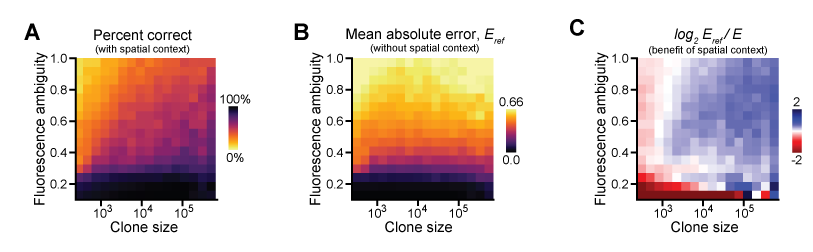
\includegraphics[width=1.0\columnwidth]{./figure_S8}
\caption[Pnt and Yan expression dynamics in $EGFR^{ts}$ eye discs.]{\textbf{Pnt and Yan expression dynamics in $EGFR^{ts}$ eye discs.} (A-C) Effects of $EGFR^{ts}$ on (A) Pnt-GFP, (B) Yan, and (C) Pnt-to-Yan ratio dynamics in progenitor cells. Lines are moving averages across 250 sequential cells. Shaded regions are bootstrapped 95\% confidence intervals for the mean. Solid lines and grey shading denote wildtype controls. Dashed lines and red shading denote restricted EGFR signaling. Black bars denote second period of elevated Pnt-GFP expression.}
\label{fig:ratio:figS8}
\end{figure}

We next asked whether RTK signaling is sufficient to induce an increase in the Pnt-to-Yan ratio of progenitor cells by expressing a constitutively-active form of Ras \cite{Simon1991,Fortini1992}. This construct uses a \textit{sev} promoter to drive Ras expression, limiting its effects to the second region of Pnt-GFP expression. Constitutive Ras activity dramatically increased the amplitude and duration of the second pulse of Pnt-GFP expression in progenitor cells (Fig. \ref{fig:ratio:fig6}A) but did not significantly alter Yan expression dynamics (Fig. \ref{fig:ratio:fig6}B). This yielded a sustained increase in Pnt-to-Yan ratio in progenitors during the second wave of state transitions (Fig. \ref{fig:ratio:fig6}C), as well as the ectopic differentiation of R cells. As previously reported \cite{Fortini1992}, supernumerary cells included extra R7 cells, as well as additional R cells whose identities were not discerned due to their aberrant positioning.

We sought to determine whether these ectopic R cells emerged from a pool of progenitors with abnormally high Pnt-to-Yan ratios. Focusing our analysis on progenitor cells concurrent with the ectopic induction of R cells revealed that their ratios were higher than those of wildtype progenitor cells at comparable times (Fig. \ref{fig:ratio:fig6}D,E grey boxes). Nearly all young supernumerary R cells had ratios that were within the range of mutant progenitor cells, and were above the range observed in wildtype cells (Fig. \ref{fig:ratio:fig6}D,E blue and purple markers). These observations suggest that abnormally high Pnt-to-Yan ratios in progenitor cells accompany ectopic R cell state transitions.

\begin{figure}[h!]
\centering
\includegraphics[scale=1.0]{./figure_6}
\caption[Ras signaling elevates the Pnt-to-Yan ratio in progenitor cells.]{\textbf{Ras signaling elevates the Pnt-to-Yan ratio in progenitor cells.} (A-C) Effects of constitutive Ras signaling on (A) Pnt-GFP, (B) Yan, and (C) Pnt-to-Yan ratio dynamics in progenitor cells. Lines are moving averages across 250 sequential cells. Shaded regions are bootstrapped 95\% confidence intervals for the mean. Solid lines and grey shading denote wildtype controls. Dashed lines and red shading denote constitutive Ras signaling by $Sev>Ras^{V12}$. Black bars denote periods of elevated Pnt-GFP expression. We previously reported a modest increase in the duration of Yan-YFP expression in $Sev>Ras^{V12}$. mutant progenitor cells \cite{Pelaez2015a}, but this difference was not detected using the Yan antibody. (D, E) Comparison of Pnt-to-Yan ratios between wildtype and $Sev>Ras^{V12}$ progenitor cells concurrent with the ectopic differentiation of (D) unidentified R cells and (E) R7 cells in $Sev>Ras^{V12}$ discs. Markers denote the first 25 supernumerary R cells.}
\label{fig:ratio:fig6}
\end{figure}

\section{Ratiometric control as a model for cell fate commitment}

Successful cell state transitions usually require changes in mRNA and protein expression, which are often dictated by transcription factors. It is widely believed that expression depends on the absolute concentration of these factors \cite{Spitz2012}. We have identified a scenario in which cells respond to the ratio in abundance of two transcription factors rather than to the absolute concentration of either protein. This novel mechanism is made possible by several characteristics of the system. First, target genes of these factors are induced when cells transit to differentiated states, and expression of these targets is necessary for differentiation \cite{Xu2000,Nagaraj2002}. Second, both factors bind to the same DNA sites in their target genes. Third, they exert opposing effects on transcription.

A theoretical analysis reveals that, under these conditions, relative site occupancy by either factor determines whether or not a target gene is transcribed. When binding sites are saturated, the probability a site is occupied by one of the factors is controlled by the ratio of factor concentrations and not by the absolute concentration of the factors. This mechanism allows the transcription factors to have pulsatile expression dynamics and still consistently regulate transcription. Regulation of genes through pulsatile dynamics of competing transcription factors with opposing effects has been reported in yeast \cite{Lin2015}. In the developing eye, however, this competition relies on the ratio of the two factors to differentially regulate genes. Perhaps the pulsatile dynamics of Pnt and Yan allow R cell state transitions to be restricted to a specific period of developmental time.

We developed a model to demonstrate that stabilizing interactions between adjacently bound monomers can sensitize enhancer occupancy to the relative abundance of two competing transcription factors. The model does not offer a rigorous characterization of the competition between Pnt and Yan for a specific enhancer, as the data required to construct such a model are not available. For example, it is unknown whether nuclear concentrations of Pnt and Yan protein are of an equivalent order of magnitude in differentiating eye cells. Similarly, we do not know the strength, number, or arrangement of bindings sites in the enhancers targeted by Pnt and Yan. However, the conclusions we have drawn from our model do not rely upon specific values for these variables, and are consequently not anchored to the specific details of any one system. 

In general, the proposed ratiometric sensing mechanism is well suited when either or both transcription factors bind their target sites in a manner stabilized by cooperative interactions. Like its human ortholog TEL1 \cite{Kim2001}, DNA-bound Yan monomers enhance recruitment of Yan to adjacent binding sites through stabilizing SAM-SAM polymerization \cite{Zhang2010}. We show theoretically that such cooperativity could generate threshold-like behavior and cause ultrasensitive switching in site occupancy between Yan and Pnt. In this model, the switching is agnostic to the absolute abundance of either transcription factor as long as their relative ratio can be precisely controlled. This mechanism would enable state transitions to proceed despite variation in protein concentrations driven by fluctuations in metabolism, cell volume, expression noise, environmental conditions, genetic polymorphisms, or gene copy number.

The average Pnt-to-Yan ratio is dynamically stable about an approximately constant value within each cellular state, and only exhibits transient fluctuations when cells switch states. These dynamics reflect the capacity of the system to coordinate the relative expression of the two transcription factors. We have found that the abundance of each transcription factor depends upon the expression of the other factor. Dependencies of this type are often depicted as positive or negative regulation in cartoons of qualitative regulatory interactions (Fig. \ref{fig:ratio:fig7}A). We believe that as biology becomes increasingly quantitative it will be more fruitful to emphasize an empirical description of system dynamics based on control theory (Fig. \ref{fig:ratio:fig7}B).

From a control perspective, a system of cellular components monitors the relative abundance of Pnt and Yan and takes corrective action when the ratio deviates from a specified reference value. The particular components responsible for implementing control may remain unspecified. This perspective eschews molecular events in favor of minimizing complexity, but preserves the salient features of a detailed molecular mechanism and can enable quantitative predictions.

Fluctuations in the absolute abundance of one factor are mitigated by compensatory adjustment of the other. Notch or RTK activity could modulate Pnt or Yan protein levels to transiently perturb the Pnt-to-Yan ratio (Fig. \ref{fig:ratio:fig7}B, dashed black arrow). These signals could permanently set the ratio by adjusting the reference value (Fig. \ref{fig:ratio:fig7}B, dashed red arrow). We advocate this control theoretic perspective because it more accurately conveys the fundamental strategy underlying system behavior. Furthermore, accurate model predictions would only require the evaluation of a small number of parameters that characterize Pnt-to-Yan ratio dynamics, obviating the need for experimental measurement of reaction rates during R cell specification in \textit{Drosophila}.

\begin{figure}[h!]
\centering
\includegraphics[scale=1.0]{./figure_7}
\caption[Conceptual models for regulation of the Pnt-to-Yan ratio.]{\textbf{Conceptual models for regulation of the Pnt-to-Yan ratio.} (A) Cartoon of qualitative regulatory interactions suggests Pnt and Yan protein levels are coupled by reciprocal positive feedback (solid lines), while Notch and Ras signaling adjust the Pnt-to-Yan ratio by modulating the levels of each protein (dashed lines). (B) Block diagram of ratio control in the Pnt-Yan network. Lines represent values, rectangles indicate functions, and the circle is a comparison point. The Pnt-to-Yan ratio is compared against a basal reference value, and the difference is fed into a regulatory network that acts to drive the ratio back toward the reference value. Extracellular signals transiently perturb the ratio by modulating Pnt or Yan protein levels (dashed black line), or set the ratio by adjusting the reference value (dashed red line).}
\label{fig:ratio:fig7}
\end{figure}

We have shown that dynamic changes in the Pnt-to-Yan ratio are coupled to cell state. Our favored interpretation is that the ratio determines which state a cell is in. Direct testing of this hypothesis remains difficult because the observed ratio control strategy precludes gene-level manipulation of the ratio. Instead, we acknowledge that our observations are correlative. We cannot discard the possibility that Notch and RTK signaling regulate state transitions in a manner that is not only mediated by the Pnt-to-Yan ratio but by other mechanisms as well. We emphasize, however, that ratio control enforces stability when cells are in one state, which implicates the ratio as an active cell state determinant. Moreover, qualitatively different approaches to experimentally manipulate the ratio affected cell state transitions in a consistent manner. Both Notch inhibition and Ras activation increase the ratio and cause abnormal R cell state transitions \cite{Fortini1992,Yang2006}. Single-cell dynamical measurements of Yan and specific Pnt isoforms during isoform-specific perturbations may ultimately prove necessary to determine definitively whether ratios directly mediate transitions. The regulatory mechanism described here provides insight into how the relative dynamics of competing transcription factors can be used to pattern complex epithelia, and may also aid design of synthetic regulatory systems based on ratiometric sensing.

\graphicspath{ {figures/metabolism/} }

% CONTRIBUTIONS
%%%%%%%%%%%%%%%%%%%%%%%%%%%%%%%%%%%

\chapter{Layered repression synchronizes development with cellular metabolism}
\label{ch:metabolism}

A manuscript resembling this chapter was coauthored with Justin Cassidy, Rachael Bakker, Ritika Giri, Nicol\'{a}s Pel\'{a}ez, Bryan Eder, Anna Bobrowska, Neda Bagheri, Lu\'{i}s Amaral, and Richard Carthew. The preprint is available at \url{https://doi.org/10.1101/548032}. All of the experiments were conceived, designed, and executed by my colleagues. In particular, Justin Cassidy obtained the wealth of data that ultimately made this work possible. My contributions include all of the computational modeling and simulations. Much of the text was either written by or under the guidance of Professor Richard Carthew.

% MANUSCRIPT
%%%%%%%%%%%%%%%%%%%%%%%%%%%%%%%%%%%% 

\section{Background on the environmental dependence of developmental tempo}

Animal development occurs over a defined timescale, which requires control of the rates of developmental processes. Developmental timescales are an intrinsic feature of a species, and are not necessarily determined by external clocks \cite{Ebisuya2018}. Rather, the pace of development is encoded in the genome. Development occurs via a stereotypic sequence of events involving cell division, growth, movement, apoptosis, polarization, and differentiation. Correct assembly of functional structures depends upon synchronization of cell division and differentiation events \cite{Foe1989,Sulston1983}. Small variation in timing produces variation in structure that is observed between individuals \cite{Francesconi2014,Poullet2016}. Abnormal timing can result in structural defects that lead to compromised survival \cite{Moss2007}.

While developmental tempo is a fundamental property of a species, it can vary under different conditions. For example, temperature affects the pace of development in many ectotherms, such as arthropods, nematodes, fish, and reptiles \cite{Atlas1935,Davidson1944,Kuntz2014,Zuo2011}. Diet and food intake also affect organismal growth rate and the pace of development for many species, including humans \cite{Arendt1997,Brown2004,Metcalfe2001,Pontzer2016}. Finally, cellular metabolism can alter the pace of development. For example, the evolutionarily conserved \textit{Clk1} gene encodes a mitochondrial enzyme necessary for normal cellular respiration \cite{Felkai1999}, and loss of the \textit{clk1} gene in nematodes and mice results in developmental delays \cite{Levavasseur2001,Nakai2001,Wong1995}. In \textit{Drosophila}, restricting glucose consumption by cells slows development \cite{Brogiolo2001,Layalle2008,Rulifson2002,Shingleton2005}. West and colleagues formulated a general quantitative model that relates developmental tempo to both cellular metabolic rate and temperature \cite{Gillooly2002}. Strikingly, the model fits meta-data spanning several kingdoms, suggesting a universal relationship between metabolism and developmental tempo.

Many developmental processes involve specification of different cell types in a stereotyped sequence. All of these differentiated cell types originate from progenitor cells. The sequence of cell differentiation is driven by changes in the gene expression program within progenitors. Gene regulators, typically transcription factors, are sequentially activated and repressed, resulting in transient periods of increased activity. During these periods, they change gene expression in the progenitors. This coincides with and causes a temporal series of cell fate decisions. Since these regulators frequently interact with one another, the entire cascade constitutes a gene regulatory network (GRN). Such GRNs have been characterized for embryogenesis \cite{Cusanovich2018,Lawrence1992}, development of the central nervous system \cite{Kohwi2013}, and development of the sensory nervous system \cite{Cepko2014}. Because the tempo of development can vary, GRN dynamics must be able to reliably adjust to a variable timing mechanism. Therefore, understanding how these GRNs adapt to a variable timescale is crucial for understanding the mechanisms of animal development.

Phenomenological observations suggest that there are limits to the timescales to which development may adapt. While broiler chickens have been successfully bred for rapid growth, frequent abnormalities in musculoskeletal development are evident in such breeds \cite{Julian2005,Whitehead2003}. Animals (and humans) experience hyper-normal growth rates if they initially experience delayed growth \cite{Arendt1997}. Such compensatory growth is linked to a variety of developmental and physiological defects \cite{Metcalfe2001}. Conversely, slowing growth can alleviate defects caused by mutations that impair development. As first noted by T.H. Morgan, morphological phenotypes can be suppressed by limiting the nutrition of mutant animals \cite{Child1939,Morgan1915,Morgan1929,Sang1963}. Likewise, raising animals under lowered temperatures can sometimes suppress the phenotypes of mutations that are not classical \textit{ts} alleles \cite{Child1935,Krafka1920,Lewis1980,Villee1943}. Collectively, these observations suggest an unknown mechanism ensures successful developmental outcomes amidst variability in developmental tempo.

Here, we have explored this mechanism. We find that impairing gene repression in GRNs causes developmental errors but only when cell metabolism and growth rate are normal. When either energy metabolism or protein anabolism are reduced, developmental errors are reduced or even suppressed. We find that this relationship between metabolism and repression is so prevalent that the entire microRNA family becomes unnecessary when metabolism is slowed. Using a general quantitative modeling framework for regulated gene expression, we show that multiple layers of weak repression render gene expression dynamics independent of variable biochemical rates. When rates are modestly reduced, fewer repressors are needed to ensure normal expression dynamics. We experimentally validate this model prediction by following GRN dynamics in \textit{Drosophila}. Our findings support a new mechanism whereby layers of gene repression allow development to occur over a wider range of time scales, enabling development to proceed faster if metabolic conditions allow for it. The need for flexible error frequency suppression could provide an evolutionary impetus for the high prevalence of genetic redundancy.

\section{Repressors are less impactful when metabolism is reduced}

Developmental patterns arise from directed dynamics of cell-cell signaling and gene regulation. The sensory organs of \textit{Drosophila} are a classic system with which to study these phenomena \cite{Quan2005}. A broad collection of gene mutations has specific effects on the formation of various sensory organs, and these mutations have been instrumental in uncovering the molecular mechanisms of sensory organ development. The affected genes encode transcription factors, microRNAs, signaling factors, and other gene regulators. We used such gene mutations to readdress the relationship between reduced metabolism and phenotype suppression that was first observed by Morgan \cite{Morgan1915,Morgan1929}. We did so by scoring \textit{Drosophila} sensory mutant phenotypes under conditions of reduced energy metabolism. We generated animals that had reduced metabolism by genetic ablation of their insulin producing cells (IPCs) in the brain (Fig. \ref{fig:metabolism:fig1a}A). This ablation reduces the amount of glucose that cells consume \cite{Rulifson2002}, resulting in 70\% slower development (Fig. \ref{fig:metabolism:fig1a}B), and small but normally proportioned adults (Fig. \ref{fig:metabolism:fig1a}C) \cite{Rulifson2002}.

\begin{figure}[h!]
\centering
\includegraphics[scale=1.0]{./figure_1a}
\caption[IPC ablation slows development by restricting energy metabolism.]{\textbf{IPC ablation slows development by restricting energy metabolism.} (A) Strategy to ablate IPCs (red) in the young fly brain. Gal4 expressed under control of the promoter for the \textit{Insulin-Like Peptide 2} (\textit{ILP2}) gene drives production of the pro-apoptotic protein Reaper (Rpr) specifically in IPCs of the brain. (B) The number of days after egg laying (AEL) at which the first individual in either wildtype or $ILP2>Rpr$ populations eclosed (hatched from pupa into adult) is shown, as is the time at which the last individual in each population eclosed. Population sizes for wildtype and $ILP2>Rpr$ were 126 and 185, respectively. (C) Adult body size is affected by IPC ablation. Two females that were raised at the same time and temperature. The left $yw$ animal has normal metabolism, whereas the right animal has slowed metabolism due to ablation of its IPCs.}
\label{fig:metabolism:fig1a}
\end{figure}

We first examined mutations affecting formation of the compound eye. The microRNA miR-7 represses expression of the Yan transcription factor in the developing eye \cite{Li2005}. Yan protein is transiently expressed in the eye \cite{Pelaez2015a}, and is cleared from differentiating photoreceptor (R) cells by multiple repressors acting on its transcription, mRNA stability, and protein stability \cite{Graham2010}. When the \textit{miR-7} gene was specifically ablated in the compound eye of an otherwise wildtype animal, it resulted in small malformed adult eyes due to errors in R cell differentiation (Fig. \ref{fig:metabolism:fig1b}A). This phenotype was highly penetrant in genetically mosaic animals (Fig. \ref{fig:metabolism:fig1b}B). However, when energy metabolism was slowed by IPC ablation, loss of \textit{miR-7} was much less important for the formation of correctly patterned eyes (Fig. \ref{fig:metabolism:fig1b}B). We also examined mutations affecting cell-cell signaling. The Sevenless (Sev) receptor tyrosine kinase hyper-activates MAP kinase in certain eye progenitor cells, leading to enhanced turnover of the Yan protein \cite{Rebay1995}. This enables cells to differentiate into R7 photoreceptors \cite{Voas2004}. When \textit{sev} is mutated, cells completely fail to differentiate as R7 photoreceptors. This effect was readily apparent by staining for an R7-specific marker protein (Fig. \ref{fig:metabolism:fig1b}C). However, slowing metabolism allowed a small but significant number of \textit{sev} mutant cells to become R7 photoreceptors (Fig. \ref{fig:metabolism:fig1b}D). Importantly, since the \textit{sev} mutant makes no protein products \cite{Banerjee1987}, rescue of the mutant phenotype was not simply due to more functional Sev protein molecules being present in slowly metabolizing cells.

\begin{figure}[h!]
\centering
\includegraphics[scale=1.0]{./figure_1b}
\caption[Eye developmental defects are rescued by slower energy metabolism.]{\textbf{Eye developmental defects are rescued by slower energy metabolism.} (A) Genetically mosaic individuals with a $miR\hyphy 7^+$ body and a $miR\hyphy  7$ mutant eye. Left individual with mispatterned eye has its IPCs intact while the right individual with a normally patterned eye has had its IPCs ablated by $ILP2>Rpr$. (B) Eye patterning is more normal if mosaic individuals slowly metabolize due to IPC ablation. Sample population sizes were between 264 and 467 individuals. P values from Chi-square test with Yates correction. (C) Eye cells stained for specific protein markers such that R7 cells (white) can be distinguished from other R cells (purple) and bristle cells (green). Each ring-like cluster of R cells is an ommatidium. Null mutation of \textit{sev} results in no R7 cells (right). (D) Slow metabolism due to IPC ablation increases the fraction of ommatidia that contain an R7 cell in \textit{sev} mutants. Each data point represents one eye sample; between 481 and 837 ommatidia were scored for R7 cells within each eye sample. P value is from a one-way ANOVA with Bonferroni correction.}
\label{fig:metabolism:fig1b}
\end{figure}

We also examined formation of other sensory organs for evidence of metabolic interactions. Large sensory bristles develop in a highly stereotypic pattern over the \textit{Drosophila} body. The protein Senseless (Sens) transiently appears in a cluster of proneural cells before one cell is chosen to differentiate into a sensory bristle \cite{JafarNejad2003}. MicroRNA miR-9a represses Sens protein expression, and \textit{miR-9a} mutants frequently develop ectopic sensory bristles because this repression is missing (Fig. \ref{fig:metabolism:fig2}A,B) \cite{Cassidy2013,Li2006}. However, when \textit{miR-9a} mutants had their IPCs ablated, errors in bristle number were greatly reduced (Fig. \ref{fig:metabolism:fig2}C).

The protein Hairy directly represses transcription of the proneural genes \textit{achaete} and \textit{scute} during selection of cells for bristle fates \cite{VanDoren1994}. Mutation of \textit{hairy} causes some individuals to develop ectopic large bristles. However, this effect of \textit{hairy} mutation was strongly suppressed when energy metabolism was slowed (Fig. \ref{fig:metabolism:fig2}C). We saw a similar effect on a \textit{cis}-regulatory module (CRM) that represses gene transcription. The \textit{Sternopleural} (\textit{Sp-1}) mutation is present in a CRM located on the 3' side of the \textit{wingless} (\textit{wg}) gene \cite{Neumann1996a}, causing Wg misexpression and development of ectopic bristles \cite{Neumann1996a}. However, the ectopic bristle phenotype of the $wg^{Sp-1}$ mutant was completely reversed under conditions of slowed energy metabolism (Fig. \ref{fig:metabolism:fig2}D).

\begin{figure}[h!]
\centering
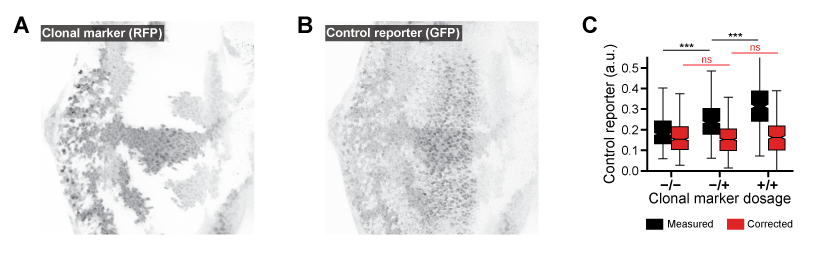
\includegraphics[scale=1.0]{./figure_2}
\caption[Reducing energy metabolism rescues sensory bristle patterning.]{\textbf{Sensory bristle developmental defects are rescued by slower energy metabolism.} (A) Number of scutellar bristles is frequently greater than four in a \textit{miR-9a} mutant whereas it is almost invariably four in wildtype. (B) Distribution of scutellar bristle numbers in wildtype and $miR\hyphy  9a$ mutant populations. Population sizes for wildtype and $miR\hyphy  9a$ were 301 and 222, respectively. The cumulative frequency distributions between wildtype and mutant were significantly different ($p<0.0001$, KS test). (C) IPC ablation increases the proportion of $miR\hyphy  9a$ mutants and \textit{hairy} mutants that have the wildtype number of scutellar bristles. ****, $p<0.0001$; n.s., $p>0.05$ (D) Under normal metabolic conditions, $wg^{Sp-1}$ displays an increased number of sternopleural bristles. IPC ablation dramatically increases the number of mutant individuals with the wildtype number of three sternopleural bristles. Shown in each panel is the number of individuals with bristle number of three versus the total number of individuals scored. IPC ablation significant suppresses the $wg^{Sp-1}$ mutant phenotype ($p<0.0001$, Fishers exact test).}
\label{fig:metabolism:fig2}
\end{figure}

\section{MicroRNAs are dispensable when metabolism is reduced}

The mutations thus far examined affect diverse types of regulators, including microRNAs, transcription factors, and signaling molecules. Despite this diversity, all of the mutations have something in common: they affect repressive interactions between genes. To explore the prevalence of this relationship between gene repression and metabolism, we eliminated an entire family of regulatory repressors that control all stages of \textit{Drosophila} development. The microRNA family is composed of 466 distinct microRNAs in \textit{Drosophila melanogaster} \cite{Kozomara2014}. Virtually all microRNAs require Dicer-1 (Dcr-1) protein for their proper biosynthesis, and Ago1 protein as a partner to repress target gene expression \cite{Carthew2009a}. Protein-null mutations in either \textit{dcr-1} or \textit{ago1} genes are lethal \cite{Pressman2012}. We raised different null \textit{dcr-1} mutants under conditions of slower energy metabolism, and found that many more animals survived development (Fig. \ref{fig:metabolism:fig3}A). \textit{Ago1} null mutants are normally 100\% embryonic lethal, but mutant lethality was broadly suppressed when animals slowly metabolize due to IPC ablation (Fig. \ref{fig:metabolism:fig3}B). The mutants survived to adulthood, and most survivors had normal eye and bristle patterns as well as other body structures, indicating the rescue of a massive array of developmental defects (Fig. \ref{fig:metabolism:fig3}C). Rescue could also be seen when Ago1 was specifically ablated in cells of the compound eye; eye development was strongly rescued by slower energy metabolism (Fig. \ref{fig:metabolism:fig3}D). Therefore, a major class of regulatory repressors is rendered non-essential when energy metabolism is slowed.

\begin{figure}[h!]
\centering
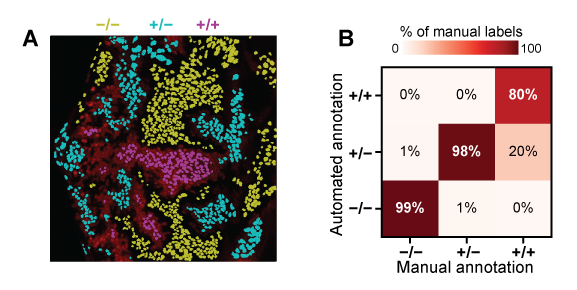
\includegraphics[scale=1.0]{./figure_3}
\caption[All microRNAs are dispensable when energy metabolism is slowed.]{\textbf{The microRNA family is dispensable when energy metabolism is slowed.} (A) The pupal viability of various \textit{dcr-1} nonsense mutants is fully rescued when IPCs are ablated in the mutants. (B) Adult viability of various \textit{ago1} missense and nonsense mutants is rescued when IPCs are ablated in the mutants. (C) Representative \textit{ago1} adults with normal or slowed metabolism. (D) Genetically mosaic individuals with $ago1^+$ bodies and $ago1^{W894X}$ mutant eyes. Left, representative individual with normal metabolism has almost no eye tissue (24/24 animals had this phenotype). Right, representative individual with slowed metabolism has rescued eye tissue. Of 70 such animals analyzed, 46 had this phenotype, 20 had normal eyes, and 4 had eyes that resembled the left animal. This is a statistically significant difference ($p<0.0001$; Chi square with Yates correction). Error bars, s.d. ****, $p<0.0001$; **, $p<0.01$; *, $p<0.05$; n.s., $p>0.05$}
\label{fig:metabolism:fig3}
\end{figure}

\section{Modeling the emergence of developmental errors in variable environments}

We turned to computational modeling in order to elucidate the biochemical mechanism linking gene repression, developmental phenotypes, and metabolism. Because this relationship appeared relevant to many GRNs during many stages of \textit{Drosophila} development, we sought to directly model the emergent properties of these systems rather than the specific regulatory mechanisms behind them. We therefore explored the mechanism using a general modeling framework premised on the progressive restriction of cell potential over time. Each step of restriction corresponds to a change in gene expression; gene products are synthesized, act, and then are eliminated until they are again needed in other cells (Fig. \ref{fig:metabolism:fig4a}A). Temporally localized expression allows signaling molecules and transcription factors to be repeatedly used to build different body structures at different times. On the other hand, transient expression dynamics require GRN components to remain synchronized with the processes they govern. If they fall out of rhythm, developmental errors occur. We therefore modeled the transient expression and regulation of a single gene within an intracellular cascade of developmental gene expression (Fig. \ref{fig:metabolism:fig4a}A, red line).

\begin{figure}[h!]
\centering
\includegraphics[scale=1.0]{./figure_4a}
\caption[A dynamic model of gene regulation during cell fate determination.]{\textbf{A dynamic model of gene regulation during cell fate determination.} (A) A program of gene expression occurs as a single cell passes through a series of developmental states. The model focuses on transient expression of a single gene within a cascade of gene expression. A state change is defined as the induction of gene expression by upstream gene products (input) and the action of the gene product (output). (B) Schematic representation of the response to a transient input, which can be either an extracellular or intracellular signal. Gene expression output is subject to layers of negative regulation acting at the gene, transcript, and protein levels. (C) Control representation of a single feedback loop as depicted in B. Boxes contain transfer functions, open circles indicate summation points, and closed circles indicate exclusive switches for each repressor. (D) Protein expression may be subject to layers multiple repressors acting in parallel.}
\label{fig:metabolism:fig4a}
\end{figure}

\subsection{Mathematical model of gene expression}
\label{metabolism:model:linear}

To model the dynamics of gene expression, we defined a linear time invariant system that describes the time evolution of activated DNA (\textit{D}), mRNA (\textit{R}), and protein (\textit{P}) in response to an inductive stimulus (\textit{I}). These state variables describe the extent of gene expression at any point in time. Transitions between each of the variables' discrete states are governed by the set of psuedo-elementary reactions listed in Table \ref{metabolism:model:rxns}.

% TABLE OF REACTIONS
%%%%%%%%%%%%%%%%%%%%
\begin{table}[h!]
\centering
\footnotesize
\caption[Elementary steps of gene expression]{\textbf{Elementary steps of gene expression}}
\label{metabolism:model:rxns}
\begin{tabular}{L{1.75in} C{1.1in} C{0.75in} C{1.35in}}
\toprule
\bfseries Reaction & \bfseries Transition & \bfseries Propensity & \bfseries Param. [min\textsuperscript{-1}] \\
\midrule
Gene activation & $\Delta D \to \Delta D + 1$ & $k_1 \Delta I$ & 1 \\
Transcription & $\Delta R \to \Delta R + 1$ & $k_2 \Delta D$ & 1 \\
Translation & $\Delta P \to \Delta P + 1$ & $k_3 \Delta R$ & 1 \\
Gene deactivation & $\Delta D \to \Delta D - 1$ & $\gamma_1 \Delta D$ & 1 \\
Transcript decay & $\Delta R \to \Delta R - 1$ & $\gamma_2 \Delta R$ & 10\textsuperscript{-2} \\
Protein decay & $\Delta P \to \Delta P - 1$ & $\gamma_3 \Delta P$ & 10\textsuperscript{-3} \\
\bottomrule
\end{tabular}
\end{table}

GRNs use layers of negative regulation to attenuate expression of target genes (Fig. \ref{fig:metabolism:fig4a}B). In our model, a system of regulatory components monitors the relative abundance of a target protein that dictates a cell fate transition. When the abundance of this protein increases, the regulatory components sense the increase in protein levels and act to down-regulate it, either at the level of gene transcription, mRNA stability, or protein stability (Fig. \ref{fig:metabolism:fig4a}C). The particular mechanisms responsible for implementing regulation may remain unspecified. Instead, we abstract all modes of regulation using the independent and linear elementary reactions listed in Table \ref{metabolism:model:regulation}. Multiple repressors often act in parallel to attenuate the expression of target genes. These control elements can be thought of as independent repressors working in parallel to bring the protein level back to a basal steady-state (Fig. \ref{fig:metabolism:fig4a}D). 

% TABLE OF REGULATION
%%%%%%%%%%%%%%%%%%%%%
\begin{table}[h!]
\centering
\footnotesize
\caption[Elementary steps of gene regulation]{\textbf{Elementary steps of gene regulation}}
\label{metabolism:model:regulation}
\begin{tabular}{L{1.75in} C{1.1in} C{0.75in} C{1.35in}}
\toprule
\bfseries Reaction & \bfseries Transition & \bfseries Propensity & \bfseries Param. [min\textsuperscript{-1}] \\
\midrule
Transcriptional feedback & $\Delta D \to \Delta D - 1$ & $\eta_1 \Delta P$ & \num{5.0e-4} \\
Feedback on mRNA & $\Delta R \to \Delta R - 1$ & $\eta_2 \Delta P$ & \num{1.0e-4} \\
Feedback on protein & $\Delta P \to \Delta P - 1$ & $\eta_3 \Delta P$ & \num{5.0e-4} \\
\bottomrule
\end{tabular}
\end{table}

In the continuum limit, this model yields a deterministic system of ordinary first-order differential equations:
\begin{equation}
\label{metabolism:model:ode}
\begin{aligned}
\frac{dD}{dt}&=k_1I-\gamma_1D - \sum\limits_{}^{N} \eta_{1}P \\
\frac{dR}{dt}&=k_2D-\gamma_2R - \sum\limits_{}^{N} \eta_{2}P \\
\frac{dP}{dt}&=k_3R-\gamma_3P - \sum\limits_{}^{N} \eta_{3}P \\
\end{aligned}
\end{equation}
where $k_i$ are activation, transcription, or translation rate constants, $\gamma_i$ are degradation constants, $\eta_i$ are feedback strengths, and each species may be subject to $N$ independent repressors. Equation \ref{metabolism:model:ode} describes the time evolution of transcription rates, transcript abundance, and protein abundance. When these targets are induced by exogenous stimuli, their timely attenuation ensures that protein expression remains transient. The resultant dynamics resemble a simple pulse response. Our model therefore eschews molecular detail while preserving the salient features of gene expression dynamics that are relevant to developmental outcomes. This coarse-grained modeling strategy emphasizes an empirical view of GRN dynamics, and facilitates quantitative predictions at the organismal scale.

The model was not designed to capture the specific details of the various GRNs probed by our experiments. Instead, it provides a platform to survey the general principles that govern the dynamics of developmental processes. Namely, we developed a model that allowed us to ask how protein expression dynamics change when repressors are removed. In each of our model systems, protein expression is transient. Beginning at a basal steady state, expression is driven by upstream components of the developmental program. The ensuing expression dynamics can therefore be considered a response to perturbation.

\subsection{Model relation to control theory}

Control theory provides a theoretical foundation underpinning the response of systems displaced from steady state. One of its core principles is the notion of local stability; that is, systems deviate linearly about a fixed point. Models based on this principle seek to describe how system output deviates from its steady state value in time. Describing our model with control terminology, protein level remains fixed about a basal steady state. Deviations from the basal level are driven by a transient disturbance. The disturbance induces activation of a gene, which induces transcription of mRNAs, which proceed to induce translation of protein. These three state variables are linearized about their steady state values:
\begin{equation}
\label{metabolism:model:deviations}
\begin{aligned}
\Delta D &= D - \lim_{t \to \infty} D(t) \\
\Delta R &= R - \lim_{t \to \infty} R(t) \\
\Delta P &= P - \lim_{t \to \infty} P(t) \\
\end{aligned}
\end{equation}
where the prefix $\Delta$ signifies a deviation variable and the limit denotes the steady state concentration for a fixed level of the input signal.

Protein levels relax back to steady state as the stimulus subsides. Control theory offers further insight when the relaxation process is mediated by one or more regulatory actors. In each of the experimentally surveyed GRNs, regulatory species such as microRNAs detected an increase in protein levels and acted to attenuate protein expression. These actors implement feedback control; they sense deviations in system output and exert an opposing response to drive the system back toward steady state. Neglecting their precise mechanisms of action, we can capture the influence of these \emph{controllers} on system output with a single parameter, the feedback strength $\eta_i$ for controller $i$. For simplicity we assume these regulatory mechanisms provide \emph{proportional control}, meaning they modulate the deviations defined by Equation \ref{metabolism:model:deviations} with a strength proportional to the output protein level. This \emph{proportional only} scheme is incapable of input tracking and could not reject a sustained disturbance \cite{Yi2000}. However, proportional only control provides an adequate representation of system dynamics because our model depicts an intermediate step in a cascade of developmental processes whose inputs and outputs are inherently localized in space and time (Fig. \ref{fig:metabolism:fig4a}A).

When expressed in the Laplace frequency domain (see \cite{Seborg2011}), the system is readily described by three sequential first-order transfer functions:
\begin{equation}
\begin{aligned}
\Delta D(s) &= \Big( \frac{\frac{k_1}{\gamma_1}}{\frac{1}{\gamma_1}s+1} \Big) \Big [\Delta I(s) - \sum\limits_{}^{N} \frac{\eta_{1}}{k_1}\Delta P(s) \Big ] \\
\Delta R(s) &= \Big( \frac{\frac{k_2}{\gamma_2}}{\frac{1}{\gamma_2}s+1} \Big) \Big [\Delta D(s) - \sum\limits_{}^{N} \frac{\eta_{2}}{k_2}\Delta P(s) \Big ] \\
\Delta P(s) &= \Big( \frac{\frac{k_3}{\gamma_3}}{\frac{1}{\gamma_3}s+1} \Big) \Big [\Delta P(s) - \sum\limits_{}^{N} \frac{\eta_{3}}{k_3}\Delta P(s) \Big ] \\
\end{aligned}
\end{equation}
where the argument $s$ is the complex frequency. Given this formulation, control theory provides a wealth of insight into the stability and dynamic character of pulsatile protein expression when the feedback strengths are varied. The transfer functions propagate deviations in the stimulus level (the input) to deviations in protein level (the output). A signal block diagram representation reveals that each regulatory process listed in Table \ref{metabolism:model:regulation} confers closed-loop control of protein levels following their induction (Fig. \ref{fig:metabolism:figS1a}). The internal dynamics of this system dictate its sensitivity to perturbation. Restated symbolically, the magnitude and duration of protein expression are governed by the relative influence of the process and controller gains, $K_{Pi} = k_i/\gamma_i$  and $K_{Ci} = \eta_i/k_i$. The contributions of each regulatory element $\eta_i$ are additive, and may therefore be combined into a single controller gain for each point of actuation $i$. This formulation allows us to emulate the loss of a repressor simply by lowering the relevant controller gain.

\begin{figure}[h!]
\centering
\includegraphics[scale=1.0]{./figure_S1a}
\caption[Block diagram depiction of the mathematical model.]{\textbf{Block diagram depiction of the mathematical model.} Boxes contain transfer functions relating upstream and downstream variables, open circles indicate summation points. Transfer functions are expressed in the Laplace frequency domain.}
\label{fig:metabolism:figS1a}
\end{figure}

\subsection{Simulation of developmental errors due to repressor loss}
\label{metabolism:model}

Protein expression follows a biphasic trajectory after reception of a transient stimulus (Fig. \ref{fig:metabolism:fig4b}A,B, left panel). If there were no noise or variability, the protein level would be deterministic over time. However, protein dynamics vary because gene expression is noisy \cite{Arias2006}, something that can be captured in the model simulations by incorporating intrinsic noise.

We then devised a scheme to relate protein expression dynamics to the likelihood of a successful developmental outcome. We define success as the ability of a GRN to attenuate protein expression in a timely manner, thus keeping pace with parallel components of the developmental program by triggering subsequent developmental events. We quantified errors in developmental outcome by defining a threshold that the output protein level must cross before a subsequent event can be triggered. Protein levels exceeding the threshold constitute errors in developmental outcome (Fig. \ref{fig:metabolism:fig4b}B, right panel). Notably, such errors become more frequent when one repressor is removed (Fig. \ref{fig:metabolism:fig4b}C). This property is observed over a broad range of parameter values, regardless of the manner in which repressors act, or the value at which the threshold is established (see Section \ref{metabolism:robust}).

The modeling framework allowed us to ask whether multiple layers of repression are less important for developmental outcome when energy metabolism is reduced. To answer this question, we halved the rate parameters of each ATP-utilizing reaction to reflect conditions of reduced energy metabolism (see Section \ref{metabolism:methods:conditions}). Although ATP content remains fairly constant in cells facing limited respiration, the fluxes of ATP synthesis and turnover are affected, manifesting in altered ratios of ATP to ADP and free phosphate \cite{Brown1992}. Anabolic processes such as protein synthesis are highly dependent on the ATP/ADP ratio \cite{Atkinson1977}. When we halved ATP-dependent rate parameters and compared model results from full versus partial repression, we observed that error frequency in developmental outcome did not increase when a repressor was lost (Fig. \ref{fig:metabolism:fig4b}D). This insensitivity to loss of a repressor persisted whether repression was transcriptional, post-transcriptional, or post-translational. The effect was observed across a wide range of model parameter values, irrespective of where the threshold was set, and regardless of whether a basal stimulus was present (see Section \ref{metabolism:robust}). In many cases the effect remained modestly apparent when the stimulus duration was extended to maintain comparable protein levels under conditions of reduced energy metabolism. In general, our modeling framework suggests that the frequency of developmental errors is less sensitive to changes in repression when energy metabolism is reduced.

\begin{figure}[h!]
\centering
\includegraphics[scale=1.0]{./figure_4b}
\caption[Simulated errors are less frequent when metabolism is reduced.]{\textbf{Simulated developmental errors are less frequent when metabolism is reduced.} (A-C) Simulated emergence of developmental errors. (A) A transient input signal drives (B) pulsatile protein expression dynamics. Simulations may be performed with two post-translational repressors in place (full repression), or with only one repressor in place (partial repression). Shaded regions correspond to the 98\% confidence band of simulated protein trajectories. We define the commitment time as the time needed for 99\% of simulations with full repression to cross a predefined threshold. With partial repression, the protein levels take longer to decay, so fewer simulations cross the threshold within the defined commitment time. We interpret each failure of a simulated protein level to decay below the threshold in time as a developmental error. (C) Error frequency is greater with partial repression. (D) The model suggests that errors will occur more frequently under partial repression regardless of how repressors act on gene expression (left panel). However, partial repression imparts fewer developmental errors when ATP-dependent parameter values are reduced by 50\% (right panel).}
\label{fig:metabolism:fig4b}
\end{figure}

Reduced glucose consumption by cells might not only limit ATP fluxes, but also hinder the synthesis of nucleotide and amino acid precursors required for RNA and protein synthesis. To simulate this scenario, we specifically reduced the rate parameters for RNA and protein production. Constraining these synthesis rates also suppressed the rise in error frequency when a repressor was lost (Fig. \ref{fig:metabolism:figS2b}).

\begin{figure}[h!]
\centering
\includegraphics[scale=1.0]{./figure_S2b}
\caption[Reduced biosynthesis diminishes the frequency of developmental errors.]{\textbf{Partial repression imparts few developmental errors when biosynthesis is reduced.} Construction is equivalent to the right panel of Figure \ref{fig:metabolism:fig4b}D. However, rather than fully reduced energy metabolism, only the RNA and protein synthesis rate parameter values were reduced by 50\%.}
\label{fig:metabolism:figS2b}
\end{figure}

Overall, our modeling framework is fully consistent with our experimental observations that multiple layers of repression cease to be important for developmental success under conditions of reduced carbon and energy metabolism. Furthermore, the modeling framework suggests that the phenotype suppression phenomenon may be driven by differences in protein expression dynamics that are dependent on metabolic conditions.

\section{Protein expression dynamics after partial repressor loss}

We quantified the extent to which the expression dynamics underlying developmental events were affected in our model. We first constructed a 98\% confidence band around the set of trajectories simulated with the full complement of repressors (see Section \ref{metabolism:methods:overexpression}). This confidence band provides lower and upper bounds for the expected protein level. We then evaluated the fraction of trajectories, $E(t)$, simulated with one repressor missing that fell above or below the confidence band at each point in time. Averaging these values across the time course yields a single metric that reflects the extent to which protein dynamics are affected by the loss of a repressor:
\begin{equation}
\text{Protein overexpression} \equiv \frac{1}{\tau}\int_{0}^{\tau}{E(t)}dt
\end{equation}
We evaluated this metric for a scenario in which an auxiliary post-transcriptional repressor, akin to a microRNA, is lost. Using typical metabolic parameters, 78\% of trajectories simulated without the post-transcriptional repressor exceed the confidence band generated under full repression (Fig. \ref{fig:metabolism:fig5}A). This overexpression effect is highly robust to parameter variation in the model (see Section \ref{metabolism:robust}). When ATP-dependent parameters were halved, only 16\% of trajectories exceeded the confidence band (Fig. \ref{fig:metabolism:fig5}B). The strong diminishment of overexpression under low metabolic conditions was also robust to extensive parameter variation. These results led us to predict that protein expression dynamics would be much less sensitive to repressor loss if we reduced metabolic rate.

We experimentally tested these predictions by measuring the expression dynamics of a key developmental regulatory protein, Yan. As shown in Chapter \ref{ch:ratio}, Yan exhibits pulsatile dynamics in the larval eye disc, where its expression is induced by a morphogenetic furrow that traverses the eye disc. Eye disc cells located in the morphogenetic furrow rapidly upregulate Yan protein abundance, as quantified by a YFP-tagged version \cite{Pelaez2015a}. Yan levels then gradually decay back to initial conditions within these cells, thus exhibiting pulsatile dynamics. We compared Yan-YFP dynamics in eye disc cells from normally metabolizing larvae and larvae with ablated IPCs (Fig. \ref{fig:metabolism:fig5}C,D). The same pulsatile dynamics were observed in both, but the amplitude of the pulse was slightly reduced and the duration was extended when metabolism was slower. Similar trends were predicted \textit{in silico} (Fig. \ref{fig:metabolism:fig5}A,B).

\begin{figure}[h!]
\centering
\includegraphics[scale=1.0]{./figure_5}
\caption[Expression dynamics are less affected when metabolism is reduced.]{\textbf{Expression dynamics are resistant to repressor loss when energy metabolism is reduced.} (A,B) Simulated expression of target protein output when it is under control of an auxiliary post-transcriptional repressor (green) or not under control of the repressor (orange). All simulations (green and orange) are also under control of a constitutive repressor. Shown are ten randomly-chosen samples from a total population of 5000 trajectories for each condition. (A) Simulations performed with normal ATP-dependent reaction rates. (B) Simulations performed following a 50\% reduction in the rate of ATP-dependent reactions. (C,D) Yan-YFP protein dynamics in eye disc progenitor cells. Time 0 marks the time at which Yan-YFP induction occurs. Solid lines are moving line averages. Shaded regions denote 95\% confidence intervals. Each line average is calculated from a composite of measurements of between 4,379 and 6,716 cells. (C) Yan-YFP dynamics for wildtype $Yan\hyphy YFP$ and mutant $Yan^{\Delta miR\hyphy  7}\hyphy YFP$ eyes under normal metabolic conditions. (D) Yan-YFP dynamics for wildtype and mutant genes when the IPCs have been ablated.}
\label{fig:metabolism:fig5}
\end{figure}

In the eye disc, Yan expression is repressed by the microRNA miR-7 \cite{Li2005}. There are four binding sites for miR-7 in the 3'UTR of \textit{yan} mRNA, and their mutation causes de-repression of Yan output. We eliminated miR-7 repression of \textit{Yan-YFP} by mutating the four binding sites in the 3'UTR of \textit{Yan-YFP} mRNA to make $Yan^{\Delta miR\hyphy  7}\hyphy YFP$. In normally metabolizing eye discs, Yan-YFP protein made from the mutated gene pulsed with greater amplitude and showed impaired decay when compared to Yan-YFP made from the wildtype gene (Fig. \ref{fig:metabolism:fig5}C). These dynamics recapitulate the effect of repressor loss predicted by our model (Fig. \ref{fig:metabolism:fig5}A). In contrast, Yan-YFP made from the mutated gene showed similar dynamics to protein made from the wildtype gene when metabolism was slowed (Fig. \ref{fig:metabolism:fig5}D). This behavior clearly resembled the simulated dynamics under conditions of reduced energy metabolism (Fig. \ref{fig:metabolism:fig5}B).

These measurements demonstrate that miR-7 has little to no impact on Yan expression dynamics when metabolism is slowed, and are consistent with the observed suppression of developmental errors when the same repressor is lost in the eye. The breadth of our model predictions further suggests that these effects are generalizable to other genes and repressors.

\section{Effect of full repression loss}

Our modeling framework is consistent with the hypothesis that multiple weak repressors allow GRN dynamics to faithfully couple to variable energy metabolism, with fewer repressors required when metabolic conditions are reduced. We then asked whether repression is needed at all under such conditions. We studied a model with a full complement of negative control elements and compared the results to a scenario in which all control elements were removed (Fig. \ref{fig:metabolism:fig6}A). Error frequencies approached 100\% under normal growth conditions. While expression dynamics were visibly less affected by repressor loss when ATP-dependent parameters were reduced, the error frequency remained very high (Fig. \ref{fig:metabolism:fig6}B). These results suggest that there are limits to the severity of perturbations for which reductions in energy metabolism can compensate, and reducing energy metabolism does not eliminate the need for gene repression altogether.

To test this prediction, we expressed in the eye a \textit{yan} mutant transgene that is insensitive to all known repression of \textit{yan} transcription, mRNA stability and protein stability \cite{Rebay1995}. The $Yan^{ACT}$ mutant adults had severely disrupted compound eye patterning (Fig. \ref{fig:metabolism:fig6}C). This mutant eye phenotype was not suppressed by ablation of the animals' IPC cells. Wildtype \textit{yan} transgenic adults with normal eye patterning were also unaffected by IPC ablation (Fig. \ref{fig:metabolism:fig6}D).

\begin{figure}[h!]
\centering
\includegraphics[scale=1.0]{./figure_6}
\caption[Reduced metabolism cannot compensate for complete loss of repression.]{\textbf{Reduced energy metabolism cannot compensate for complete loss of repression.} (A,B) Simulated expression of protein output both with (purple) and without (grey) any repression of the target gene. Shown are ten randomly chosen samples from a total population of 5000 trajectories for each condition. Error frequencies exceed 99\% irrespective of metabolic conditions. (A) Simulations performed under normal conditions. (B) Simulations performed following a 50\% reduction in the rate of ATP-dependent reactions. (C) Loss of eye tissue in a $yan^{ACT}$ mutant is not suppressed by slower metabolism. Representative individuals were taken from $N>100$ individuals for each condition. (D) Eye patterning in a $yan^{WT}$ control is not affected by slower metabolism. Representative individuals were taken from $N>100$ individuals for each condition.}
\label{fig:metabolism:fig6}
\end{figure}

\section{Limiting protein synthesis reduces the need for repressors}

The coupling of developmental dynamics to time can be explored with other aspects of metabolism. In particular, protein synthesis is an important determinant of rates of growth and development \cite{Lempiainen2009}. We used our modeling framework to investigate the impact of a twofold reduction in overall protein synthesis rate on GRN dynamics. The model suggests that expression dynamics are less affected and fewer developmental errors are incurred by loss of a repressor when protein synthesis rates are reduced (Fig. \ref{fig:metabolism:fig7a}). We again found this effect is robust to a wide range of parameter values and model assumptions (see Section \ref{metabolism:robust}).

\begin{figure}[h!]
\centering
\includegraphics[scale=1.0]{./figure_7a}
\caption[Simulated errors are less frequent when protein synthesis is reduced.]{\textbf{Simulated developmental errors are less frequent when protein synthesis is reduced.} The model predicts increased frequency of error with partial repression regardless of how auxiliary repressors act on gene expression (left panel is copied from \ref{fig:metabolism:fig4b}D). However, partial repression induces fewer errors when protein synthesis-dependent parameter values are reduced by 50\% (right panel).}
\label{fig:metabolism:fig7a}
\end{figure}

We tested this model prediction by genetically reducing the abundance of cytoribosomes in all cells in \textit{Drosophila}. We made use of loss-of-function mutations in genes encoding various ribosomal proteins (RPs), which cause the ``Minute'' syndrome of dominant, haploinsufficient phenotypes, including slower growth and development \cite{Marygold2007,Sæbøelarssen1998}. Heterozygous \textit{RP} mutants reduce the number of ribosomes per cell by approximately 50\%, and a total of 64 \textit{RP} genes exhibit a Minute syndrome when mutated. We selected a subset of these genes to reduce ribosome number.

We combined heterozygous \textit{RP} mutants with the repressor mutations we had previously studied. In all cases, the \textit{RP} mutants suppressed the developmental phenotypes of mutations in \textit{wg}, \textit{miR-7}, \textit{sev}, \textit{hairy}, and \textit{miR-9a} (Fig. \ref{fig:metabolism:fig7b}). This error frequency suppression was precisely the result predicted by our modeling.

\begin{figure}[h!]
\centering
\includegraphics[scale=1.0]{./figure_7b}
\caption[Reducing ribosome number rescues sensory organ development.]{\textbf{Reducing ribosome number rescues sensory organ development when repressors are lost.} (A) Loss of $miR\hyphy  7$ does not cause adult eye mispatterning when \textit{RpS3} is heterozygous mutant. (B) \textit{sev} mutants have more R7-positive ommatidia when either \textit{RpS3} or \textit{RpS13} are heterozygous mutant. Each datapoint represents one eye sample, and between 481 and 837 ommatidia were scored for R7 cells within each eye sample. (C) $wg^{Sp1}$ heterozygous individuals that are also heterozygous mutant for different \textit{RpS} genes have sternopleural bristle numbers more similar to wildtype. (D) Developmental accuracy is recovered for both $miR\hyphy 9a$ and \textit{hairy} mutants that are also heterozygous mutant for \textit{RpS13}. For all panels in B-E, error bars, s.d. ****, $p<0.0001$; ***, $p<0.001$; n.s., $p>0.05$.}
\label{fig:metabolism:fig7b}
\end{figure}

We also tested whether expression dynamics are affected by repressor loss under limiting translation conditions. The Sens protein is transiently expressed in proneural cells during selection of sensory bristle fates in the imaginal wing disc \cite{Nolo2000}. Bordering the presumptive wing margin, stripes of proneural cells express Sens protein over a spectrum of levels, reflecting heterogeneity in Wg and Notch regulation of its expression \cite{JafarNejad2006,Quan2005}. Moreover, miR-9a weakly represses \textit{sens} expression in these cells \cite{Li2006}. We recombineered a 19 kb \textit{sens} transgene, amino-terminally tagged with superfold GFP (sfGFP), that functionally replaced the endogenous \textit{sens} gene \cite{Cassidy2013,Venken2006}. Quantitative measurement of sfGFP fluorescence in individual proneural cells yielded the expected distribution of \textit{sens} expression (Fig. \ref{fig:metabolism:fig7c}A). We compared this distribution to one derived from individuals expressing a mutated sfGFP-\textit{sens} transgene in which its miR-9a binding sites had been mutated \cite{Cassidy2013}. Mutation of the miR-9a binding sites in \textit{sfGFP-sens} shifted the fluorescence distribution, and resulted in an average 1.45-fold increase in sfGFP-Sens levels (Fig. \ref{fig:metabolism:fig7c}B). We then tested the effects of miR-9a on \textit{sfGFP-sens} expression when the \textit{RpS13} gene was heterozygous mutant. Strikingly, loss of miR-9a regulation had less effect on sfGFP-Sens protein levels when ribosome numbers were reduced (Fig. \ref{fig:metabolism:fig7c}B). This behavior clearly resembled the effect predicted by the modeling framework.

\begin{figure}[h!]
\centering
\includegraphics[scale=1.0]{./figure_7c}
\caption[Reducing ribosome number diminishes \textit{sfGFP-sens} overexpression.]{\textbf{Reducing ribosome number diminishes \textit{sfGFP-sens} overexpression when miR-9a repression is lost.} (A) Frequency distribution of sfGFP-Sens protein level in cells bordering the wing margin of white prepupal wing discs. Shown are distributions of cells expressing either wildtype \textit{sfGFP-sens} or \textit{sfGFP-sens} in which miR-9a binding sites have been mutated. Each group represents \textgreater{} 15,000 cells. (B) \textit{sfGFP-sens} overexpression caused by miR-9a binding site mutations in \textit{RpS13} wildtype (green) and heterozygous mutant backgrounds (violet). Left panel shows median fold-change. Right panel shows the shift in the fluorescence distribution of sfGFP-Sens-positive cells as determined by a Mann-Whitney-Wilcoxon test. Error bars denote 95\% confidence intervals. Overexpression is attenuated in the \textit{RpS13} heterozygous mutant background.}
\label{fig:metabolism:fig7c}
\end{figure}

\section{Implications for the evolution of GRNs}

Growth and development are fueled by metabolism. This means that the tempo of development depends on metabolic rate. Thus, the dynamics of developmental gene expression must faithfully adjust to a variable time scale. We have shown that multi-layered weak repression within GRNs plays an unexpected function in synchronizing gene expression dynamics with the variable pace of the developmental program. Multiple repressors are required for accelerated development when metabolism is high, and they become functionally redundant when metabolism is low. Multiple repressors therefore allow for reliable development across a broader range of metabolic conditions than would otherwise be tolerated.

Our model explains long-standing observations linking nutrient limitation to suppression of mutant phenotypes \cite{Morgan1915,Morgan1929}. Presumably, such mutations cripple regulatory genes acting on developmental GRNs. Our model might also offer an explanation as to why animals that undergo above-normal growth exhibit compromised development \cite{Arendt1997,Metcalfe2001}. Wildtype GRNs might function across a limited range of metabolism, with functionality breaking down when metabolism exceeds that range.

Our varied analyses suggest that this relationship between metabolism and repression is ubiquitous. We found that the entire family of 466 microRNAs in \textit{Drosophila melanogaster} can become functionally dispensable when energy metabolism is slowed. The extensive literature on microRNA function in \textit{Drosophila} implicates them in practically all facets of the fruit fly's life \cite{Bushati2007,Carthew2017}. Various explanations have been provided for why this family of weak repressors has flourished in the animal kingdom, chief among them the idea that they act as buffers for gene expression \cite{Ebert2012}. We now posit that microRNAs also provide broad and flexible coupling of many developmental processes to variable timescales resulting from fluctuations in metabolism.

There is an alternative mechanism to explain phenotype suppression by reduced metabolism. This mechanism relies on a steady-state and not dynamical perspective of gene expression. Genome-wide gene expression patterns could conceivably change with organismal growth rate. This is the case for chemostat-grown yeast cells, where the expression of 27\% of all genes correlates with growth rate \cite{Brauer2008}. Most genes associated with stress response are overexpressed when cells grow at a slow rate \cite{Brauer2008,Lu2009}. Such differential gene expression could globally modulate dynamical processes such as protein folding and turnover, among others, and thereby attenuate phenotypes of genetic mutations. Abundance of molecular chaperones has been found to affect the penetrance of diverse gene mutations in \textit{C. elegans} and \textit{Drosophila} \cite{Casanueva2012,Rutherford1998}. However, these global effects do not explain why gene expression dynamics are conditionally dependent upon mutations in regulatory genes. We found that repression of Yan and Sens dynamics by microRNAs become more redundant when metabolic rates are slowed.

Metabolic rate increases exponentially with temperature as described by the Arrhenius equation \cite{Zuo2011}, resulting in an indirect temperature dependence of developmental tempo \cite{Gillooly2002}. Temperature also directly affects the rates of reactions within developmental GRNs \cite{Zuo2011}, yet developmental outcomes are generally robust to fluctuations in temperature across a limited range. Various molecular mechanisms have been invoked to explain this robustness. These include chaperones that create large protein-folding reservoirs \cite{Jarosz2010,Rutherford1998}, and regulatory circuits within interaction networks \cite{Li2009b}. Our model suggests a complementary mechanism for developmental robustness against temperature variation. By coupling gene expression dynamics with metabolism, weak repressors might neutralize the metabolic effects of temperature on developmental tempo. Indeed, loss of miR-9a regulation is less impactful on sensory organ development if the growth temperature is lowered \cite{Cassidy2013}. Likewise, raising animals under lowered temperatures can suppress the phenotypes of mutations that are not classical \textit{ts} alleles \cite{Child1935,Krafka1920,Lewis1980,Villee1943}.

Metabolic conditions drive variation about the intrinsic developmental tempo of each species. We have shown that layered weak repression within GRNs enables these fluctuations to occur without causing developmental errors. Metabolic conditions change in both space and time. Perhaps the selective advantage of a reliable developmental outcome amidst variable environmental conditions is a driving force in the evolution of gene regulatory networks.

\section{Robustness of modeling results}
\label{metabolism:robust}

We conducted numerous parameter sweeps to confirm the robustness of each result presented in this chapter. In each sweep, all model parameters were varied across a ten-fold range ($\pm \sim$three-fold). To efficiently sample the parameter space, we quasi-randomly sampled 2500 parameter sets from the multi-dimensional hyperspace defined by one order of magnitude variation in each of the model parameters. For each parameter set we independently ran six sets of five thousand simulations: 
\begin{enumerate}
	\item Full feedback with normal metabolism and translation
	\item Partial feedback with normal metabolism and translation
	\item Full feedback with reduced energy metabolism
	\item Partial feedback with reduced energy metabolism
	\item Full feedback with reduced protein synthesis	
	\item Partial feedback with reduced protein synthesis
\end{enumerate}
Full-repression systems were assigned two copies of each feedback element present in the corresponding partial-repression system. Error frequencies were evaluated as described previously. In total, this procedure constitutes one parameter sweep. 

Our parameter sweeps sampled an N-dimensional space, prompting us to seek a lower dimensional representation in order to visualize and discern any characteristic trends. One option is to project the results of all simulations onto each of the $N(N-1)/2$ orthogonal 2-D planes. Figure \ref{fig:metabolism:figS1b}A demonstrates this approach for error frequencies simulated with partial feedback and normal metabolism. While it clearly shows that error frequency is greater than 1\% for most combinations of parameter values (lots of dark spots), we find that the complexity of the 2-D visualization offers little additional insight. Instead, for all remaining parameter sweeps we opt for the simpler one dimensional projection of parameter sweep results, as illustrated by Figure \ref{fig:metabolism:figS1b}B. The histogram simply conveys the global trend in simulated error frequency, which in this case is skewed heavily toward large error frequencies, indicating that partial loss of repression induces an increase in error frequency across a broad parameter range. 

\begin{figure}[h!]
\centering
\includegraphics[scale=1.0]{./figure_S1b}
\caption[Robustness of reduced metabolism simulations to parameter values.]{\textbf{Error frequencies are broadly increased when an auxiliary repressor is lost.} (A) Simulated error frequencies are projected onto two dimensional planes and then linearly interpolated onto (100 px)\textsuperscript{2} grids. (B) Binned counts of the 2500 simulated error frequencies depicted in A. The majority of parameter sets yield high error frequencies.}
\label{fig:metabolism:figS1b}
\end{figure}

We also varied the level of the success threshold, and recalculated all error frequencies accordingly. Error frequency is greater than 1\% for almost all definitions of the success threshold, indicating that loss of a repressor increases developmental error irrespective of where the success threshold is set (Fig. \ref{fig:metabolism:figS1c}).

\begin{figure}[h!]
\centering
\includegraphics[scale=1.0]{./figure_S1c}
\caption[Robustness of reduced metabolism simulations to threshold definition.]{\textbf{Error frequencies increase when a repressor is lost irrespective of where the success threshold is set.} Error frequencies for parameter sets from Fig. \ref{fig:metabolism:figS1b} were re-calculated across a range of different success thresholds. Thresholds are defined by the 99\textsuperscript{th} percentile of protein levels simulated with all repressors, and are evaluated at the time when the mean protein level with all repressors reaches the indicated fraction of its maximum value. Each line represents one of the parameter sets from Figure \ref{fig:metabolism:figS1b}. Color scale reflects maximum difference in error frequency across the range of thresholds tested.}
\label{fig:metabolism:figS1c}
\end{figure}

We also surveyed how error frequency changes when metabolism is reduced. For the control theoretic model, error frequencies simulated across the parameter space were heavily skewed toward lower values (Fig. \ref{fig:metabolism:figS2a}A). For each parameter set, we then computed the difference in simulated error frequency between conditions of normal and reduced energy metabolism. The one-dimensional representation clearly shows that simulated error frequency decreases when metabolism is reduced for the vast majority of the sampled parameter space (Fig. \ref{fig:metabolism:figS2a}B). Similarly, simulated error frequency decreases when metabolism is reduced regardless of where the threshold is set (Fig. \ref{fig:metabolism:figS2a}C). 

Our conclusion also persists when a nonzero basal stimulus is introduced. We conducted an additional parameter sweep in which the stimulus consists of a transient step change between input values of $\Delta I=0.1$ and $\Delta I=1.0$. Simulations were carried out on an absolute basis, and were allowed sufficient time to reach a non-zero steady state before and after the stimulus was applied. The resultant protein level trajectories for each of the six sets of simulations were converted to deviation form by subtracting the respective population-wide mean final value. Error frequencies were then evaluated as previously described. Despite the inclusion of a nonzero basal stimulus, error frequencies remained broadly suppressed under conditions of reduced energy metabolism (Fig. \ref{fig:metabolism:figS2a}C).

All preceding simulations assume the stimulus (input) is a unit step that persists for three hours regardless of metabolic conditions. Alternatively, metabolic conditions might affect stimulus (input) duration, particularly if the upstream processes responsible for the input are also governed by metabolically delayed processes. We find that the general prediction made by our model -- that reduced energy metabolism and reduced protein synthesis limit sensitivity to loss of regulation -- persists in roughly half of cases if we apply a four-fold extension of input duration when energy metabolism is reduced (Fig. \ref{fig:metabolism:figS2a}E). Notably, in many cases scaling the input duration with metabolic condition yields the opposite effect. However, these instances correspond to simulations in which the extended stimulus yields output protein levels greater than those observed under normal metabolic conditions, suggesting that a four-fold increase in stimulus duration may be excessive. Nevertheless, we take this to be an upper bound on the observed phenotype suppression phenomenon.

Our control theoretic modeling framework suffers two notable limitations. First, the number of transcriptionally active sites within a cell is limited by gene copy number, but the activated-DNA state in our initial linear model was unbounded. To test whether error frequency suppression persists when an upper bound on gene activity is introduced, we considered a simple two-state transcription model:
\begin{equation}
\begin{aligned}
\label{metabolism:model:two}
\frac{dG_{on}}{dt} &= k_{G}G_{off}I -\gamma_G G_{on} - \sum^{N_g}{\eta_{G} G_{on}P} \\
\frac{dG_{off}}{dt} &= -\frac{dG_{on}}{dt} \\
\frac{dR}{dt} &= k_{R} G_{on} -\gamma_R R -\sum^{N_r}{\eta_{R} P} \\
\frac{dP}{dt} &= k_{P} R -\gamma_P P -\sum^{N_p}{\eta_{P} P}
\end{aligned}
\end{equation}
where $G_{on}$ and $G_{off}$ are the on- and off- states of a gene; $I$, $R$, and $P$ are the input, transcript, and protein levels; $k_i$, $\gamma_i$, and $\eta_i$ are the synthesis, decay, and feedback rate constants for species $i$; and $N_g$, $N_r$, and $N_p$ are the number of transcriptional, post-transcriptional, and post-translational repressors, respectively. We performed another parameter sweep varying each of the model's nine parameters across one order of magnitude. All simulations were initialized as diploid ($G_{off}=2$) then subject to a constant 3 h stimulus before reverting to a basal level of zero gene expression. Despite the limitation placed on gene activity, error frequency remained elevated under normal growth conditions and broadly suppressed when ATP-dependent rate parameters were reduced (Fig. \ref{fig:metabolism:figS2a}F).

Second, gene expression models frequently utilize cooperative kinetics in order to reproduce the nonlinearities and thresholds encountered in transcriptional regulation. We captured these dynamics by reformulating our model in terms of Hill kinetics:
\begin{equation}
\begin{aligned}
\label{metabolism:model:hill}
\frac{dR}{dt}&=\frac{k_{R}}{1+(\frac{1}{2I})^H}\prod^{N_g}{\Bigg[\frac{1}{1+(\frac{P}{K_{r}})^{H_{r}}}\Bigg]} -\gamma_R R - \sum^{N_r}{\eta_{R} P} \\
\frac{dP}{dt}&=k_{P}R -\gamma_P P - \sum^{N_p}{\eta_{P} P}
\end{aligned}
\end{equation}
where $I$, $R$, and $P$ are the input, transcript, and protein levels; $k_i$, $\gamma_i$, and $\eta_i$ are the synthesis, decay, and linear feedback rate constants for species $i$; $N_r$ and $N_p$ are the number of post-transcriptional, and post-translational linear repressors; $H$ is a transcriptional Hill coefficient; and $K_r$ and $H_r$ are the half-maximal occupancy level and Hill coefficient of each of the $N_g$ transcriptional repressors. The stimulus level corresponding to half-maximal transcription rate was fixed at 0.5 because we only consider a binary input signal. Despite the incorporation of cooperative kinetics, error frequencies remained elevated under normal conditions and broadly suppressed when ATP-dependent rate parameters are reduced (Fig. \ref{fig:metabolism:figS2a}G).

\begin{figure}[h!]
\centering
\includegraphics[width=1.0\columnwidth]{./figure_S2a}
\caption[Robustness of reduced metabolism simulations to model assumptions.]{\textbf{Reduced energy metabolism diminishes the importance of auxiliary repressors over a wide range of model conditions.} (A-G) For each panel, 2500 simulations were performed with parameter sets quasi-randomly sampled from the nine-dimensional hyperspace defined by one order of magnitude variation in each of the respective model parameters, as done for Fig. \ref{fig:metabolism:figS1b}. For each parameter set, error frequencies pertain to 50\% loss of repression mimicking partial repressor loss. (A) One-dimensional representation of the error frequencies for all parameter sets under conditions of normal or diminished energy metabolism. (B) Change in error frequencies with diminished metabolism relative to normal metabolic conditions for all parameter sets. Blue-Red color scale corresponds to the difference in error frequency between low-metabolic and normal conditions, e.g. blue indicates error suppression by reduced energy metabolism. (C) Results from (B) re-calculated across a range of different success thresholds. Each line corresponds to a single parameter set. Color scale reflects maximum change in error frequency across the threshold range. Black dashed line corresponds to unchanged error frequency by reduced energy metabolism. The vast majority of simulations exhibit some reduction in error frequency across all thresholds. (D-G) Systematic modification of model conditions showing the change in error frequencies with diminished metabolism relative to normal metabolic conditions for all parameter sets. Blue-Red color scale corresponds to the difference in error frequency between low-metabolic and normal conditions, e.g. blue indicates error suppression by reduced energy metabolism. (D) Simulations where a nonzero basal stimulus is applied. (E) Simulations where input duration is increased four-fold by a reduction in energy metabolism. (F) Simulations when an upper bound is placed on the number of sites firing transcription. (G) Simulations when cooperative transcription kinetics are considered.}
\label{fig:metabolism:figS2a}
\end{figure}

Our simulations revealed that protein expression is less sensitive to repressor loss when metabolic conditions are reduced (Fig. \ref{fig:metabolism:figS3a}). We computed the same protein overexpression metric for each set of simulations in our parameter sweep (Fig. \ref{fig:metabolism:figS3a}). Under normal metabolic conditions, we find that protein levels generally increase when a repressor is lost (Fig. \ref{fig:metabolism:figS3b}A), but this effect is broadly diminished when metabolism is reduced (Fig. \ref{fig:metabolism:figS3b}B).

\begin{figure}[h!]
\centering
\includegraphics[scale=1.0]{./figure_S3b}
\caption[Reduced metabolism desensitizes protein dynamics to repression.]{\textbf{Reductions in energy metabolism limit the extent to which protein expression dynamics are affected by loss of a repressor.} (A) Percent overexpression caused by loss of a repressor for model simulations performed with 2500 independent parameter sets. Color scale reflects the strength of overexpression. Overexpression is large for most parameter sets. (B) Percent overexpression caused by loss of a repressor was calculated for simulations implementing normal energy metabolism and reduced energy metabolism. The difference in percent overexpression between the two metabolic conditions is shown for model simulations performed with 2500 independent parameter sets. Color scale reflects the difference. The majority of simulations are blue, indicating that expression dynamics are less affected by repressor loss when energy metabolism is low.}
\label{fig:metabolism:figS3b}
\end{figure}

Finally, we repeated all of the above robustness checks for the scenario in which protein synthesis rates are reduced \ref{fig:metabolism:figS4}C). The results persist in all cases, leading us to conclude that there is a general trend of decreased error frequency with partial feedback under both reduced energy metabolism and reduced protein synthesis conditions.

\begin{figure}[h!]
\centering
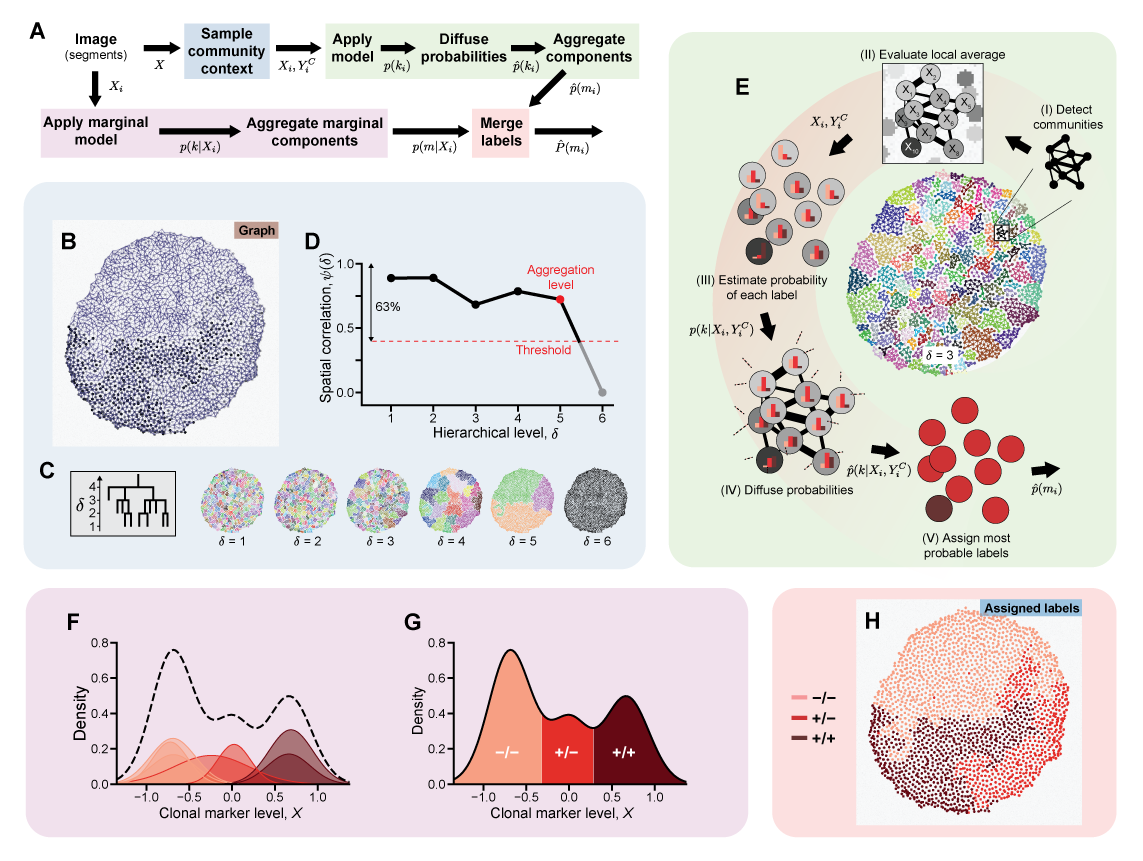
\includegraphics[width=1.0\columnwidth]{./figure_S4}
\caption[Robustness of ribosomopathy simulations to model assumptions.]{\textbf{Reduced protein synthesis capacity diminishes the importance of auxiliary repression over a wide range of model conditions.} Each panel depicts a parameter sweep of the nine-dimensional hyperspace defined by one order of magnitude variation in each of the respective model parameters. For each parameter set, error frequency and percent overexpression were calculated as previously described. They pertain to 50\% reduced repression mimicking auxiliary repressor loss. Error frequency and percent overexpression were calculated independently for conditions of normal and reduced protein synthesis. The difference in error frequency or overexpression between metabolic conditions are shown color-coded, e.g. blue indicates error suppression by reduced protein synthesis. (A-C) Simulations in which the duration of the stimulus input is constant. Shown are the (A) differential error frequencies and (B) differential changes in expression dynamics relative to normal protein synthesis conditions. (C) Differential error frequencies for varying definitions of the success threshold. Each line represents one parameter set, colored by the corresponding range of differential error frequencies. (D) Simulations where a nonzero basal stimulus is applied. (E) Simulations where input duration is increased two-fold by a reduction in protein synthesis capacity. (F) Simulations when an upper bound is placed on the number of sites firing transcription. (G) Simulations when cooperative transcription kinetics are considered.}
\label{fig:metabolism:figS4}
\end{figure}


\graphicspath{ {figures/conclusion/} }

%%%%%%%%%%%%%%%%%%%%%%%%%%%%%%%%%%%

\chapter{Conclusions}
\label{ch:conclusion}

The preceding chapters explore how the structure and function of gene regulatory networks control cell fate decisions and yield emergent properties at the organismal scale. Each chapter individually advances the fields of systems and developmental biology in unique ways.

Chapter \ref{ch:clones} introduced a computational framework for automated analysis of genetic mosaics; a class of experiments commonly used to probe cell fate decisions \textit{in situ} \cite{Germani2018,Atkins2019}. The framework combines computer vision and statistics to automate the labor-intensive steps of a quantitative work-flow, enabling automated and systematic comparison of cells subject to control and perturbation conditions in an otherwise equivalent background.

Quantitative mosaic analysis itself is not new, nor is it uncommon in high profile publications \cite{Dai2017,Gavish2016,Li2018}. Yet, these studies deploy an irreproducible mix of ad hoc implementations and costly commercial software. Worse still, qualitative analysis pervades less prominent corners of the literature. Contributing a fully automated framework to the open-source ecosystem will make quantitative mosaic analysis accessible to the research community as a whole. A unified framework will also dramatically simplify the reproduction of existing analyses. Chapter \ref{ch:clones} therefore advances the quantification of developmental biology by adding potential for rigor and reproducibility where they are currently lacking.

Chapter \ref{ch:ratio} explored a novel cell fate decision mechanism underlying photoreceptor specification in the \textit{Drosophila} larval eye. Computer vision techniques were used to extract quantitative measurements of Pnt and Yan dynamics from a wealth of confocal microscopy data. Statistical analysis revealed that differentiation is driven by dynamic changes in the ratio between Pnt and Yan, and is agnostic to changes in their absolute concentrations as long as the ratio remains constant. The data therefore provide the first direct evidence that cell fate decisions can be triggered by changes in the relative abundance of separate transcription factors. This finding rebukes the canonical model of photoreceptor specification \cite{Graham2010}. More importantly, it adds a new dimension to our understanding of how multiple transcription factors cooperatively control cell fate decisions, with broad implications for many developmental contexts within and beyond \textit{Drosophila}. 

The ratiometric sensing mechanism identified in Chapter \ref{ch:ratio} adds to a growing body of evidence that cells are able to sense relative changes in the abundance of GRN components \cite{Goentoro2009a,Frick2017}. These discoveries are exciting because relative sensing could potentially isolate cell fate decisions from environmental sources of variation. This is because environmental fluctuations would likely manifest as correlated extrinsic noise that affects all GRN components in a similar manner, causing absolute but not relative concentrations to vary between cells. Relative sensing might then increase fitness in variable environments. 

Regulatory interactions may provide additional layers of stability. Dual-reporter experiments have shown that regulation buffers cell-by-cell differences in yeast gene expression to enhance the precision of decisions to commit to a mating response phenotype \cite{Colman-Lerner2005}. Indeed, Chapter \ref{ch:metabolism} also showed that the microRNA miR-7 buffers Yan expression levels, and by extension R cell fate decisions, against varying biosynthesis capacity. Perhaps future experiments could address how Pnt levels are affected before and after IPC ablation in $yan^{\Delta miR\hyphy 7}$ mutants. 

These observations reflect a central theme of this dissertation; the structure and function of developmental GRNs dictate the robustness of cell fate decisions to environmental variation. Chapter \ref{ch:metabolism} directly embraced this sentiment. It proposed a new theory to explain why the regulatory networks that coordinate cell fate decisions often contain many seemingly redundant repressors acting upon the same target genes. The theory posits that auxiliary negative regulators mitigate erroneous cell fate decisions when cells are rapidly metabolizing, and implies that auxiliary repressors may help GRNs adapt their behavior to environmentally driven variation in cell metabolism. The theory is supported by a diverse collection of experiments in which repressor loss-of-function phenotypes were reversed when biosynthesis rates were slowed. A quantitative modeling framework was used to explore the mechanistic origin of this effect, and theoretically demonstrated that auxiliary repressors could avert erroneous decisions by expanding cells capacity to buffer excess protein expression. Quantitative measurements of transcription factor activity confirmed the hypothesized mechanism in vivo.

Chapter \ref{ch:introduction} introduced the notion that developmental GRNs guide organisms through a tortuous journey from embryo to adulthood. The journey is not a sprint. Rather, cells must carefully navigate the many twists and turns of developmental programs; rapidly synthesizing GRN components when and where they are needed, then degrading them with comparable urgency. Protein synthesis and degradation machineries supply the engine and brakes needed to negotiate these obstacles. Individuals stand to benefit from completing the journey quickly because they are generally vulnerable until adulthood, with little means to defend themselves against predation and other dangers. They could naively swap out the engine for something more potent, but added power escalates the risk of perilous consequences. Instead, they could realize the best of both worlds by simultaneously upgrading the brakes. Similarly, organisms may accelerate development by expanding biosynthesis capacity, but the resultant boost in protein expression can cause erroneous cell fate decisions that lead to the emergence of deleterious phenotypes. By simultaneously incorporating additional repressors, they can tolerate faster metabolic rates without compromising the accuracy of cell fate decisions. The data presented in Chapter \ref{ch:metabolism} demonstrate that auxiliary repressors enable faster development by illustrating the inverse perspective. Repressors were shown to be dispensable when metabolism was slow, much in the way that stock brakes would suffice at low speeds. 

This line of reasoning implies that a novel evolutionary driving force may shape the structure and function of developmental gene regulatory networks. Shorter generational times confer a selective advantage beyond reducing individuals exposure during infancy. They facilitate rapid exploration of the phenotypic landscape, enabling fast adaptation to variable environments. GRNs should therefore be expected to incorporate any topological features that allow development to proceed more quickly. The abundance of seemingly redundant regulation found in developmental GRNs certainly appears to support this hypothesis, and thus reinforce our contemporary understanding that robustness is a fundamental organizational principle underlying the evolution of biological systems \cite{Kitano2004,Stelling2004}. 

The findings also contribute to an emerging view that cells capacity to rapidly adjust protein homeostasis directly affects organismal fitness and health \cite{Visscher2016,Tollerson2018,Burnaevskiy2018}. The assertion is backed by convincing experimental evidence. Burnaevskiy et al used a dual-reporter scheme in \textit{C. elegans} to show that cellular differences in the abundance of protein synthesis machinery manifest in the population-wide penetrance of adult phenotypes. The authors went on to speculate that longevity might be similarly be affected \cite{Burnaevskiy2018}. Tollerson et al showed that Elongation factor P alleviates a translational bottleneck caused by ribosomal queuing in \textit{E. coli}, facilitating adaption to environmentally-driven increases in cell metabolism \cite{Tollerson2018}. Chapter \ref{ch:metabolism} contributes unique evidence that the accuracy of cell fate decisions depends upon cells ability to dynamically balance the push and pull of protein synthesis and degradation. 

% ================================================ FUTURE DIRECTIONS
\section{ Avenues for further exploration }

This dissertation prompts several exciting new directions for future research. This section begins with a survey of those that merit further attention, before elaborating on some preliminary analyses to guide prospective efforts.

Chapter \ref{ch:ratio} proposed that R cell fate commitment in the larval eye is driven by dynamic changes in the relative abundance of Pnt and Yan. Experimental evidence was limited to correlative observations because intrinsic regulation precluded direct manipulation of the Pnt-to-Yan ratio by varying gene dosage. Future studies could rigorously confirm the hypothesis by applying the same gene dosage perturbations in a genetic background that lacks the complete set of regulatory interactions needed to stabilize the Pnt-to-Yan ratio. Disrupting the ratio control mechanism would first require characterizing its biomolecular implementation. Computational simulations could explore the space of plausible GRN topologies, then leverage insight derived from existing experimental data to distill a manageable number of options for experimental validation. Establishing an unambiguous picture of R cell fate commitment might then allow for a complete model of retinal patterning dynamics, as is an ongoing mission among computational biologists \cite{Lubensky2011,Gavish2016}.

Chapter \ref{ch:ratio} used an equilibrium modeling framework to explore the effect of \textit{cis}-regulatory interactions between Yan monomers on the equilibrium binding occupancy of promoters regulated by Pnt and Yan. The approach was inspired by the work of Hope et al, who used an equivalent model, limited to a single binding component, to explore how the \textit{cis}-regulatory syntax of target genes modulates transcriptional output \cite{Hope2017}. The multi-species implementation introduced in Chapter \ref{ch:ratio} was comparatively underutilized. Future studies could ask many questions related to how \textit{cis}-regulatory syntax modulates the transcriptional output of genes regulated by two or more polymerizing transcription factors. How do the number and arrangement of individual binding sites modulate transcriptional output? What about the spacing or distribution of high and low affinity sites? What if anti-cooperative or steric interactions are included? Does the number of unique binding species matter? All of these questions could readily be explored using the open-source platform developed to support this dissertation (see Appendix \ref{appendix:software}).

The theory developed in Chapter \ref{ch:metabolism} posits that auxiliary repressors stabilize cell fate decisions against environmental variation in cells capacity to synthesize and degrade proteins. This assertion was backed by both experiments and computational analysis showing that repressors were dispensable when either ATP turnover or translation capacity were reduced. It is well known that many mutant phenotypes are also suppressed in animals raised at low temperatures. Future studies could ask whether reduced temperature imparts similar effects on the GRN dynamics that govern cell fate decisions. From a modeling perspective, the primary challenge would be deciding precisely how to incorporate the relative effects of temperature on the protein synthesis and degradation machineries. The analogous decisions were comparatively obvious for \textit{ILP2-GAL4 UAS-Rpr} and \textit{RP} mutants, in which protein synthesis is disproportionately affected. In principle, experimental efforts to quantify the dependence of protein synthesis and degradation rates on temperature could prove fruitful.

Alternatively, researchers could computationally survey the landscape of plausible relationships between proteostasis and the environment to identify conditions under which auxiliary repressors are dispensable. For instance, consider the simplest possible model of protein expression dynamics (Fig. \ref{fig:conc:fig1}A):
\begin{equation}
\label{eq:simple_base}
\frac{dP}{dt} = kI - \gamma P
\end{equation}
where $P$ and $I$ are the protein and stimulus levels, and $k$ and $\gamma$ are the synthesis and degradation rate parameters. Repressors may be implemented as proportional feedback, as they were in Chapter \ref{ch:metabolism}:
\begin{equation}
\label{eq:simple_repressor}
\frac{dP}{dt} = kI - \gamma P - \eta P
\end{equation}
where $\eta$ is the feedback strength. The frequency of developmental errors induced by losing the repressor is readily evaluated using the same procedure described in Chapter \ref{ch:metabolism} (Fig. \ref{fig:conc:fig1}B). Rather than hard-coding an explicit dependence of $k$, $\gamma$, and $\eta$ on environmental conditions, each parameter can be scaled by a latent dimension $\lambda$ that reflects the environmental state of the cell:
\begin{equation}
\begin{aligned}
k &\propto \lambda^{\nu_k}  \\
\gamma &\propto \lambda^{\nu_{\gamma}}  \\
\eta &\propto \lambda^{\nu_{\eta}}
\end{aligned}
\label{eq:parameter_dependence}
\end{equation}
where $\nu_k$, $\nu_{\gamma}$, and $\nu_{\eta}$ define the respective sensitivities of synthesis, degradation, and feedback strength to environmental conditions. Consider an example in which the environmental state of the cell is halved relative to some reference condition, i.e. $\lambda = \lambda_{0} / 2$. For $\nu_{i \in {k,\gamma,\eta}} = 1$, parameter $i$ is also halved. If $0 < \nu_i < 1$ or $\nu_i > 1$, parameter $i$ exhibits sub- or super-linear dependence on the environment, respectively. Finally, $\nu_i < 0$ implies that parameter $i$ should actually increase when $\lambda$ is halved. 

The robustness checks presented in Section \ref{metabolism:robust} surveyed a handful of discrete values for the model parameters analogous to $\nu_k$, $\nu_{\gamma}$, and $\nu_{\eta}$. The scaling assumptions used to represent conditions of reduced energy metabolism throughout Chapter \ref{ch:metabolism} were loosely equivalent to $(\nu_k, \nu_{\gamma},\nu_{\eta}) = (1,0,2)$. Applying the same assumptions to the simplified model recapitulates a core result of Chapter \ref{ch:metabolism}; error frequency is dependent upon the environmental state of the cell (Fig. \ref{fig:conc:fig1}C,D).

\begin{figure}[h!]
\centering
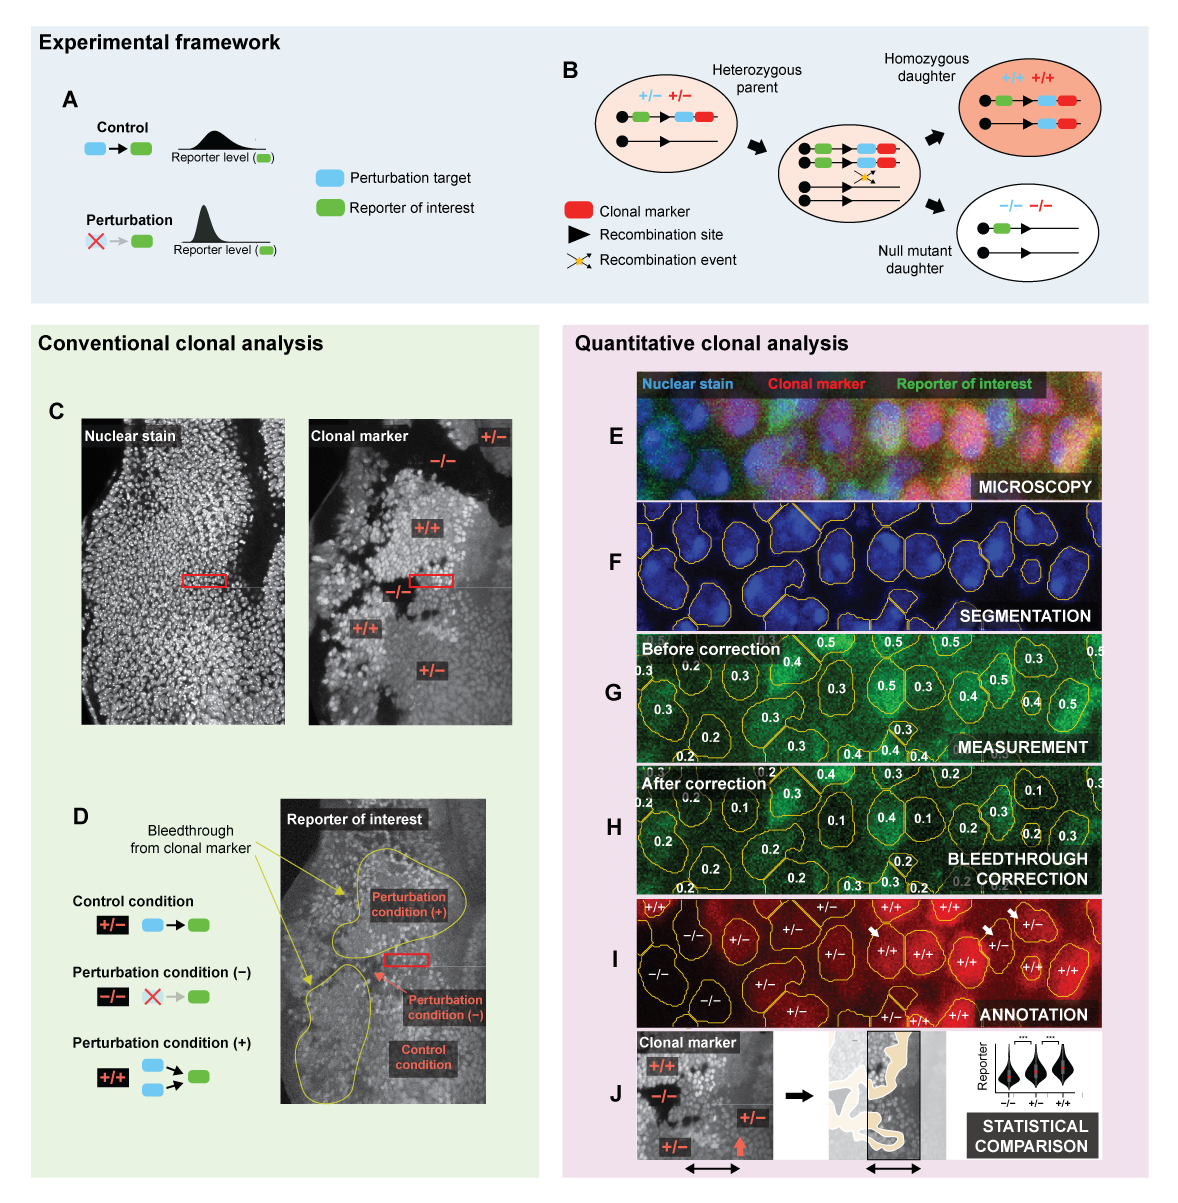
\includegraphics[scale=1.0]{./figure_1}
\caption[Simplified framework for modeling the loss of an auxiliary repressor.]{\textbf{Simplified framework for modeling the loss of an auxiliary repressor.} (A) Schematic representation of protein expression in response to a transient input. Output is subject to regulation by a single auxiliary repressor. (B) Simulated emergence of developmental errors. Simulations may be performed with (purple) or without (grey) the auxiliary repressor. Lines reflect a random sample of 5000 trajectories. The two sets of trajectories are compared when 99\% of trajectories simulated with the repressor cross a threshold value (dashed line). Without the auxiliary repressor, very few trajectories successfully cross the threshold. (C) Graphic representation of the relation between environmental conditions and the rate parameters that dictate protein synthesis, degradation, and repressor strength. (D) Error frequency is dramatically suppressed by a change in environmental conditions. }
\label{fig:conc:fig1}
\end{figure}

Combined, equations \ref{eq:simple_repressor} and \ref{eq:parameter_dependence} facilitate continuous enumeration of the phase diagram spanned by $\nu_k$, $\nu_{\gamma}$, and $\nu_{\eta}$ in order to identify the range of scaling assumptions under which auxiliary repressors may be dispensable. Performing this exercise revealed that induced error frequencies are highest when the strength of the removed repressor is more sensitive to the environment than the intrinsic rate of protein turnover (Fig. \ref{fig:conc:fig2}A, region IV). The same is true of error frequency suppression, indicating that highly sensitive repressors have the highest propensity to become dispensable (Fig. \ref{fig:conc:fig2}B, region IV). This observation is consistent with intuition, as environmental conditions that limit the influence of a repressor would also be expected to mitigate the impact of its removal. 

This preliminary analysis could guide the design of future experiments that survey the effects of temperature on mutations that compromise repressor function. For example, experiments could quantify $\nu_k$, $\nu_{\gamma}$, and $\nu_{\eta}$ for a particular cell-fate determinant by measuring steady-state protein levels in both wildtype and repressor loss-of-function mutants across a range of temperatures. They could then use the model to generate testable predictions for alternate temperatures.

\begin{figure}[h!]
\centering
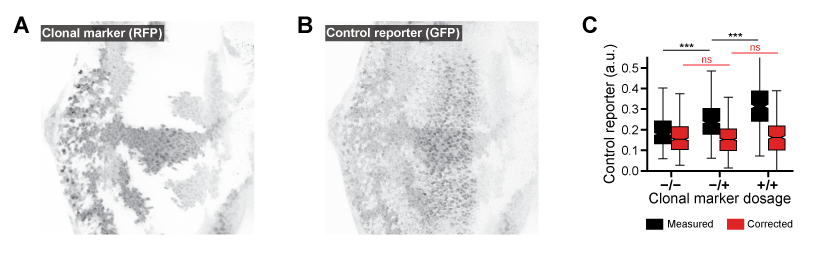
\includegraphics[scale=1.0]{./figure_2}
\caption[Environmental sensitivities under which auxiliary repressors are dispensable.]{\textbf{Environmental sensitivities under which auxiliary repressors are dispensable.} Phase diagrams span a range of assumptions regarding the relative sensitivity of protein degradation and feedback strength to environmental conditions. Heatmaps show (A) error frequency induced by the loss of an auxiliary repressor when $\lambda = \lambda_0$ and (B) change in error frequency when $\lambda = \lambda_0 / 2$. All simulations use $k = 1$, $\gamma = 0.001$, $\eta = 0.001$, and $\lambda_0 = 1$. Dark blue indicates strong error frequency suppression. Red numerals label quadrants. The example shown in Fig. \ref{fig:conc:fig1} is taken from quadrant IV. }
\label{fig:conc:fig2}
\end{figure} 

Chapter \ref{ch:metabolism} also raises the question of whether any other features of GRNs are dispensable under certain environmental conditions. For instance, how about promoters? Preliminary analysis may again provide some insight to guide future work. Consider another scenario in which an auxiliary promoter is added to the simple model given by Equation \ref{eq:simple_base}:
\begin{equation}
\label{eq:simple_promoter}
\frac{dP}{dt} = kI + k_{aux}I - \gamma P
\end{equation}
where $k_{aux}$ is the rate constant for synthesis driven by the auxiliary promoter. The relative influence of the auxiliary promoter is given by its strength relative to the primary promoter, i.e. $log_2 ( k_{aux} / k )$. The respective sensitivities of both promoters and degradation to environmental conditions are again parameterized in terms of $\lambda$:
\begin{equation}
\begin{aligned}
k &\propto \lambda^{\nu_k} \\
k_{aux} &\propto \lambda^{\nu_{k-aux}} \\
\gamma &\propto \lambda^{\nu_{\gamma}} \\
\end{aligned}
\end{equation}
The simulation procedure described in \ref{ch:metabolism} is readily modified to evaluate the frequency of developmental errors induced by removing the auxiliary promoter, i.e. by setting $k_{aux}=0$. Intuition suggests promoter loss should cause a decrease in output protein levels. Error frequency is therefore redefined to reflect the extent to which protein is \emph{under-expressed} when the auxiliary promoter is removed. The metric is evaluated by computing the fraction of trajectories simulated with a single promoter that fail to reach the lower bound of trajectories simulated with both promoters. Surveying a range of promoter strengths and relative influences reveals that error frequencies are most severe when strong and influential auxiliary promoters are removed (Fig. \ref{fig:conc:fig3}A). Figure \ref{fig:conc:fig3}B shows the subsequent change in error frequencies when $(\nu_k, \nu_{k-aux},\nu_{\gamma}) = (1,1,1)$ and $\lambda = \lambda_0 / 2$. The phase diagram is punctuated by a diagonal band in which error frequencies are suppressed. Below this band, suppression is minimal because the auxiliary promoter is inconsequential to normal protein expression dynamics (Fig. \ref{fig:conc:fig3}A,B, region I). Above it, removing the auxiliary promoter imparts a severe perturbation that cannot be recovered by the proposed change in environmental conditions (Fig. \ref{fig:conc:fig3}A,B, region II). Similar zones arise when the equivalent procedure is performed using the model of auxiliary repressor loss defined by equation \ref{eq:simple_repressor} (Fig. \ref{fig:conc:fig4}). Here, the influence of the auxiliary repressor is defined relative to the intrinsic degradation rate, i.e. $log_2 ( \eta / \gamma )$. 

\begin{figure}[h!]
\centering
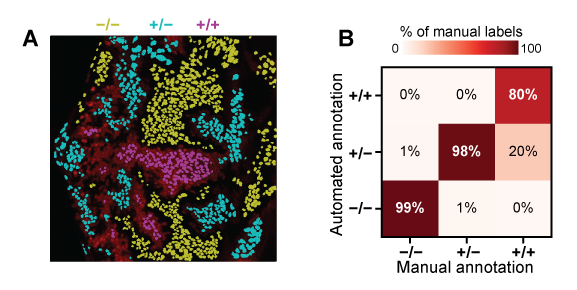
\includegraphics[scale=1.0]{./figure_3}
\caption[Phase diagram of auxiliary promoter loss.]{\textbf{Phase diagram of auxiliary promoter loss.} 
Phase diagrams span a range of auxiliary promoter strengths and influences. Heatmaps show (A) error frequency induced by the loss of the auxiliary promoter when $\lambda = \lambda_0$ and (B) change in error frequency when $\lambda = \lambda_0 / 2$. All simulations use $\gamma = 0.001$ and $\lambda_0 = 1$. Dark blue indicates strong error frequency suppression. Perturbations targeting promoters in region I are inconsequential. Those targeting promoters in region II are too severe to be recovered. Blue band is the Goldilocks zone.}
\label{fig:conc:fig3}
\end{figure}

\begin{figure}[h!]
\centering
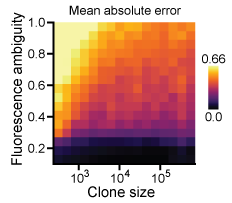
\includegraphics[scale=1.0]{./figure_4}
\caption[Phase diagram of auxiliary repressor loss.]{\textbf{Phase diagram of auxiliary repressor loss.} 
Phase diagrams span a range of auxiliary repressor strengths and influences. Heatmaps show (A) error frequency induced by the loss of the auxiliary repressor when $\lambda = \lambda_0$ and (B) change in error frequency when $\lambda = \lambda_0 / 2$. All simulations use $k = 1$ and $\lambda_0 = 1$. Dark blue indicates strong error frequency suppression. Perturbations targeting repressors in region I are inconsequential. Those targeting repressors in region II are too severe to be recovered. Blue band is the Goldilocks zone.}
\label{fig:conc:fig4}
\end{figure}

The bands observed in Figures \ref{fig:conc:fig3}B and \ref{fig:conc:fig4}B indicate the existence of a Goldilocks zone in which perturbations are strong enough to be felt but weak enough to be recoverable. In other words, there exists a finite and continuous range of conditions in which error frequencies can be suppressed by slowing biosynthesis. Given appropriate knowledge of promoter and repressor strengths, a model could inform the selection of experimental perturbation targets that fall within the range. Such an approach would also require quantification of $\nu_i$ and $\lambda$ for a given model system.

The value of the models defined by equations \ref{eq:simple_repressor} and \ref{eq:simple_promoter} lies in their simplicity. Because each strictly employs linear kinetics, the stochastic dynamics are analytically tractable via a closed system of moment equations \cite{Sotiropoulos2011}. While numerical simulations were used to perform the analysis presented in this section, future theoretical efforts could be directed toward the development of a rigorous analytical framework.

% ================================================ PERSPECTIVES ON QUANT BIO
\section{Perspectives for quantitative biology}

This dissertation surveyed developmental cell fate decisions through a quantitative lens. It used numbers and equations to derive nuanced understanding from processes that are notoriously difficult to characterize. In many cases, doing so required forcible reconciliation with time-honored traditions in biological analysis. Two major obstacles encountered along the way merit further discussion.

First, models should fit the data; not the other way around. While it may be possible to coax data into a conventional framework, tailoring one appropriate for the task at hand will generally return more meaningful insight. Mathematical flexibility was a key strength of this dissertation. Each chapter leveraged a customized modeling framework to tease deeper meaning out of experimental data than would otherwise have been possible using conventional techniques. 

Chapter \ref{ch:clones} deployed a Bayesian statistical framework to infer cell genotypes from an image of clonal marker expression. Biological intuition suggests it should have enforced detection of three distinct components strictly delimited by clonal marker level. Instead, the model was designed to tolerate an arbitrary number of components that also considered spatial context, which were later aggregated into the three anticipated genotypes. This empirical formulation buffered uncertainties imparted by expression heterogeneity and imaging noise to improve annotation performance overall.

Chapter \ref{ch:ratio} used an equilibrium binding model to explore how \textit{cis}-regulatory interactions between Yan monomers bias the transcriptional output of genes simultaneously regulated by Pnt. Conventional wisdom suggests a competitive binding model using the Hill-Langmuir equation would be appropriate \cite{Gesztelyi2012}. Instead, a statistical mechanical approach was adapted from earlier work by Hope et al \cite{Hope2017}. Contrary to the empirical strategies used in other chapters, this model substantially \emph{increased} the resolution of analysis. Doing so granted detailed mechanistic insight into the intricacies of polymerizing transcription factors, which would have otherwise been inaccessible (see Fig. \ref{fig:ratio:figS5}C). 

Chapter \ref{ch:metabolism} sought to model the dynamic output of GRNs controlling a broad spectrum of cell fate decisions. The conventional first step would have been to identify and consolidate all known regulatory interactions in each system. Such an endeavor was certainly possible for Yan-mediated control of retinal patterning, as the pertinent interactions have been studied for decades \cite{Ready1976a,Rebay1995,Rohrbaugh2002,Li2009b,BoisclairLachance2014} and in some cases quantified \cite{Pelaez2015a}. Chapter \ref{ch:metabolism} instead drew inspiration from control theory to develop a model strictly concerned with the two salient features of pulsatile dynamics; the magnitude of induction and timescale of decay. The model jettisoned the molecular details of protein expression and regulation in each system, instead favoring a coarse-grained depiction of output dynamics. The reductionist approach was vital to the model's ability to simultaneously depict the behavior of a diverse assortment of cell fate decisions.

The model deployed in Chapter \ref{ch:metabolism} also surmounted the second major obstacle: The resolution of analysis should match the resolution of the data. Biological networks are complex, often far more complex than we can intuitively comprehend. Their emergent behavior arises from the collective interactions of numerous components, many of which are often unknown. These uncertainties make it particularly dangerous to represent systems-level behavior by the sum of its parts. Similarly, predictions are all but meaningless when made by aggregating disparate interactions that were characterized in isolation.

Despite their pitfalls slowly coming under scrutiny, these practices remain tragically common. They are perhaps most strongly embodied in the abundance of cartoons that purport to depict systems level-behavior with a compendium of qualitative regulatory interactions. Figure \ref{fig:ratio:fig7}A provides a modest example. This cartoon is harmless by itself, but problems arise when unsuspecting viewers ascribe physical meaning to the various interactions. After all, there is no unified standard to define what these arrows mean. A single arrow might actually represent an entire sub-network of complex nonlinear processes. Intermediate steps within an arrow might even interact with other intermediates in separate arrows drawn elsewhere in the diagram. Cartoons are thus rife with ambiguity that hinders the communication of otherwise outstanding research. For instance, a basic attempt to simulate the system shown in Figure \ref{fig:ratio:fig7}A revealed that the illustrated ``regulatory loop'' cannot maintain a constant Pnt-to-Yan ratio in response to varying \textit{pnt} or \textit{yan} gene dosage (results not shown).

This ambiguity starkly contrasts the standardized descriptive languages commonly used in engineering \cite{Lazebnik2004}. But, to be fair, most human-engineered systems do not suffer the same extent of uncertainty as their biological counterparts. Notable exceptions arise in electrical, chemical, and biomolecular engineering. Autonomous vehicles, advanced robotics, process plants, and synthetic biological circuits must all contend with disturbances whose origin and character may be unpredictable or unknown. Fortunately, a viable solution to this challenge already exists. Control theory emphasizes an empirical representation of systems-level dynamics that is easily matched to the resolution of available information \cite{Seborg2011}. In many cases, the detailed internal system dynamics may remain unknown. Sensors need only monitor the minimum set of process variables necessary to ensure that a given process is controllable. Often, this simply entails monitoring systems-level output and taking corrective action when it deviates from a desired set point. 

Control theory offers a particularly compelling perspective for rationalizing the behavior of developmental GRNs. Most are inherently localized in time, contain numerous unknown components and interactions, and ultimately coordinate a manageable number of outputs. This rationale inspired the conceptual model of ratiometric control used to interpret the R cell fate decision analyzed in Chapter \ref{ch:ratio}. After all, Pnt and Yan are transiently expressed, subject to extensive uncharacterized regulation, and appear to mediate R cell fate transitions through a single observable output; the Pnt-to-Yan ratio. Similar reasoning inspired the modeling framework used throughout Chapter \ref{ch:metabolism}. The breadth of experiments pointed toward a dynamic phenomenon agnostic to the molecular detail of repressors and their targets. Furthermore, among all systems surveyed, only Yan and Sens expression were measurable. The resolution of analysis was therefore matched to the resolution of the data by modeling the representative dynamics of a generic protein, subject to feedback at each of the three levels that were experimentally surveyed (see Fig. \ref{fig:metabolism:figS1a}). Combined, these approaches contribute unique perspectives to the growing trend of interpreting biological robustness through the eyes of control theory \cite{Khammash2016}. 

As biology and engineering converge on common interests, it is important to reconcile the strengths of both disciplines. Biology contributes a wealth of prior knowledge and experimental techniques that frequently bewilder even the most seasoned engineers. Engineering contributes quantitatively rigorous frameworks to systematically analyze, interpret, predict, and design complex systems. The promise of a successful integration prompts continued dialogue to resolve any growing pains and advance the field of quantitative biology as a whole.


% bibliography
\begin{singlespace}
\bibsep 10pt
\bibliography{./bib/thesis}
\bibliographystyle{unsrtnat}
\end{singlespace}

% appendix
\appendix
\chapter{Supporting information for Chapter \ref{ch:ratio}}
\label{appendix:ratio}
\graphicspath{ {./figures/ratio/} }

%%%%%%%%%%%%%%%%%%%%%%%%%%%%%%%%%%%

The experiments detailed in this section were conceived, designed, and conducted by my collaborators, most notably Nicol'{a}s Pel'{a}ez and Jean-Francois Boisclair Lachance. They are included here for completeness.

\section{Genetics}
\label{appendix:ratio:genetics}

The recombineered \textit{pnt-gfp} BAC transgene inserted into the VK00037 landing site was previously described in Boisclair-Lachance et al. (2014). Alleles $pnt^{\Delta 88}$ \cite{ONeill1994a} and $pnt^2$ (Bloomington Stock 2222) were used to render the endogenous \textit{pnt} gene null in the presence of \textit{pnt-gfp}. A single copy of \textit{pnt-gfp} rescued $pnt^{\Delta 88}/pnt^2$ to full viability and fertility (Fig. \ref{fig:ratio:figS1}A). Cell nuclei of developing eye-antennal discs were marked by recombining \textit{H2Av-mRFP} (Bloomington stock 23651) with $pnt^2$. Experiments measuring wild type dynamics of \textit{Pnt-GFP} were done by dissecting eye discs from white prepupae carrying $w^{1118}$ ; $pnt\hyphy gfp / pnt\hyphy gfp$ ; $pnt^{\Delta 88}/pnt^2$, $H2Av\hyphy mRFP$. \textit{Pnt} isoform-specific expression was detected using enhancer traps \textit{HS20} (gift from B. Shilo) and $pnt^{1277}$ (Bloomington stock 837), which report \textit{PntP1} and \textit{PntP2} transcription respectively by expressing LacZ \cite{Scholz1993}. \textit{pnt-gfp} and \textit{pnt} isoform-specific expression were compared in white prepupae carrying $w^{1118}$; $pnt\hyphy gfp/pnt\hyphy gfp$; $HS20/+$ and $w^{1118}$;$pnt\hyphy gfp/pnt\hyphy gfp$; $pnt^{1277}/pnt^{1277}$. \textit{Pnt} gene dosage experiments were done using $w^{1118}$; $pnt\hyphy gfp/+$ ; $pnt^{\Delta 88}/pnt^2$ (1x pnt) and $w^{1118}$; $pnt\hyphy gfp/pnt\hyphy gfp$ ; $pnt^{\Delta 88}/pnt^2$ (2x pnt). Notch activity was conditionally reduced using the $N^{ts1}$ temperature sensitive allele \cite{Shellenbarger1975}. $N^{ts1}/N^{ts1}$ ; $pnt\hyphy gfp/+$ animals were raised at the permissive temperature (18 \textdegree{}C) and shifted to the restrictive temperature (28.5 \textdegree{}C) as third instar larvae for 24 h. Animals exposed to the restrictive temperature that were transferred back to the permissive temperature had roughened eye phenotypes and a notched wing phenotype as adults, consistent with effective inhibition of Notch activity. Control larvae of the same genotype were grown at the permissive temperature until dissection. Both control and heat-treated larvae were sexed and only \textit{N} hemizygote males carrying $N^{ts1}/Y$ ; $pnt\hyphy gfp/+$ were dissected as white prepupae. EGFR activity was conditionally reduced by placing the null allele $egfr^{f24}$ - also known as $egfr^{CO}$ \cite{Clifford1989} \textit{in trans} to the thermo-sensitive allele $egfr^{tsla}$ \cite{Kumar1998}, as previously described \cite{Pelaez2015a}. The genotype was $w^{1118}$; $egfr^{tsla}$, $pnt\hyphy gfp/egfr^{24}$, $pnt\hyphy gfp$. Ras activation was achieved using a transgene expressing a $Ras1^{V12}$ mutant and driven by a 3x\textit{sev} enhancer and promoter \cite{Fortini1992} as previously described \cite{Pelaez2015a}. \textit{Pnt-gfp} in the Ras mutant background was measured using $w^{1118}$; $pnt\hyphy gfp$, $Sev>Ras^{v12}/pnt\hyphy gfp$;$pnt^2$,$H2Av\hyphy mRFP/+$. Controls animals carried $w^{1118}$; $pnt\hyphy gfp/pnt\hyphy gfp$, $pnt^2$, $H2Av\hyphy mRFP/+$. \textit{Yan} mutant eye clones were generated using the $yan^{833}$ null allele \cite{Webber2013}, \textit{ey$>$FLP} and the FRT40 crossover point. $Pnt^+$ tissue was labeled using the clonal marker $Ubi>mRFP_{nls}$ (Bloomington Stock 34500). Developing eyes were dissected from white prepupae carrying $w$, $ey>FLP$; $pnt\hyphy gfp$, $yan^{833}$, $FRT40A/pnt\hyphy gfp$, $Ubi>mRFP_{nls}$, $FRT40A$. Control discs to measure the GFP-mRFP fluorophore bleed-through were obtained from flies carrying $w$, $ey>FLP$; $pnt\hyphy gfp$, $Ubi>mRFP_{nls}$, $FRT40A/pnt\hyphy gfp$, $FRT40A$ or $w$, $ey>FLP$; $pnt\hyphy gfp$, $Ubi>mRFP_{nls}$, $FRT40A/CyO$.

\section{Immunohistochemistry}
\label{appendix:methods:ratio:immunohistochemistry}

Unless otherwise noted, Pnt-GFP and Yan were measured in developing animals raised at 21 \textdegree{} C, selected as white prepupae, and subsequently aged in humid chambers for 5-10 h. Eye-antennal discs were dissected in PBS, and fixed in 4 \% (w/v) paraformaldehyde/PBS for $\sim$45 min. Endogenous Yan protein was detected with the mouse monoclonal anti-Yan antibody 8B12 (Developmental Studies Hybridoma Bank, 1:200 dilution) and the secondary goat anti-mouse Pacific Blue antibody (Life Technologies, 1:200 dilution). Expression from the \textit{HS20} and $pnt^{1277}$ enhancer traps was detected using mouse anti-$\beta$-galactosidase 40-1a (Developmental Studies Hybridoma Bank, 1:50 dilution). H2Av-mRFP was used as a nuclear marker as previously described in Pel\'{a}ez et al. (2015). Discs were incubated in 1:1 (v/v) PBS:VectaShield (Vector Laboratories) for 45 min, then in 100\% VectaShield for an additional 45 min before mounting.

For experiments using \textit{yan} mutant clones, $N^{ts}$, or $EGFR^{ts}$ alleles, nuclei were stained with a 4',6-diamidino-2-phenylindole (DAPI) nuclear marker. Samples were fixed in 4\% paraformaldehyde, rinsed with PBS-Tween 0.5\%, and permeabilized with PBS-Triton X-100 0.1\% for 20 minutes at room temperature. Permeabilization was important to allow DAPI penetration without perturbing the fluorescence of the Pnt-GFP protein. After permeabilization, eye discs were incubated in a blocking solution containing PBS-Tween 0.1\% and 1\% normal goat serum for 30 minutes at room temperature. Primary and secondary antibodies were incubated each for 2 hours at room temperature. Antibodies used with DAPI were: mouse anti-Yan 8B12 (DHSB, 1/500) and goat anti-mouse Cy3 (1/2000, Jackson Immunoresearch). Discs were mounted in 0.5\% n-propyl-gallate, 0.1M Tris pH 8.0 and 90\% glycerol.

Samples were kept in the dark at -20 \textdegree{}C and imaged no later than 18-24 hr after fixation. In all cases, 1024 x 1024 16-bit images were captured using either a Zeiss LSM880 or a Leica SP5 confocal microscope equipped with 40X oil objectives. During imaging, discs were oriented with the equator parallel to the x-axis of the image. Optical slices were set at 0.8µm slices (45-60 optical slices) with an additional digital zoom of 1.2-1.4 to completely image eye discs from basal to apical surfaces. Images recorded a region of at least 6 rows of ommatidia on each side or the dorsal-ventral eye disc equator. All discs for a given condition were fixed, mounted, and imaged in parallel to reduce measurement error.

\graphicspath{ {./figures/ratio/} }

%%%%%%%%%%%%%%%%%%%%%%%%%%%%%%%%%%%

\section{Quantification of expression levels}
\label{appendix:ratio:quantification}

Expression dynamics were inferred from confocal image stacks using an updated version of an existing segmentation and annotation pipeline \cite{Pelaez2015a}. The new pipeline includes \textit{FlyEye Silhouette}; an open-source package for macOS that integrates our image segmentation algorithm with a GUI for cell type annotation. Subsequent analysis and visualization procedures were implemented in Python.

In all cases, cell segmentation was performed using either H2Av-mRFP or DAPI signals as a reference channel for identification of cell nuclei boundaries. Each layer of the reference channel was segmented independently. A single contour containing each unique cell was manually selected and assigned a cell type using a custom graphic user interface. DAPI-stained discs were segmented using a separate script based on the watershed algorithm in order to mitigate the effect of bright spots caused by DAPI accumulation in nucleoli. Further care was taken to avoid annotating contours containing such nucleoli. For each annotated cell contour, expression measurements were obtained by normalizing the mean fluorescence of the Pnt-GFP and Yan antibody channels by the mean fluorescence of the reference channel. This normalization serves to mitigate variability due to potentially uneven sample illumination, segment area, and in the case of His-RFP, differences in protein expression capacity between cells.

\section{Conversion of distance to time}
\label{appendix:ratio:distance_to_time}

Cell positions along the anterior-posterior axis were mapped to developmental time as described previously \cite{Pelaez2015a,Pelaez2016}. This is predicated on two assumptions: the furrow proceeds at a constant rate of one column of R8 neurons per two hours, and minimal cell migration occurs. We find no reason to discard these assumptions.

For each disc, Delaunay triangulations were used to estimate the median distance between adjacent columns of R8 neurons \cite{Fortune1992}. We used the median rather than the mean distance, as was used in our previous study, because it minimized the influence of non-adjacent R8s that were falsely identified by the triangulation. Dividing the furrow velocity of 2 h per column by this median distance yields a single conversion factor from position along the anterior-posterior axis to developmental time. This factor was applied to all cell measurements within the corresponding disc, yielding expression time series. Notably, these are not single cell dynamics, but rather aggregate dynamics across the development time course of a cell population.

\section{Computation of moving averages and confidence intervals}
\label{appendix:ratio:moving_averages}

Moving averages were computed by first-order Savitzky-Golay filtration \cite{Savitzky1964}. This method augments the simple windowing approach used in our previous study \cite{Pelaez2015a} by enabling visualization of expression trends at early time-points that are otherwise obscured by large window sizes. A secondary first-order filtration with one-fifth the original window size was applied to smooth lines for visualization purposes.

None of our conclusions are sensitive to our choice of filtration or smoothing method \cite{Pelaez2015a}. Primary window sizes of 250 and 75 cells were used for reporting the expression of multipotent and differentiated cells, unless noted otherwise. Confidence intervals for the moving average were inferred from the 2.5th and 97.5th percentile of 1000 point estimates of the mean within each window. Point estimates were generated by bootstrap resampling (with replacement) the expression levels within each window.

\section{Alignment of expression data}
\label{appendix:ratio:alignment}

Cells were aligned with a reference population by shifting them in time. The magnitude of this shift was determined by maximizing the cross-correlation of progenitor Pnt-GFP expression $Y(t)$ with the corresponding reference time series $X(t)$. Rather than raw measurements, moving averages within a window of ten cells were used to improve robustness against noise. This operation amounts to:
\begin{equation}
z = \argmax_{dt} \ {\hat{\gamma}_{X(t),Y(t)}}
\end{equation}
\begin{equation}
\hat{\gamma}_{X(t),Y(t)} (dt) = E \Big[ \frac{(Y(t+dt)-\mu_Y)(X(t+dt)-\mu_X)}{\sigma_Y \sigma_X} \Big]
\end{equation}
where, $\mu$ and $\sigma$ are the mean and standard deviation of each time series, and $dt$ is the time by which the population should be shifted.

For each experimental treatment, a disc was randomly chosen and shifted in time such that time zero corresponds to the first annotated R8 neuron. This disc then served as the reference population for the alignment of all subsequent biological replicates within the treatment. Similarly, different experimental treatments (e.g. control and perturbation) were aligned by first aligning the discs within each treatment, then aggregating all cells within each treatment and repeating the procedure with the first treatment serving as the reference.

This approach differs from the previous implementation of our pipeline in which discs were manually aligned by the inflection point of their Yan-YFP expression profiles \cite{Pelaez2015a}. Manual alignment entails arbitrary prioritization of certain dynamic features over others. Our revised protocol yields consistent, reproducible alignment of expression time series that equally weighs the entire time course. The automated approach is more principled but less robust than the manual approach. Specifically, it fails when dynamic forms qualitatively differ between experimental treatments. In these instances, we revert to manual alignment using the inflection point of Pnt-GFP induction as a reference.

\section{Analysis of \textit{yan} clones}
\label{appendix:ratio:clones}

We used \textit{ey$>$FLP} and \textit{FRT40A} to generate $yan^{833}$ null clones within 23 eye discs carrying the Pnt-GFP transgene (see Section \ref{appendix:ratio:genetics}). The chromosome carrying the wildtype \textit{yan} allele was marked with a Ubi-mRFPnls transgene, enabling automated detection of subpopulations with distinct \textit{yan} gene dosages, each characterized by a distinct level of mRFP fluorescence. Discs were dissected, fixed, and co-stained with DAPI prior to confocal imaging. Images of 36 unique vertical cross-sections spanning non-overlapping cells were collected in total. 

We deployed the framework developed in Chapter \ref{ch:clones} to measure the expression level of each reporter in each nucleus and automatically label each measurement as mutant, heterozygous, or homozygous for the Ubi-mRFPnls clonal marker. For each segment, Ubi-mRFPnls and Pnt-GFP fluorescence was quantified by normalizing the average intensity of all pixels within the respective fluorescence channel by the average DAPI fluorescence. Segments containing less than 250 pixels were removed. 

Fluorescence bleedthrough between the RFP and GFP channels was visually apparent in these discs. To confirm our suspicion, control clones were generated in six wildtype \textit{yan} eye discs co-expressing Ubi-mRFPnls and Pnt-GFP. These are the same discs as those analyzed in Chapter \ref{ch:clones}. We used the correction strategy presented in Section \ref{ch:clones:correction} to systematically correct for bleedthrough from the Ubi-mRFPnls reporter into the GFP channel. The correction successfully eliminated any detectable difference in Pnt-GFP expression between Ubi-mRFPnls genotypes in the wildtype \textit{yan} control discs (see Fig. \ref{fig:clones:fig2}C). The same procedure was applied to all measurements of \textit{yan} null clones included in Fig. \ref{fig:ratio:fig4}H.

As described in Section \ref{ch:clones:model_fit}, we limited the analysis to cells of similar developmental age that were located immediately posterior to the MF in each eye disc. These restrictions served to buffer against differences in developmental context and focus attention on the region of elevated Pnt-GFP expression. Cells residing on the border of each clone were excluded from all comparisons to mitigate edge effects. The remaining measurements were aggregated across all eye discs for statistical comparison between clonal genotypes.

\section{Parameterization of equilibrium binding model}
\label{appendix:ratio:model_params}

We restricted our focus to a regulatory element comprised of 12 binding sites in which only the first site carried the ETS designation. We retain the same parameterization of Yan binding proposed by Hope, Rebay, and Reinitz (2017): $\alpha_Y = -9.955 kcal mol^{-1}$, $\beta_Y = -5.837 kcal mol^{-1}$, and $\gamma_Y = -7.043 kcal mol^{-1}$. We parameterized Pnt binding thermodynamics to provide balanced competition between Pnt and Yan in the absence of any SAM-mediated polymerization of Pnt. That is, we set Pnt binding affinities such that the transition from Pnt to Yan occupancy occurs when Pnt and Yan concentrations are approximately equal. While a parameterization using experimentally measured data would improve predictive accuracy, our aim here is primarily to obtain insight. The model used to generate Fig. \ref{fig:ratio:fig3}D-F assumes that Pnt binds individual sites with elevated affinities $\alpha_P = 0.96 (\alpha_Y + \gamma_Y )$ and $\beta_P = 0.96 (\beta_Y + \gamma_Y )$. The model used to generate Fig. \ref{fig:ratio:fig3}A-C uses these same elevated binding affinities for Yan, while setting $\gamma_Y = 0 kcal mol^{-1}$. Qualitatively, our results are not sensitive to this parameterization. 

\section{Visualization of relative Pnt and Yan expression in \textit{Notch} mutant discs}
\label{appendix:ratio:notch_images}

Visualizations were constructed by applying a smoothing operation to maximum intensity projections across confocal layers spanning progenitors, and then mapping the absolute difference in Pnt-GFP and Yan antibody fluorescence to a diverging color scale. The smoothing operation consists of three sequential applications of a grey-closing filter followed by a single pass of a three-pixel wide median filter. This procedure dampens noise. Raw image fluorescence intensities were normalized to a 0-1 scale before application of any filters, so the maximum possible difference between Pnt-GFP and Yan fluorescence channels is unity. The color scale was truncated to a range of -0.3 to 0.3 for visualization purposes. No post-processing was applied to the maximum intensity projections used to generate the visualization.

\section{Analysis of periodic spatial patterns in \textit{Notch} mutant discs}
\label{appendix:ratio:autocorrelation}

Progenitor cells were selected from a 1.75 h window immediately posterior to the morphogenetic furrow. This window corresponds to approximately one column of eventual ommatidia. The window is identifiable in \textit{Notch} mutant discs because the MF serves as a reference. Digital spatial signals were assembled by sampling progenitor $log_2$-transformed Pnt-to-Yan ratios, $X$, as a function of cell position along the dorso-ventral axis, $y$. Both autocorrelation analysis and spectral decomposition were applied to these signals.

Autocorrelation functions were assembled by computing the moving average of expression similarity, $C$, as a function of dorso-ventral separation distance, $d$:
\begin{equation}
C_{ij} = \frac{ (X_i-E[X])(X_j-E[X]) }{ E[X^2] - E[X]^2 }
\end{equation}
\begin{equation}
d_{ij} = | y_i - y_j |
\end{equation}
where $E$ denotes the expected value, and $i$ and $j$ are indexed over all cells in order of increasing separation distance. Moving averages and confidence intervals were computed as described previously, with a window size of 50 sequential values.

Spatial signals were decomposed into spectral components via the Lomb-Scargle periodogram using the AstroML software package \cite{VanderPlas2012}. These periodograms were used rather than Fourier decomposition because they enable spectral decomposition of irregularly sampled signals \cite{VanderPlas2018}. Significance thresholds were inferred from the 95th percentile of peak spectral powers detected during repeated decomposition of 1000 null signals. Null signals were constructed by resampling signal intensities while maintaining constant sampling times.


\newpage

\chapter{Supporting information for Chapter \ref{ch:metabolism}}
\label{appendix:metabolism}
\graphicspath{ {./figures/metabolism/} }

% EXPERIMENTS
%%%%%%%%%%%%%%%%%%%%%%%%%%%%%%%%%

All experiments were conducted in and by the lab of Professor Richard Carthew at Northwestern University. Yan-YFP expression dynamics in wildtype and $yan^{\Delta miR\hyphy 7}$ animals were measured by Rachael Bakker, while sfGFP-Sens expression levels in the wing disc were measured and analyzed by Ritika Giri. All other experiments were conceived, designed, executed, and analyzed by Justin Cassidy. This section explicitly details these experiments for purposes of reproducibility, and should not be mistaken for contributions of my own.

For all experiments, \textit{Drosophila melanogaster} was raised using standard lab conditions and food. Stocks were either obtained from the Bloomington Stock Center, from listed labs, or were derived in the Carthew laboratory. All experiments used female animals unless stated otherwise.

\section{Genetics}
\label{appendix:metabolism:genetics}

Experiments were performed using either homozygous mutant animals or trans-heterozygous mutants. Table \ref{appendix:metabolism:alleles_table} lists each of the trans-heterozygous allele combinations that were used.

\begin{table}[h!]
\centering
\caption{Mutant and transgenic alleles}
\label{appendix:metabolism:alleles_table}
\begin{tabular}{L{2in} L{2in}}
\toprule
\textit{miR-9a\textsuperscript{E39}/miR-9a\textsuperscript{J22}} & \textit{hairy\textsuperscript{1}/hairy\textsuperscript{41}} \\
\textit{glass\textsuperscript{2 }}/\textit{glass\textsuperscript{60j}} & \textit{wg\textsuperscript{Sp-1}/wg\textsuperscript{+}} \\
\textit{miR-7\textsuperscript{$\Delta$1}}/\textit{Df(2R)exu1} & \textit{dcr-1\textsuperscript{+}}/\textit{dcr-1\textsuperscript{Q1147X}} \\
\textit{dcr-1\textsuperscript{K43X}}/\textit{dcr-1\textsuperscript{Q1147X}} & \textit{dcr-1\textsuperscript{W94X}}/\textit{dcr-1\textsuperscript{Q1147X}} \\
\textit{dcr-1\textsuperscript{Q396X}}/\textit{dcr-1\textsuperscript{Q1147X}} & \textit{ago1\textsuperscript{+}}/\textit{ago1\textsuperscript{Q127X}} \\
\textit{ago1\textsuperscript{W894X}}/\textit{ago1\textsuperscript{Q127X}} & \textit{ago1\textsuperscript{T908M}}/\textit{ago1\textsuperscript{Q127X}} \\
\textit{ago1\textsuperscript{E808K}}/\textit{ago1\textsuperscript{Q127X}} & \textit{ago1\textsuperscript{R937C}}/\textit{ago1\textsuperscript{Q127X}} \\
\bottomrule
\end{tabular}
\end{table}

\subsection{IPC ablation}

To genetically ablate the insulin producing cells (IPCs) of the brain, \textit{yw} animals were constructed bearing an \textit{ILP2-GAL4} gene on chromosome III and a \textit{UAS-Reaper} (\textit{Rpr}) gene on chromosome I or II. \textit{Rpr} is a pro-apoptotic gene that is sufficient to kill cells in which it is expressed \cite{Lohmann2002}. \textit{ILP2-GAL4} fuses the \textit{insulin-like peptide 2} gene promoter to GAL4, and specifically drives its expression in brain IPCs \cite{Rulifson2002}. Examination of \textit{ILP2-GAL4 UAS-Rpr} larval brains showed that they almost completely lacked IPCs (data not shown). Previous studies found that IPC-deficient adults are normally proportioned but of smaller size \cite{Rulifson2002}. It takes almost twice the length of time to complete juvenile development, and juveniles have a 40\% elevation in blood glucose, consistent with these insulin-like peptides being essential regulators of energy metabolism in \textit{Drosophila} \cite{Rulifson2002}. We confirmed that this method of IPC ablation results in small but normally proportioned adults, and it takes almost twice the normal time to develop into adults (Fig. \ref{fig:metabolism:fig1a}B,C). For all wildtype controls, we tested animals bearing either the \textit{ILP2-GAL4} or \textit{UAS-Rpr} gene in their genomes.

\subsection{Ribosomopathy}

To reduce levels of cytoribosomes in cells, we made use of loss-of-function mutations in genes encoding various ribosomal proteins (RPs), which cause the ``Minute'' syndrome of dominant, haploinsufficient phenotypes, including prolonged development \cite{Sæbøelarssen1998}. A total of 64 \textit{RP} genes exhibit a Minute syndrome when mutated \cite{Marygold2007}. We selected a subset of these genes to reduce ribosomes. Since one of these, \textit{RpS3}, encodes an RP that also functions in DNA repair \cite{Graifer2014}, we tested it along with other \textit{RP} genes in certain genetic experiments. The mutations used were: $RpS3^{Plac92}$ \cite{Sæbøelarssen1998}, $RpS3^{2}$ \cite{Ferrus1975}, $RpS13^{1}$ \cite{Sæbøelarssen1998}, and $RpS15^{M(2)53}$ \cite{Golic1996}. Wildtype control animals were $w^{1118}$.

\subsection{$yan^{\Delta miR\hyphy 7}\hyphy YFP$}

The recombineered \textit{Yan-YFP} BAC transgene was previously described \cite{Webber2013}. We modified the gene by site-directed recombineering to mutate the four identified miR-7 binding sites within the \textit{yan} (\textit{aop}) gene \cite{Li2005}. The binding sites and mutations are shown in Figure \ref{fig:metabolism:methods:alleles}. The mutated transgene ($Yan^{\Delta miR\hyphy 7}\hyphy YFP$) was shuttled into the P{[}acman{]} vector \cite{Venken2006}, and inserted into the same genomic landing site on chromosome 3 (attP2) as \textit{Yan-YFP}. One copy of the \textit{His2Av-mRFP} transgene was recombined with the $Yan^{\Delta miR\hyphy 7}\hyphy YFP$ or \textit{Yan-YFP} transgene in order to normalize YFP expression to a housekeeping protein, in this case histone H2A \cite{Pelaez2015a}. The \textit{His2Av-mRFP Yan-YFP} ($Yan^{\Delta miR\hyphy 7}\hyphy YFP$) chromosome was homozygosed, and placed in a $yan^{ER443}$ / $yan^{E884}$ mutant background so that the endogenous \textit{yan} gene did not make any protein.

\begin{figure}[h!]
\centering
\captionsetup{width=.65\linewidth}
\includegraphics[scale=1.0]{./alleles}
\caption[Mutation of the four identified miR-7 binding sites in the \textit{yan} transcript.]{\textbf{Mutation of the four identified miR-7 binding sites in the \textit{yan} transcript.} The seed sequence is highlighted in red. The sequence of the mutations, which are localized to the seeds, are shown in green.}
\label{fig:metabolism:alleles}
\end{figure}

\subsection{$sfGFP\hyphy sens$ and $sfGFP\hyphy sens^{m1m2}$}

The recombineered \textit{sfGFP-sens} BAC transgene was generated as described \cite{Cassidy2013}, and the transgene was landed in the genome at VK37 (22A3). The transgene was mutated by site-directed recombineering as described \cite{Cassidy2013} to delete the two miR-9a binding sites within the \textit{sens} gene ($sfGFP\hyphy sens^{m1m2}$). This transgene was also landed at VK37. The \textit{sfGFP-sens} ($sfGFP\hyphy sens^{m1m2}$) chromosome was homozygosed, and placed in a $sens^{E1}$ null mutant background to ensure that endogenous \textit{sens} did not make any protein.

\section{Analysis of mutant phenotypes}
\label{appendix:metabolism:phenotypes}

\subsection{Eye mispatterning}

Genetic mosaic animals bearing $miR\hyphy 7^{\Delta 1}$ homozygous mutant eyes were generated using the FLP-FRT system. The animals' genotype was: \textit{w ey-FLP; FRT42D miR-7\textsuperscript{$\Delta$ 1} / FRT42D GMR-Hid cl}. Matching wildtype control animals' genotype was: \textit{w ey-FLP; FRT42D P{[}w\textsuperscript{+}{]} / FRT42D GMR-Hid cl}. Individuals also contained either \textit{ILP2-GAL4} alone (control) or \textit{ILP2-GAL4 UAS-Rpr} (IPC ablated) transgenes. All individuals were raised at 29 \textdegree{}C. Eye roughening was scored as previously described \cite{Li2009b}. For \textit{RpS3} interactions with \textit{miR-7}, trans-heterozygous \textit{miR-7} mutants and matched wildtype controls (\textit{Df(2R)exu1/+}) were raised at 29 \textdegree{}C to adulthood. The $RpS3^2$ allele was combined with \textit{miR-7} alleles. Eye roughening was scored as previously described \cite{Li2009b}. Genetic mosaic animals bearing $ago1^{W894}$ homozygous mutant eyes were generated using the FLP-FRT system. The animals' genotype was: \textit{w ey-FLP; FRT42D ago1\textsuperscript{W894} / FRT42D GMR-Hid cl}. Matching wildtype control animals' genotype was: \textit{w ey-FLP; FRT42D P{[}w\textsuperscript{+}{]} / FRT42D GMR-Hid cl}. Individuals also contained either \textit{ILP2-GAL4} alone (control) or \textit{ILP2-GAL4 UAS-Rpr} (IPC ablated) transgenes. For experiments with Yan transgenics, animals bearing one copy of either the \textit{Yan\textsuperscript{ACT}} or \textit{Yan\textsuperscript{WT}} \cite{Rebay1995} transgene also contained either \textit{ILP2-GAL4} alone (control) or \textit{ILP2-GAL4 UAS-Rpr} (IPC ablated) transgenes.

\subsection{R7 cell analysis in the eye}

Individuals were synchronized at the larval-pupal transition, and incubated for a further 48 hours at 23 \textdegree{}C. Eyes were dissected from pupae, and were fixed for 40 min in 4\% paraformaldehyde/PBS. They were permeabilized by incubation in PBS + 0.1\% Triton-X100 (PBST) and co-incubated with mouse anti-Prospero (1:10 in PBST, MR1A MAb, Developmental Studies Hybridoma Bank) to stain R7 and bristle cells plus rat anti-Elav (1:10 in PBST, 7E8A10 MAb, Developmental Studies Hybridoma Bank) to stain all R cells. After 60 min, eyes were washed 3 times in PBST and incubated for 60 min in goat anti-mouse Alexa546 and goat anti-rat Alexa633 (1:100 in PBST, Invitrogen). Eyes were washed 3 times in PBST, cleared in Vectashield (Vector Labs), and mounted for microscopy. Samples were scanned and imaged in a Leica SP5 confocal microscopy system. \textit{Drosophila} compound eyes have approximately 800 ommatidia. We scored all ommatidia for each imaged eye sample. The number of scored ommatidia per sample ranged between 481 and 837 (with a median of 594). Fewer than 800 ommatidia were scored per sample because in most cases, some eye tissue was lost during dissection and handling.

\subsubsection{Bristle scoring}

Animals of the correct genotype were allowed to age for 3 days after eclosion. The number of scutellar bristles was counted for each individual. Since these large bristles are positioned with high regularity and number on the scutellum, there was no ambiguity in counting the scutellar bristle number. For \textit{wg} experiments, the number of sternopleural bristles was counted for each individual. Again, the position and number of these bristles is highly regular.

\subsection{Relative viability}

Females bearing either a $dcr-1^{Q1147X}$ or $ago1^{Q127X}$ mutant chromosome over a balancer chromosome were crossed to males bearing mutant \textit{dcr-1} or \textit{ago1} chromosomes over a balancer chromosome. F1 progeny were raised and the numbers of animals that reached either pupal or adult stage were tallied. If the non-balancer chromosome is 100\% viable when homozygous, then 33.33\% of the F1 progeny would not carry a balancer chromosome. We calculated viability in this manner, relative to balancer viability. Replicate crosses were performed and analyzed. Between 457 and 776 F1 animals (median = 647) were counted in the replicate \textit{ago1} crosses. Between 234 and 380 F1 animals (median 285) were counted in the replicate \textit{dcr-1} crosses.

\subsection{Population statistics}

Population proportions were compared using a Chi-square test with Yates\' correction and Fisher\'s exact test. Both gave similar results. All tests involving multiple experimental groups were Bonferroni corrected. In \textit{sev} experiments, R7 cell counts were compared via one-way ANOVA with Bonferroni correction. Relative viabilities were compared using a Mann-Whitney-Wilcoxon test with Bonferroni correction. These tests were performed using Prism 7 (GraphPad) software. P-values shown in figures are presented from tests with the most conservative value shown if more than one test was performed on data. * $p<0.05$; ** $p<0.01$; *** $p<0.001$; **** $p<0.0001$

\section{Quantification of protein expression}
\label{appendix:metabolism:measurements}

\subsection{sfGFP-Sens in the wing disc}
\label{appendix:metabolism:measurements:sens}

Wing discs from white-prepupal females were dissected in ice-cold Phosphate Buffered Saline (PBS). Discs were fixed in 4\% paraformaldehyde in PBS for 20 minutes at 25 \textdegree{}C and washed with PBS containing 0.3\% Tween-20. Then they were stained with 0.5 $\mu$g/ml 4′,6-diamidino-2-phenylindole (DAPI) and mounted in Vectashield. Discs were mounted apical side up and imaged with identical settings using a Leica TCS SP5 confocal microscope. All images were acquired at 100x magnification at 2048 x 2048 resolution with a 75 nm x-y pixel size and 0.42 $\mu$m z separation. Scans were collected bidirectionally at 400 MHz and 6x line averaged. Wing discs of different genotypes were mounted on the same microscope slide and imaged in the same session for consistency in data quality.

For each wing disc, five optical slices containing Sens-positive cells along the anterior wing margin were chosen for imaging and analysis. A previously documented custom MATLAB script was used to segment nuclei in each slice of the DAPI channel \cite{Pelaez2015a}. High intensity nucleolar spots were smoothed out to merge with the nuclear area to prevent spurious segmentation. Next, cell nuclei were identified by thresholding based on DAPI channel intensity. Segmentation parameters were optimized to obtain nuclei with at least 100 pixels and no more than 4000 pixels.

The majority of cells imaged did not reside within the proneural region and therefore displayed background levels of fluorescence scattered around some mean level. We calculated the ``mean background'' in the green channel of each disc individually. We did this by fitting a Gaussian distribution to the population and finding the mean of that fit. In order to separate sfGFP-Sens-positive cells, we chose a cut-off percentile based on the normal distribution, below which cells were deemed sfGFP-Sens-negative. We set this cut-off at the 84\textsuperscript{th} percentile for all analysis since empirically it provided the most accurate identification of proneural cells. To normalize measurements across tissues and experiments, this value was subtracted from the total measured fluorescence for all cells in that disc. Only cells with values above the threshold for sfGFP fluorescence were assumed Sens positive (usually 30\% of total cells) and carried forward for further analysis.

Analysis of sfGFP-Sens fluorescence was performed using two independent approaches. 1) For each genotype, 1000 point-estimates were made of the median fluorescence level in cells. Point estimates were generated by bootstrap resampling with replacement of the cell samples within each genotype. Point estimates from wildtype sfGFP-Sens were then randomly paired with point estimates from miR-9a-resistant sfGFP-Sens to derive a set of 1000 point-estimates of the fold-change in median sfGFP-Sens expression. Confidence intervals for the average fold-change in sfGFP-Sens expression were inferred from the 0.5\textsuperscript{th} and 99.5\textsuperscript{th} percentile of these point estimates. 2) The distributions of fluorescence from wildtype sfGFP-Sens and mutant $sfGFP\hyphy Sens^{m1m2}$ cell populations were compared using a Mann-Whitney-Wilcoxon test implemented in R. By calculating the difference between all randomly paired cell samples from wildtype versus mutant, the location shift is estimated as the median of the difference between a sample from sfGFP-Sens and a sample from $sfGFP\hyphy Sens^{m1m2}$. Confidence intervals for the shift were inferred from the 2.5\textsuperscript{th} and 97.5\textsuperscript{th} percentile of the set of differences.

We analyzed \textgreater{}10 replicate wing discs for each treatment. In total, we measured wildtype \textit{sfGFP-Sens} expression in 4,518 cells from wildtype \textit{RpS13} discs and 4,379 cells from discs heterozygous mutant for $RpS13^1$. We measured mutant $sfGFP\hyphy Sens^{m1m2}$ expression in 4,518 cells from wildtype \textit{RpS13} discs and 4,379 cells from discs heterozygous mutant for $RpS13^1$.

\subsection{Yan-YFP dynamics in the eye}
\label{appendix:metabolism:measurements:yan}

White-prepupal eye discs were dissected, fixed, and imaged by confocal microscopy for YFP and RFP fluorescence, as previously described \cite{Pelaez2015a}. Briefly, samples fixed in 4\% paraformaldehyde were kept in the dark at -20 \textdegree{}C and imaged no later than 18-24 h after fixation. In all cases, 1024 x 1024 16-bit images were captured using a Leica SP5 confocal microscope equipped with 40X oil objective. During imaging, discs were oriented with the equator parallel to the x-axis of the image. Optical slices were set at 0.8 $\mu$m slices (45-60 optical slices) with an additional digital zoom of 1.2-1.4 to completely image eye discs from basal to apical surfaces. Images recorded a region of at least 6 rows of ommatidia on each side or the dorsal-ventral eye disc equator. All discs for a given condition were fixed, mounted, and imaged in parallel to reduce measurement error. Sample preparation, imaging, and analysis were not performed under blind conditions. Image data was processed for automatic segmentation and quantification of RFP and YFP nuclear fluorescence as previously described \cite{Pelaez2015a}. Briefly, cell segmentation was performed using a H2Av-mRFP marker as a reference channel for identification of cell nuclei boundaries. Each layer of the reference channel was segmented independently. A single contour containing each unique cell was manually selected and assigned a cell type using a custom graphic user interface. For each annotated cell contour, expression measurements were obtained by normalizing the mean pixel fluorescence of the YFP channel by the mean fluorescence of the His-RFP channel. This normalization serves to mitigate variability due to potentially uneven sample illumination, segment area, and differences in protein expression capacity between cells. We assigned cell-type identities to segmented nuclei by using nuclear position and morphology, two key features that enable one to unambiguously identify eye cell types without the need for cell-specific markers \cite{Wolff1993}. This task was accomplished using \textit{FlyEye Silhouette}; an open-source package for macOS that integrates our image segmentation algorithm with a GUI for cell type annotation. Subsequent analysis and visualization procedures were implemented in Python.

Cell positions along the anterior-posterior axis were mapped to developmental time as described previously \cite{Pelaez2015a}. This depends on two assumptions that have been extensively validated in the literature. One, the furrow proceeds at a constant velocity of one column of R8 neurons per two hours, and two, minimal cell migration occurs. For each disc, Delaunay triangulations were used to estimate the median distance between adjacent columns of R8 neurons. Dividing the furrow velocity by the median distance yields a single conversion factor from position along the anterior-posterior axis to developmental time. This factor was applied to all cell measurements within the corresponding disc. This method does not measure single cell dynamics, but rather aggregate dynamics across the developmental time course of cells in the eye.

Moving averages were computed by evaluating the median value among a collection of point estimates for the mean generated within a sliding time window. Confidence intervals were inferred from the 2.5\textsuperscript{th} and 97.5\textsuperscript{th} percentile of the same point estimates. Each point estimate was generated via a hierarchical bootstrapping technique in which we resampled the set of eye discs, then resampled the aggregate pool of cell measurements between them. This novel method enhances our existing approach \cite{Pelaez2015a} by capturing variation due to the discretized nature of eye disc sample collection. Using the existing method, the error bars are considerably narrower (not shown). A window size of 500 sequential progenitor cells was used in all cases, but our conclusions are not sensitive to our choice of window size.

Yan level measurements were pooled across multiple replicate eye discs. An automated approach was used to align these replicate samples in time. First, a disc was randomly chosen to serve as the reference population for the alignment of all subsequent replicates. Cells from each replicate disc were then aligned with the reference population by shifting them in time (see Section \ref{appendix:ratio:alignment}).

Different experimental treatments (e.g. wildtype and miR-7 null) were aligned by first aligning the discs within each treatment, then aggregating all cells within each treatment and repeating the procedure with the first treatment serving as the reference. We analyzed four to seven replicate eye discs for each treatment in two separate experiments. In total, we measured wildtype \textit{Yan-YFP} levels in 4,518 cells in normally metabolizing samples and 4,379 cells in slowly metabolizing samples. We measured mutant $Yan^{\Delta miR\hyphy 7}\hyphy YFP$ levels in 5,382 cells in normally metabolizing samples and 6,716 cells in slowly metabolizing samples.

\section{Simulation procedure}

\subsection{Simulation of protein expression dynamics}
\label{metabolism:methods:simulation}

Default parameter values were based on approximate transcript and protein synthesis and turnover rates for animal cells reported in the literature \cite{Milo2016}, while gene activation and decay rates were arbitrarily set to a significantly faster timescale. Default feedback strengths for repressors acting at the gene, transcript, or protein levels were chosen such that $\sim$25-50\% of simulations failed to reach the threshold under normal conditions when one of two identical repressors was lost. Population-wide expression dynamics were estimated by simulating 5000 output trajectories in response to a three-hour transient step input to the gene activation rate. Simulations were performed using a custom implementation of the stochastic simulation algorithm \cite{Gillespie1977} (see Appendix \ref{appendix:software}). The algorithm constrains solutions to the set of discrete positive values, consistent with linearization about a basal level of zero gene activity. This simplifying assumption is based on the near-zero basal activities expected in the experimental systems, but is not required to support the conclusions of the model (Figs. \ref{fig:metabolism:figS2a}D and \ref{fig:metabolism:figS4}D).

\subsection{Evaluation of error frequencies and changes in expression dynamics}
\label{metabolism:methods:overexpression}

Gene expression trajectories were simulated both with (full repression) and without (partial repression) a second repressor. The time point at which the full-repression simulations mean level reached 30\% of its maximum value was taken to be the commitment time. At this time, a threshold for developmental success was set at the 99\textsuperscript{th} percentile of protein levels subject to full-repression. Error frequencies were obtained by evaluating the fraction of simulated protein levels that exceeded this threshold. Per this definition, the minimum possible error frequency is one percent. For simplicity we subtracted this percentage point from all reported error frequencies.

Protein expression dynamics were compared by evaluating the fraction of partially-repressed simulation trajectories in excess of the 99\textsuperscript{th} percentile of fully-repressed trajectories at each point in time. These fractions were then averaged across the time course, beginning with the reception of the input signal and ending at the previously defined commitment time. Each fraction may be thought of as the instantaneous error frequency, and their average reflects the extent to which the expression dynamics differ between the two sets of simulated trajectories (Fig. \ref{fig:metabolism:figS3a}).

\begin{figure}[h!]
\centering
\includegraphics[scale=1.0]{./figure_S3a}
\caption[Evaluation of protein overexpression metric.]{\textbf{Graphical depiction of the method used to quantify the impact of repressor loss on protein expression dynamics.} (A) Confidence bands span the 1\textsuperscript{st} to 99\textsuperscript{th} quantiles of protein levels simulated under full repression (grey) and under partial repression (purple), where a repressor is lost. The dashed purple line denotes the lower bound of the purple confidence band. The symbol $\tau$ denotes the commitment time as defined previously. (B) Loss of a repressor causes protein overexpression $E(t)$, which is calculated as the fraction of simulations that exceed the confidence band observed under full repression (grey) at a given time point. Orange-brown color scale reflects the value of $E(t)$ for each time point in the time course. Percent overexpression is calculated as a percent of simulations that exceed the confidence band integrated over the entire time course. A maximum of 100\% overexpression would occur when all simulations exceed the confidence band at all timepoints.}
\label{fig:metabolism:figS3a}
\end{figure}

\section{Dependence of model parameters on metabolic conditions}
\label{metabolism:methods:conditions}

IPC ablation reduces cellular glucose consumption. Presumably this would affect either the production and consumption of ATP or the production and consumption of substrates for RNA and protein synthesis (or both). The precise effects are unknown, so we independently modeled each scenario. Since ATP concentration remains fairly constant when respiration is limited \cite{Brown1992}, ATP flux (and ATP synthesis) is assumed to decrease. Because transcription, translation, and protein degradation all require ATP turnover, we halved their rate parameters under conditions of reduced glucose consumption. Under conditions of reduced substrate availability for RNA/protein synthesis, we assumed that only transcription and translation rates are affected by limiting fluxes of nucleotides and amino acids. We assumed only the translation rate is affected under conditions of reduced ribosome number. These assumptions are encoded in the rate parameters as shown in Table \ref{metabolism:methods:conditions:rxns}.

% TABLE OF METABOLISM-DEPENDENCE OF LINEAR PROPENSITIES
%%%%%%%%%%%%%%%%%%%%%%%%%%%%%%%%%%%%%%%%%%%%%%%%%%%%%%%

\begin{table}[h!]
\centering
\small
\caption{Reaction rate parameter dependence on environmental conditions}
\label{metabolism:methods:conditions:rxns}
\begin{tabular}{L{1in} C{0.75in} C{1in} C{1.35in} C{1.35in}}
\toprule
    & \multicolumn{4}{c}{\bfseries Condition}\\ \cmidrule(lr){2-5}
    \textbf{Reaction} & Normal & Reduced ATP & Reduced substrates & Reduced ribosomes \\ 
    \cmidrule(lr){1-5}
    Transcription & $k_2$ & $k_2/2$ & $k_2/2$ & $k_2$ \\
    Translation & $k_3$ & $k_3/2$ & $k_3/2$ & $k_3/2$ \\
    Protein decay & $\gamma_3$ & $\gamma_3/2$ & $\gamma_3$ & $\gamma_3$ \\
\bottomrule
\end{tabular}
\end{table}

In all cases, feedback strengths were reduced in order to account for the intermediate processes abstracted by each feedback element. Feedback strength parameters $\eta_i$ were reduced four-fold under conditions of reduced energy metabolism and reduced RNA/protein substrate availability. This scaling assumes that both transcription and translation occur within the arbitrarily complex regulatory motifs represented by each repressor. This is a reasonable assumption for repressor proteins such as transcription factors and kinases. For RNA repressors such as microRNAs, feedback strength parameters could instead be reduced only two-fold to account for their reduced transcription rates. However, microRNAs must be transcribed, processed, and act with effector proteins in order to repress their targets. These fourfold reductions in feedback strength correspond to fourfold reduction of the transcriptional feedback gain $K_{C1}$ and twofold reduction in the post-transcriptional and post-translational feedback gains $K_{C2}$ and $K_{C3}$. Feedback strength parameters $\eta_i$ were only reduced two-fold under reduced protein synthesis conditions. This implies that the transcriptional and post-transcriptional feedback gains $K_{C1}$ and $K_{C2}$ decrease twofold while the post-translational feedback gain $K_{C3}$ remains constant. Each of these dependencies are summarized in Table \ref{metabolism:methods:conditions:reg}. The corresponding dependencies for our two alternate models based upon nonlinear transcription kinetics were analogous to those used in the linear model, and are listed in Tables \ref{metabolism:methods:conditions:two} and \ref{metabolism:methods:conditions:hill}. The half-maximal occupancy level and Hill coefficients of transcriptional repressors were assumed to be independent of growth rate.

% TABLE OF METABOLISM-DEPENDENCE OF FEEDBACK PROPENSITIES
%%%%%%%%%%%%%%%%%%%%%%%%%%%%%%%%%%%%%%%%%%%%%%%%%%%%%%%%%
\begin{table}[h!]
\centering
\small
\caption{Feedback strength dependence on environmental conditions}
\label{metabolism:methods:conditions:reg}
\begin{tabular}{L{1.5in} C{0.75in} C{1in} C{1.35in} C{1.35in}}
\toprule
    & \multicolumn{4}{c}{\bfseries Condition}\\ \cmidrule(lr){2-5}
    \textbf{Feedback strengths} & Normal & Reduced ATP & Reduced substrates & Reduced ribosomes \\ \cmidrule(lr){1-5}
    Transcriptional & $\eta_1$ & $\eta_1/4$ & $\eta_1/4$ & $\eta_1/2$ \\    
    Post-transcriptional & $\eta_2$ & $\eta_2/4$ & $\eta_2/4$ & $\eta_2/2$ \\
    Post-translational & $\eta_3$ & $\eta_3/4$ & $\eta_3/4$ & $\eta_3/2$ \\
\bottomrule
\end{tabular}
\end{table}

% TABLE OF METABOLISM-DEPENDENCE OF TWOSTATE PROPENSITIES
%%%%%%%%%%%%%%%%%%%%%%%%%%%%%%%%%%%%%%%%%%%%%%%%%%%%%%%%%
\begin{table}[h!]
\centering
\small
\caption{Two-state model dependence on environmental conditions}
\label{metabolism:methods:conditions:two}
\begin{tabular}{L{1.75in} C{0.75in} C{1in} C{1.5in}}
\toprule
	& \multicolumn{3}{c}{\bfseries Condition}\\ \cmidrule(lr){2-4}
    \textbf{Reaction} & Normal & Reduced ATP & Reduced ribosomes \\ 
	\midrule  
    Transcription & $k_R$ & $k_R/2$ & $k_R$ \\
    Translation & $k_P$ & $k_P/2$ & $k_P/2$ \\
    Protein decay & $\gamma_P$ & $\gamma_P/2$ & $\gamma_P$  \\ 
    Transcriptional feedback & $\eta_G$ & $\eta_G/4$ & $\eta_G/2$ \\
    Feedback on mRNA & $\eta_R$ & $\eta_R/4$ & $\eta_R/2$ \\
    Feedback on protein & $\eta_P$ & $\eta_P/4$ & $\eta_P/2$  \\
\bottomrule
\end{tabular}
\end{table}

% TABLE OF METABOLISM-DEPENDENCE OF HILL PROPENSITIES
%%%%%%%%%%%%%%%%%%%%%%%%%%%%%%%%%%%%%%%%%%%%%%%%%%%%%
\begin{table}[h!]
\centering
\small
\caption{Hill kinetics model dependence on environmental conditions}
\label{metabolism:methods:conditions:hill}
%\begin{tabular}{l c c c}
\begin{tabular}{L{1.5in} C{1in} C{1in} C{1.5in}}
\toprule
    & \multicolumn{3}{c}{\bfseries Condition}\\ \cmidrule(lr){2-4}
    \textbf{Reaction} & Normal & Reduced ATP & Reduced ribosomes \\ \cmidrule(lr){1-4}
    Transcription & $k_R$ & $k_R/2$ & $k_R$ \\
    Translation & $k_P$ & $k_P/2$ & $k_P/2$ \\
    Protein decay & $\gamma_P$ & $\gamma_P/2$ & $\gamma_P$  \\
    Feedback on mRNA & $\eta_R$ & $\eta_R/4$ & $\eta_R/2$ \\
    Feedback on protein & $\eta_P$ & $\eta_P/4$ & $\eta_P/2$  \\
\bottomrule
\end{tabular}
\end{table}


\newpage

\chapter{Reproduction data and code}
\label{appendix:data}

The work presented in this thesis is supported by large volumes of both experimental and simulated data. All of these datasets have been deposited along with their associated documentation in the Northwestern Arch data repository. See Table \ref{appendix:resources:data_repos} for a list of the available data.

\begin{table}[h!]
\centering
\small
\caption{Reproduction data}
\label{appendix:resources:data_repos}
\begin{tabular}{C{1in} C{2.5in}}
\toprule
\bfseries Topic & \bfseries DOI \\ 
\midrule
Chapter \ref{ch:ratio} & \url{https://doi.org/10.21985/N24Q81} \\
Chapter \ref{ch:clones} & \url{https://doi.org/10.21985/N24Q81} \\
Chapter \ref{ch:metabolism} & \url{https://doi.org/10.21985/N2J464} \\
\end{tabular}
\end{table}

In addition, all code used to analyze and visualize the data is publicly available via GitHub, mirrored between both \href{https://github.com/sebastianbernasek/}{my personal account} and the \href{https://github.com/amarallab}{Amaral} and \href{https://github.com/bagherilab}{Bagheri} lab accounts. Table \ref{appendix:resources:code_repos} lists the relevant repository for each chapter of this thesis, along with the software required to execute the corresponding code (see Appendix \ref{appendix:software}). Each repository contains collections of Jupyter notebooks that walk users through the process of generating all of the figures presented in the corresponding chapter. Combined, these resources provide a  means to reproduce all of the results presented in both this thesis and the various manuscripts derived from it.

\begin{table}[h!]
\centering
\small
\caption{Reproduction code}  
\label{appendix:resources:code_repos}
\begin{tabular}{L{1in} L{1in} L{2.25in}} 
\toprule
\bfseries Topic & \bfseries Repository & \bfseries Required software \\ 
\midrule
Chapter \ref{ch:ratio} & \href{https://github.com/sebastianbernasek/pnt\_yan\_ratio}{/pnt\_yan\_ratio} &  FlyEye Analysis, TF Binding  \\
Chapter \ref{ch:clones} & \href{https://github.com/sebastianbernasek/clones}{/clones} & FlyEye Clones \\
Chapter \ref{ch:metabolism} & \href{https://github.com/sebastianbernasek/gram}{/gram} & FlyEye Analysis, GeneSSA \\ 
\\[-.5em] 
\multicolumn{3}{c}{ \url{https://github.com/sebastianbernasek/} }
\end{tabular}
\end{table}



\end{document}